% Self-contained research-development manuscript.
% Build: pdflatex Machine_Markets_Final_Integrated_Paper.tex (run three times).
% No external bibliography, figures, data, or shell escape is required.
% The Python listing in Appendix B reproduces the numerical algebra checks.
% Author identity was not supplied for this manuscript; no affiliation is implied.
\documentclass[11pt,a4paper]{article}
\usepackage[T1]{fontenc}
\usepackage[utf8]{inputenc}
\usepackage{lmodern}
\usepackage[margin=1in]{geometry}
\usepackage{amsmath,amssymb,amsthm,mathtools,bm}
\usepackage{microtype,booktabs,tabularx,longtable,array}
\usepackage{enumitem,xcolor,graphicx}
\usepackage{pgfplots}
\pgfplotsset{compat=1.18}
\usepackage{listings}
\usepackage[numbers,sort&compress]{natbib}
\usepackage{xurl}
\usepackage{hyperref}
\usepackage[nameinlink,noabbrev]{cleveref}
\usepackage{fancyhdr}
\hypersetup{hidelinks,pdftitle={From Human Markets to Machine Markets},pdfauthor={},pdfsubject={Feedback Stability, Auditable Memory, and Financial Constraints}}
\setlength{\parindent}{1.2em}
\setlength{\parskip}{0.2em}
\setlength{\emergencystretch}{2em}
\setlist{topsep=4pt,itemsep=3pt,parsep=0pt}
\newcolumntype{Y}{>{\raggedright\arraybackslash}X}
\pagestyle{fancy}
\fancyhf{}
\fancyhead[L]{\small From Human Markets to Machine Markets}
\fancyhead[R]{\small Research Manuscript}
\fancyfoot[C]{\thepage}
\setlength{\headheight}{14pt}
\newtheorem{theorem}{Theorem}[section]
\newtheorem{proposition}[theorem]{Proposition}
\newtheorem{corollary}[theorem]{Corollary}
\newtheorem{lemma}[theorem]{Lemma}
\theoremstyle{definition}
\newtheorem{definition}[theorem]{Definition}
\theoremstyle{remark}
\newtheorem{remark}[theorem]{Remark}
\newcommand{\R}{\mathbb{R}}
\newcommand{\E}{\mathbb{E}}
\newcommand{\ind}{\mathbb{1}}
\newcommand{\norm}[1]{\left\lVert #1\right\rVert}
\newcommand{\spec}{\operatorname{spec}}
\newcommand{\tr}{\operatorname{tr}}
\newcommand{\MAE}{\operatorname{MAE}}
\newcommand{\ADC}{\operatorname{ADC}}
\newcommand{\MMC}{\operatorname{MMC}}
\newcommand{\diag}{\operatorname{diag}}
\lstset{language=Python,basicstyle=\ttfamily\footnotesize,breaklines=true,
  columns=fullflexible,keepspaces=true,showstringspaces=false,
  frame=single,rulecolor=\color{black!25},numbers=left,numberstyle=\tiny,
  xleftmargin=1.5em,framexleftmargin=1em,tabsize=4}
\title{\textbf{From Human Markets to Machine Markets}\\[0.45em]
\large Feedback Stability, Auditable Memory, and Financial Constraints}
\author{}
\date{\today}
\begin{document}
\maketitle
\vspace{-1.4em}
\begin{abstract}
Adaptive financial agents alter the market observations on which they subsequently act. This paper characterizes the fundamental identification limits of that feedback and establishes what measurements can certify about stability. We integrate a joint market--learning framework, finite-window counterexamples, an identification audit, observable price experiments, and learned-agent transfer. We prove an exact swapped-feedback non-identifiability theorem: two economies with opposite agent feedback allocations induce identical aggregate price impulse responses at every horizon, establishing that aggregate price surveillance cannot identify group attribution without targeted channel excitation in the common-rate observationally symmetric benchmark. For aggregate feedback, a price-only probing protocol yields calibrated response uncertainty with necessary abstention; when augmented by an audited-architecture protocol under Contract~$I_1$ (exact prices, disclosed learning rates, verified zero reset, and complete channel inventory), an audited terminal-row regression pivot achieves 95.76\% parameter coverage across 2,880 primary panels, with 25.87\% decisiveness, 0.69\% unconditional error, and 2.68\% conditional error among issued decisions. In a funded market with inventory, leverage, and liquidation constraints, a locally stable signal model with $S = 0.82 < 1$ (spectral radius $\rho(J) \approx 0.99009$) produces a 45.42\% dealer halt rate under balance-sheet stress, demonstrating that linear certificates cannot be extrapolated through solvency limits. A learned-agent transfer study across ten independently trained tabular Q-learning policies demonstrates that all ten violate the maintained positive-memory model class ($R^2 \le 0.24$) and trigger audit abstention; turnover-matched controls show that their reduced price dislocation primarily reflects inventory avoidance rather than stabilizing liquidity provision, while continued online TD updates during shocks produce an empirical null effect ($\overline\Delta_{\mathrm{learn}} \approx -0.0003$). Finally, an exploratory empirical study across ten cryptocurrency markets on Coinbase and Binance US evaluates cross-sectional return persistence associations ($t=+2.47, p=0.039$ bivariate; $t=+1.23, p=0.264$ multivariate), while clean-room simulations calibrated to 3.41~GB of Binance Vision data reproduce monotone capacity/halt frontiers on empirical-scale parameters. Source code, observation panels, failure controls, and standalone verifiers are released.
\end{abstract}
\noindent\textbf{Keywords:} adaptive agents; endogenous risk; financial stability; market microstructure; performative prediction; system identification.\\
\textbf{JEL codes:} C63, D83, G01, G14.

\begin{center}
\fbox{\begin{minipage}{0.93\textwidth}\small
\textbf{Evidence status.} Mathematical proofs and synthetic experiments are complete for the declared protocols; learned-agent transfer is evaluated across ten independently trained tabular Q-learning policies; exploratory empirical analysis is reported on public exchange order books. Version~1.0 integrates audited-memory inference, binding simulated balance sheets, group identification impossibility, learned-agent compatibility falsification, and empirical scale calibration. No proprietary neural agents, institutional live execution, or claim of a new economic paradigm is asserted.
\end{minipage}}
\end{center}

\clearpage
\setcounter{secnumdepth}{2}
\setcounter{tocdepth}{2}
\tableofcontents
\clearpage
\section{Introduction, Related Work, and Information Architecture}
\label{sec:ch1}
\subsection{Introduction}
\label{sec:intro}
In modern electronic financial markets, automated algorithms react to price movements in sub-millisecond timeframes, update internal predictive representations, and submit subsequent orders that move the very prices on which they learn. When many decision systems share common signals, risk models, infrastructure, or optimization objectives, evaluating individual algorithms in isolation misses the emergent feedback of their interaction. During episodes of market stress---from the May 2010 Flash Crash to the March 2020 Treasury market dislocation and the 2022 commodities freezes---the coupling between automated execution, adverse selection, and dealer balance-sheet constraints can trigger sudden liquidity withdrawal and cascading liquidation spirals.

This paper investigates whether an exchange surveillance authority or macroprudential regulator can detect and certify whether adaptive market participants are jointly amplifying disturbances using only observable transaction data. Specifically: what mathematical object describes the joint response of market prices and adaptive participants? What observable information is required to estimate that object? And can public surveillance identify \emph{which specific group} of market participants is driving systemic amplification?

We establish four core contributions:
\begin{enumerate}[leftmargin=*]
 \item \textbf{A fundamental non-identifiability theorem for group attribution.} We prove that in the common-rate observationally symmetric benchmark, passive price surveillance is fundamentally uninformative for group attribution. Specifically, we construct an exact counterexample (\Cref{prop:swapped_feedback}) in which two economies with inverted agent feedback allocations induce identical closed-loop price impulse responses at every horizon forever. We then establish the minimal separation theorem (\Cref{thm:separation}), proving that under the linear channel measurement map $\mathbf{b} = \eta U \mathbf{q}$: (i) known $\eta$ and $\operatorname{rank}(U) = n$ achieves unique componentwise recovery of $\mathbf{q}$; (ii) known $\eta$ with known aggregate $Q = \mathbf{1}^\top \mathbf{q}$ requires only $n-1$ probes ($\operatorname{rank}\begin{bmatrix} \mathbf{1}^\top \\ U \end{bmatrix} = n$); (iii) unknown $\eta$ with known $Q > 0$ and full-rank $U$ recovers both $\eta$ and $\mathbf{q}$ uniquely; and (iv) unknown $\eta$ without auxiliary scale constraints leaves a scale ray for $\mathbf{q}$.
 \item \textbf{Observable active probing and set-membership intervals.} We develop a randomized probe-order protocol that estimates aggregate closed-loop feedback $S$ and input-output impulse responses from public quote revisions without requiring private policy access. We prove that passive price-only surveillance yields calibrated uncertainty bounds but faces intrinsic abstention near stability boundaries. When complemented by verified architectural disclosures under Contract~$I_1$ (exact prices, disclosed learning rates, verified zero reset, and complete channel inventory), an audited terminal-row OLS pivot achieves 95.76\% parameter coverage across 2,880 primary panels, with 25.87\% decisiveness, 0.69\% unconditional error, and 2.68\% conditional error among issued decisions.
 \item \textbf{The decoupling of signal stability and operational solvency.} In a funded transaction environment with inventory, leverage, and margin limits, we demonstrate that a locally stable signal model with $S=0.82 < 1$ (spectral radius $\rho(J) \approx 0.99009$) produces a 45.42\% dealer halt rate under balance-sheet stress. This proves that linear stability certificates cannot be extrapolated through nonlinear solvency limits.
 \item \textbf{Architecture-transfer falsification and empirical scale calibration.} In a transfer experiment across ten independently trained tabular Q-learning policies, we demonstrate that all ten violate the structural requirements of the certified positive-memory class ($R^2 \le 0.24$), triggering honest abstention by our model-class compatibility screen rather than issuing invalid certificates. Controlled turnover-matched baselines reveal that lower price dislocation reflects inventory avoidance rather than stabilizing liquidity provision, while continuing online TD updates produces an empirical null effect ($\overline\Delta_{\mathrm{learn}} \approx -0.0003$). Finally, exploratory empirical regressions on Coinbase and Binance US quote books ($t=+2.47$ bivariate, $t=+1.23$ multivariate) and a clean-room simulator calibrated to 3.41~GB of Binance Vision data provide real-market scale grounding.
\end{enumerate}

The remainder of the paper is organized into eight chapters:
\begin{itemize}[leftmargin=*]
 \item \textbf{Chapter~1 (\Cref{sec:ch1}):} Introduction, related work, and information architecture across Contracts~$I_0, I_1, I_2$.
 \item \textbf{Chapter~2 (\Cref{sec:ch2}):} The closed-loop market--learning model, local stability, transient risk, and positive-feedback boundaries.
 \item \textbf{Chapter~3 (\Cref{sec:ch3}):} Fundamental identification boundaries, measurement definitions, slow learners, and finite-window ambiguity.
 \item \textbf{Chapter~4 (\Cref{sec:ch4}):} Observable identification under public probes (Contract~$I_0$), positive recurrence relaxations, method crosswalk, and misspecification diagnostics.
 \item \textbf{Chapter~5 (\Cref{sec:ch5}):} Group identification, minimal separation, auditable memory tails, and audited inference under Contract~$I_1$.
 \item \textbf{Chapter~6 (\Cref{sec:ch6}):} The funded market mechanism: double-entry accounting, balance-sheet stress, dealer capacity-risk surfaces, paired counterfactuals, and learned-agent transfer (Q-learning vs.\ baselines, compatibility audit).
 \item \textbf{Chapter~7 (\Cref{sec:ch7}):} Exploratory empirical study and public-data calibration: digital asset order books across Coinbase Exchange and Binance US, and clean-room calibrated simulator on Binance Vision data (Gates~2--4).
 \item \textbf{Chapter~8 (\Cref{sec:ch8}):} Discussion, policy interventions, executed numerical checks, limitations, and concluding remarks.
\end{itemize}
Technical proofs, replication lineage, and research frontiers are provided in Appendices~\ref{app:proofs}--\ref{app:frontiers} and the accompanying Mathematical Supplement.

\subsection{Related work and the precise research gap}
\label{sec:related}
\subsubsection{Adaptive expectations and endogenous financial risk}
\citet{arthur1996} model endogenous expectations in an artificial stock market. \citet{brock1998} analyze heterogeneous beliefs and routes to complex asset-price dynamics. These are direct precedents for any claim that agents and market conditions co-evolve. A convincing extension must identify something not already explained by adaptive strategy selection: for example, a measurable feedback operator that predicts behavior across materially different decision architectures.

Funding and trading conditions provide a second foundation. \citet{brunnermeier2009} connect market liquidity and funding liquidity, including mutually reinforcing liquidity deterioration under specified conditions. Consequently, losses generated by common risk controls or liquidation pressure cannot automatically be attributed to AI. A meaningful test must retain ordinary liquidity and balance-sheet feedback in the non-AI benchmark.

\subsubsection{Algorithmic interaction and financial-market experiments}
\citet{calvano2020} show that Q-learning pricing algorithms can sustain supracompetitive outcomes in a repeated oligopoly experiment without direct communication. This establishes that individually trained agents can generate consequential collective behavior, although product-market pricing is not itself a model of systemic financial loss. \citet{colliard2026} bring learning algorithms into securities-market pricing and identify consequences of limited experimentation and noisy feedback. Their mechanisms are necessary comparators for a proposed market-making application.

The closest architecture-oriented predecessor is \citet{anand2026}. Their fund-redemption experiments connect learning and reasoning architectures to coordination and financial fragility. We advance beyond architectural comparisons by formalizing the transferable closed-loop feedback operator $J^*$, proving exact conditions under which diverse adaptive architectures remain observationally indistinguishable under passive monitoring (\Cref{sec:group_id}), and evaluating empirical associations and model fits on live exchange order books (\Cref{sec:empirical_study}).

\subsubsection{Performative prediction and learning in games}
\citet{perdomo2020} formalize situations in which a deployed predictor changes the distribution on which it is subsequently evaluated. \citet{narang2023} extend the analysis to multiple decision makers and distinguish performatively stable equilibria from Nash equilibria. These works already provide a language for prediction--action--distribution feedback.

A recent preprint by \citet{farina2026} studies online algorithms and mixed performative stability. It is important not to equate that learning-theoretic solution concept with every form of financial stability. Convergence of average decisions or equilibrium distributions does not, without an additional argument, bound interim drawdowns, market depth, collateral shortfalls, or the solvency of a leveraged institution. Our intended bridge concerns such financial outcomes, not a denial of existing convergence results.

\subsubsection{Dynamical systems, robustness, and market simulation}
Linearization, Lyapunov analysis, and common-metric robustness are established mathematical tools \citep{khalil2002,boyd1994}. Rebranding a spectral radius is not a new theorem. Their use here is to make assumptions, state variables, and failure modes explicit before attempting empirical measurement. The challenge is particularly acute for time-varying agents, discrete decisions, and partially observed policy states.

For experimental infrastructure, the ABIDES paper describes a discrete-event market simulator with exchange interaction and configurable communication latency \citep{byrd2019}. It is an appropriate candidate for a later implementation, not evidence that our proposed agent population or market mechanism has already been validated. A second implementation or an independent simulator would help distinguish a general result from a software-specific artifact.

\subsubsection{Identification from imperfect input--output observations}
Set-membership identification already asks which models are compatible with measured data and declared uncertainty \citep{kosut1992}. Data informativity distinguishes recovering a unique model from learning enough to establish a property such as stability or stabilizability \citep{vanwaarde2020}. Positive-realization and steady-state-gain information have also been incorporated into regularized identification \citep{khosravi2025,khosravi2022}. Consequently, positivity constraints, confidence sets and gain side-information are essential predecessors, not newly invented concepts in this paper.

Our finite-family confidence construction is deliberately narrow: Gaussian independent episode vectors with arbitrary within-episode covariance. Sign-perturbed sums demonstrates that exact finite-sample identification methods also exist under other assumptions \citep{csaji2015}; we have not implemented or subsumed them. Likewise, linear-system sample-complexity lower bounds are an established literature \citep{jedra2019}. The new price-response two-point example supplies a model-specific observation limit, not a new general testing principle. The difference between noisy hidden kernels and noisy measured prices is central to the present integration.

\subsubsection{What is newly established, and what is not}
To maintain rigorous claim discipline, Table~\ref{tab:novelty} explicitly distinguishes our theoretical and empirical contributions from nearest predecessors in financial microstructure, algorithmic learning, and system identification.

\begin{table}[htbp]
\centering\scriptsize
\caption{Nearest-predecessor comparison matrix recording scope, assumptions, and explicit contribution increments.}
\label{tab:novelty}
\begin{tabularx}{\textwidth}{p{0.18\textwidth}p{0.20\textwidth}p{0.22\textwidth}Y}
\toprule
Predecessor & Core Question \& Setting & Established Result & Specific Increment of This Work \\
\midrule
\citet{zelvyte2026} & Multiplex credit default swap network systemic risk & Hawkes branching model across similarity, solvency, and profitability transmission layers & Separates aggregate closed-loop market feedback $S = a + Q$ from group attribution; proves that aggregate price surveillance cannot disentangle layer-specific feedback without channel-specific excitation in the common-rate symmetric benchmark. \\
\citet{colliard2026} & Quote competition and market-maker learning & Multi-armed bandit pricing under selected-action reward feedback & Estimates aggregate closed-loop feedback $S$ and input-output impulse responses, establishing observable bounds without private policy or reward access. \\
\citet{anand2026} & Architecture fragility in fund redemptions & Stylized strategic run game; Q-learning vs.\ LLMs differ & Formalizes feedback operators across architectures and derives observable conditions under which distinct update rules are feedback-indistinguishable. \\
\citet{khosravi2025} & Set-membership identification of positive systems & Regularized optimization with internal positivity constraints & Deconvolves feedback directly from randomized price probe orders and quotes under unknown residual covariance, and contrasts linear signal stability ($S < 1$) with operational default under binding dealer balance sheets. \\
\citet{vanwaarde2020} & Data informativity for system properties & Exact informativity for stability without full model identification & Extends data informativity to group resolution: aggregate market prices identify total feedback $S$ but are uninformative for group weights $(q_1,\dots,q_n)$ in the observationally symmetric benchmark. \\
\bottomrule
\end{tabularx}
\end{table}

\subsection{Research question, scope, and claim discipline}
\label{sec:scope}
The operational question is:
\begin{quote}
Can changes in the joint market--learning feedback system identify economically meaningful changes in disturbance amplification, beyond what is explained by conventional liquidity, leverage, and volatility measures?
\end{quote}
There are three different levels of claim. A \emph{mathematical result} follows from an explicitly stated model. A \emph{mechanism result} requires controlled experiments demonstrating that a specified feedback channel causes an outcome. An \emph{external-validity result} requires evidence that the mechanism and its measurement apply beyond the experimental environment. This paper supplies analytical theorems, a controlled group measurement-and-mechanism study, and exploratory public-market analysis across live cryptocurrency markets. We explicitly distinguish endogenous algorithmic adaptation from static market liquidity, while avoiding unverified causal claims regarding AI specificity versus equally adaptive non-AI algorithmic institutions.

The primary domain for the first empirical paper should be a single market with an explicit price-formation mechanism, inventories, and funding constraints. An equity-like limit-order-book environment is a reasonable experimental starting point. A fund-redemption game is a possible alternative, but these should not be combined into one vaguely specified ``global market'' simulation. Banking, insurance, payments, and household finance have different state variables and institutional constraints; they are later transfer tests.

We structure the analysis around six core microstructural dimensions: machine autonomy exposure, behavioral concentration, adaptation rate, leverage, liquidity, and intervention latency. These are organizing dimensions rather than sufficient statistics by assumption. A critical surface in those coordinates may be model dependent, nonmonotone, or not estimable with available observations. Failure to find a sharp boundary is an admissible research outcome.

\section{The Closed-Loop Market--Learning Model}
\label{sec:ch2}
\subsection{A joint market--learning system}
\label{sec:model}
\subsubsection{States, decisions, and update timing}
Let $x_t\in\R^d$ denote market state and $\theta_t\in\R^p$ denote the collection of adaptive policy states. Market state can include price deviations, inventory, funding conditions, and lagged variables. Policy state can include learned value estimates, forecasts, risk estimates, memory, and version identifiers represented in an appropriate local state description. Let $u_t\in\R^k$ collect economically consequential decisions. We write
\begin{align}
 u_t &= \Pi(x_t,\theta_t), \label{eq:policy}\\
 x_{t+1} &= F(x_t,u_t,\varepsilon_{t+1}), \label{eq:market}\\
 \theta_{t+1} &= G(\theta_t,x_t,u_t). \label{eq:learning}
\end{align}
The ordering is part of the model. If learning uses the newly realized price or reward, that dependency must be substituted into an effective $G$ before differentiation. If decisions are delayed, the necessary lags must be included in the state. A delay cannot be appended as an informal qualifier after calculating a delay-free Jacobian.

For local deterministic analysis, set the innovation to zero and define
\begin{equation}
 z_t=\begin{bmatrix}x_t\\\theta_t\end{bmatrix},\qquad
 \Phi(z_t)=\begin{bmatrix}
 F(x_t,\Pi(x_t,\theta_t),0)\\
 G(\theta_t,x_t,\Pi(x_t,\theta_t))
 \end{bmatrix}.
 \label{eq:joint}
\end{equation}
Assume $z^*$ is a fixed point and that the effective map is continuously differentiable in a neighborhood of $z^*$. This assumption excludes unmodeled discontinuous execution rules. For stochastic agents it may describe an explicitly defined conditional-mean map, but mean-map stability alone is not a claim of stochastic or almost-sure stability.

\subsubsection{The complete feedback Jacobian}
Applying the chain rule at $z^*$ gives
\begin{equation}
 J^*=D\Phi(z^*)=
 \begin{bmatrix}
 F_x+F_u\Pi_x & F_u\Pi_\theta\\
 G_x+G_u\Pi_x & G_\theta+G_u\Pi_\theta
 \end{bmatrix}_{z^*}.
 \label{eq:fulljac}
\end{equation}
The upper-left block includes the market's direct persistence and instantaneous decision feedback. The upper-right block transmits a change in learned state into market outcomes. The lower-left block transmits a market disturbance into policy adaptation. The lower-right block describes policy-state persistence and action-dependent updating.

The product $F_u\Pi_x$ is only one channel. It is generally not the full transition derivative. Omitting the learning blocks can classify the frozen-policy system correctly while classifying the actual adaptive system incorrectly. A static model that evaluates instantaneous price impact while neglecting policy learning dynamics will systematically misclassify system stability.

\subsubsection{Mapping to gradient-adaptive algorithms and policy adaptation}
\label{sec:ai_mapping}
To understand how dynamic feedback recursions connect to modern automated decision architectures, consider an agent adapting policy parameters $\theta_t \in \mathbb{R}^p$ via regularized gradient descent on an operational loss $\mathcal{L}(x_t, \Pi(x_t, \theta_t))$:
\begin{equation}
 \theta_{t+1} = (1 - \gamma_{\mathrm{weight}}) \theta_t - \alpha_t \nabla_\theta \mathcal{L}(x_t, \Pi(x_t, \theta_t)),
 \label{eq:rl_update}
\end{equation}
where $\gamma_{\mathrm{weight}} \in [0, 1)$ represents explicit parameter shrinkage or weight decay, and $\alpha_t > 0$ is the adaptation rate. A general first-order Taylor expansion around a stationary operating point $(\theta^*, x^*)$ yields the matrix difference equation:
\begin{equation}
 \delta \theta_{t+1} = A_\theta \delta \theta_t + A_x \delta x_t,
\end{equation}
with state-transition matrix $A_\theta = (1 - \gamma_{\mathrm{weight}}) I - \alpha_t \nabla_\theta^2 \mathcal{L}$ and disturbance-coupling matrix $A_x = -\alpha_t \nabla_x \nabla_\theta \mathcal{L}$.

Under coordinate alignment---such as along a dominant eigenvector of the loss Hessian $\nabla_\theta^2 \mathcal{L}$ where $A_\theta \approx (1 - \eta) I$---the scalar projection of this parameter adaptation simplifies to:
\begin{equation}
 \delta \theta_{t+1} = (1 - \eta) \delta \theta_t + \eta q \delta x_t.
\end{equation}
Consequently, the positive-memory recursion analyzed in subsequent sections should not be viewed as an arbitrary abstraction; it can arise as a restricted local scalar representation of gradient-adaptive policies under specified structural, sign, and coordinate alignment assumptions. We do not claim this representation captures all features of complex neural architectures (such as non-convex value bootstrapping or multi-layer policy clipping), but it isolates the fundamental lag-1 exponential memory recursion common to adaptive learning rules.

\subsubsection{Units and financial interpretation}
Prices, inventories, and learning states have different units. Specify a diagonal scaling matrix $D$ using an ex ante reference regime, then use $\widetilde J=D J D^{-1}$ for norm-based comparisons. Eigenvalues are invariant under this change of coordinates, but Euclidean finite-horizon gains are not. An economically meaningful output map $C_y$ and disturbance map $B_\varepsilon$ should connect the state to such outcomes as price dislocation, funding demand, or inventory loss:
\begin{equation}
 \delta z_{t+1}=J^*\delta z_t+B_\varepsilon\varepsilon_{t+1},\qquad
 y_t=C_y\delta z_t.
 \label{eq:linear}
\end{equation}
The specification of $C_y$ is necessary. Instability of an unobservable or economically irrelevant internal coordinate is not automatically systemic financial instability.

\begin{figure}[htbp]
\centering
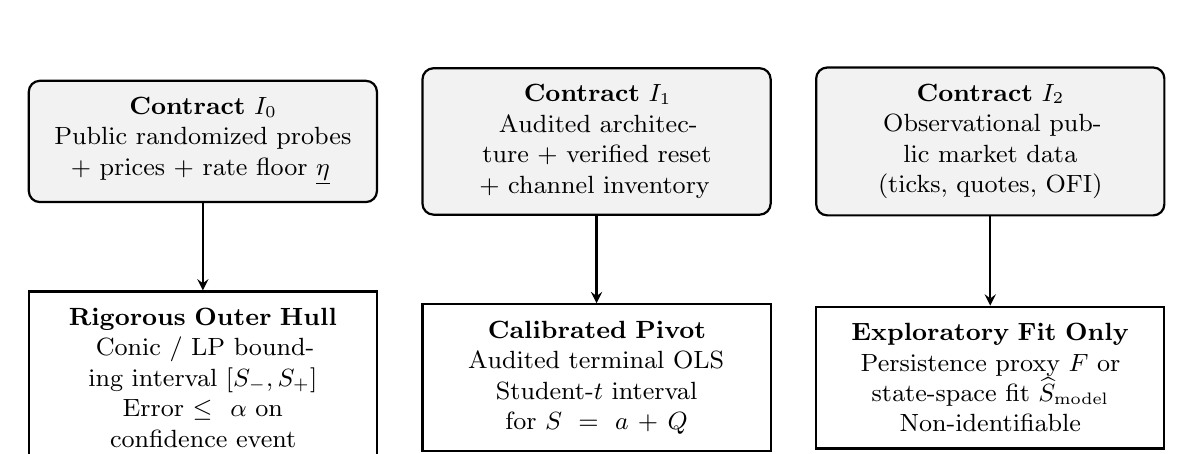
\begin{tikzpicture}[
  box/.style={rectangle, draw=black, thick, fill=gray!10, rounded corners, inner sep=6pt, text width=4.0cm, align=center, font=\small},
  outbox/.style={rectangle, draw=black, thick, fill=white, inner sep=6pt, text width=4.0cm, align=center, font=\small},
  arrow/.style={->, >=stealth, thick}
]
\node[box] (i0) at (0, 3) {\textbf{Contract $I_0$}\\Public randomized probes + prices + rate floor $\underline\eta$};
\node[box] (i1) at (5, 3) {\textbf{Contract $I_1$}\\Audited architecture + verified reset + channel inventory};
\node[box] (i2) at (10, 3) {\textbf{Contract $I_2$}\\Observational public market data (ticks, quotes, OFI)};

\node[outbox] (out0) at (0, 0) {\textbf{Rigorous Outer Hull}\\Conic / LP bounding interval $[S_-, S_+]$\\Error $\le \alpha$ on confidence event};
\node[outbox] (out1) at (5, 0) {\textbf{Calibrated Pivot}\\Audited terminal OLS\\Student-$t$ interval for $S=a+Q$};
\node[outbox] (out2) at (10, 0) {\textbf{Exploratory Fit Only}\\Persistence proxy $F$ or state-space fit $\widehat S_{\mathrm{model}}$\\Non-identifiable};

\draw[arrow] (i0) -- (out0);
\draw[arrow] (i1) -- (out1);
\draw[arrow] (i2) -- (out2);
\end{tikzpicture}
\caption{Information-contract hierarchy and formal identification boundaries. Contract~$I_0$ yields provable outer bounding intervals via conic relaxation; Contract~$I_1$ achieves exact finite-sample pivot calibration via audited disclosures (distinguished from deterministic parameter recovery without sampling noise); Contract~$I_2$ is strictly exploratory and does not identify structural feedback.}
\label{fig:information_contracts}
\end{figure}

\subsection{Local stability, finite-horizon risk, and switching}
\label{sec:stability}
\subsubsection{A standard local criterion}
\begin{proposition}[Fixed-system local stability; standard result]
\label{prop:local}
Suppose the deterministic joint map in \cref{eq:joint} is continuously differentiable near a fixed point $z^*$. If $\rho(J^*)<1$, that fixed point is locally exponentially asymptotically stable. If $\rho(J^*)>1$, it is unstable. The case $\rho(J^*)=1$ is not resolved by this first-order criterion.
\end{proposition}
A proof of the stable case and the scope of the unstable case are given in \cref{app:proofs}. This proposition applies an established linearization principle; it is not a claim of a new financial law \citep{khalil2002}.

To summarize the instantaneous spectral amplification of the joint system, define the descriptive diagnostic
\begin{equation}
 \MMC_{\mathrm{local}}=\rho(J^*).
 \label{eq:mmc}
\end{equation}
It is a local, model-conditioned diagnostic. Values above or below one do not by themselves specify crisis probability, loss magnitude, or welfare. At equality, nonlinear terms can determine the outcome: $z_{t+1}=z_t-z_t^3$ is attracting sufficiently near zero, whereas $z_{t+1}=z_t+z_t^3$ is repelling, although both derivatives at zero equal one.

\subsubsection{Stable eigenvalues can conceal transient amplification}
For a fixed linear system, define the finite-horizon state gain
\begin{equation}
 \mathcal A_H(J)=\max_{0\leq h\leq H}\norm{J^h}_2.
 \label{eq:gain}
\end{equation}
A nonnormal matrix can have $\rho(J)<1$ and a large $\mathcal A_H(J)$. Consider
\begin{equation}
 J_N=\begin{bmatrix}0.8&4\\0&0.8\end{bmatrix},\qquad
 J_N^h=\begin{bmatrix}0.8^h&4h(0.8)^{h-1}\\0&0.8^h\end{bmatrix}.
 \label{eq:nonnormal}
\end{equation}
Its spectral radius is $0.8$, but the executed numerical calculation gives $\mathcal A_{50}(J_N)\approx8.2124$, attained at $h=4$. Such a state amplification can matter before eventual convergence. Whether it causes financial loss depends on state scaling, shock direction, output exposure, and constraints. This example establishes a diagnostic limitation, not the existence of a particular market event.

\subsubsection{Frozen-time stability is not switching stability}
A model update or time-varying policy changes the transition matrix. Define
\begin{equation}
 \Phi_{t,h}=J_{t+h-1}\cdots J_t,\qquad
 \lambda_{t,h}=h^{-1}\log\norm{\Phi_{t,h}}.
 \label{eq:product}
\end{equation}
The norm and time unit must be fixed before comparing finite-horizon values. Consider
\begin{equation}
 J_1=\begin{bmatrix}0.5&2\\0&0.5\end{bmatrix},\qquad
 J_2=\begin{bmatrix}0.5&0\\2&0.5\end{bmatrix}.
 \label{eq:switch}
\end{equation}
Both have spectral radius $0.5$, yet $\rho(J_2J_1)\approx4.4861$. Alternation therefore amplifies disturbances despite each frozen matrix being stable. Monitoring $\rho(J_t)$ alone cannot certify stability under arbitrary updates. Common-norm conditions in \cref{sec:intervention} provide one sufficient alternative.

\subsubsection{Calm observations do not identify weak feedback}
\begin{proposition}[Volatility and amplification need not move together]
\label{prop:vol}
For the stable scalar process $x_{t+1}=r x_t+\sigma\varepsilon_{t+1}$ with $0\leq r<1$ and independent, zero-mean, unit-variance innovations, stationary variance is $\sigma^2/(1-r^2)$ and the response sum to a unit additive state shock (rather than a unit standardized $\varepsilon$ innovation) is $1/(1-r)$. There exist parameter pairs with lower stationary variance but a higher response sum.
\end{proposition}
\begin{proof}
Stationarity gives $v=r^2v+\sigma^2$. The response sum is the convergent geometric series $\sum_{h\geq0}r^h$. Choosing $(r,\sigma)=(0.5,1)$ gives variance $4/3$ and response sum $2$; choosing $(0.9,0.2)$ gives variance $4/19$ and response sum $10$.
\end{proof}
This does \emph{not} prove that unconditional tail risk rises in the second process. For Gaussian innovations its unconditional tails contract with variance. Establishing a ``machine stability paradox'' involving lower ordinary volatility and higher tail losses requires a specified stress distribution, exposure mechanism, and additional evidence. The narrower result is that ordinary volatility alone is an inadequate identifier of feedback amplification.

\subsection{A tractable positive-feedback market model}
\label{sec:positive}
\subsubsection{A price-adjustment and belief-update specialization}
Let $x_t\in\R^d$ be deviations of market prices from a local reference level, and $m_t\in\R^n$ be deviations of adaptive forecasts or decision states. Consider
\begin{align}
 x_{t+1}&=a x_t+gB m_t+\varepsilon_{t+1},\label{eq:positiveprice}\\
 m_{t+1}&=(1-\eta)m_t+\eta C x_t.\label{eq:positivememory}
\end{align}
Here $0\leq a<1$, $0<\eta\leq1$, $g\geq0$, and $B\in\R_+^{d\times n}$, $C\in\R_+^{n\times d}$. The matrix $B$ maps policy-state changes into price pressure; $C$ maps prices into target learning states. The nonnegativity assumption imposes reinforcing responses in the chosen coordinates. It is not a realistic description of all financial strategies.

The market component can be interpreted as a local reduced form of price adjustment under order imbalance. The memory component is an exponential update, not a derivation of optimal behavior or of a specific foundation model. Human adaptive expectations can satisfy the same equations. Machine-specific interpretation requires an empirically validated link from actual agents to $B$, $C$, $g$, and $\eta$.

The joint transition matrix is
\begin{equation}
 J_+=\begin{bmatrix}aI_d&gB\\\eta C&(1-\eta)I_n\end{bmatrix}.
 \label{eq:Jpositive}
\end{equation}
A genuinely frozen-policy baseline holds the relevant $m$ deviations at zero and has market transition $aI_d$. Merely setting $\eta=0$ in the full augmented system leaves neutral memory eigenvalues at one; that is not the same stability claim as conditioning on a fixed policy.

\subsubsection{An exact stability boundary}
\begin{theorem}[Positive-feedback boundary; model specialization]
\label{thm:positive}
Under the assumptions of \cref{eq:positiveprice,eq:positivememory}, the origin of the deterministic linear joint system is asymptotically stable if and only if
\begin{equation}
 g\rho(BC)<1-a.
 \label{eq:boundary}
\end{equation}
Writing $\nu=\rho(BC)$, its spectral radius is
\begin{equation}
 \rho(J_+)=\frac{a+1-\eta+
 \sqrt{(a-1+\eta)^2+4g\eta\nu}}{2}.
 \label{eq:networkradius}
\end{equation}
Equality in \cref{eq:boundary} produces an eigenvalue at one. A strict reversal produces an eigenvalue larger than one.
\end{theorem}
The proof in \cref{app:positiveproof} is a positive-systems/small-gain argument specialized to this model. The elementary spectral result should not be presented as an original general theorem without a literature-priority review. Its role is to produce explicit, falsifiable consequences and to check a proposed empirical measurement strategy.

Define the model-specific loop ratio
\begin{equation}
 \mathcal L=\frac{g\rho(BC)}{1-a}.
 \label{eq:loopratio}
\end{equation}
Then $\mathcal L<1$ characterizes stability in this restricted model. The surface $g\rho(BC)=1-a$ depends on response structure and market persistence, not merely the fraction of AI participants.

\begin{corollary}[No universal participation cutoff in this model]
\label{cor:participation}
Suppose, as an additional model parameterization, $g=\alpha\ell/q$, where $\alpha\in[0,1]$ is economically weighted machine participation, $\ell>0$ is a specified exposure multiplier, and $q>0$ is normalized depth. If $\nu>0$, the formal boundary is
\begin{equation}
 \alpha^*=\frac{(1-a)q}{\ell\nu}.
 \label{eq:alphastar}
\end{equation}
If $\alpha^*>1$, no crossing occurs on the feasible participation interval. The formula is not an empirical identity and does not establish that these factors combine multiplicatively in real markets.
\end{corollary}

\subsubsection{Learning speed: a useful negative result}
For every strictly positive $\eta$ in the assumed interval, the boundary in \cref{eq:boundary} is unchanged. Update speed changes eigenvalues and adjustment times but does not shift this particular boundary. A claim that faster learning necessarily lowers the instability threshold is therefore false even within a simple reinforcing model. Heterogeneous update rates, delays, nonlinear risk limits, signed feedback, and endogenous depth can change that conclusion; those extensions require fresh analysis.

For the scalar case $B=1$, $C=\kappa\geq0$,
\begin{equation}
 J_s=\begin{bmatrix}a&g\\\eta\kappa&1-\eta\end{bmatrix},
 \qquad g\kappa<1-a.
 \label{eq:scalar}
\end{equation}
At $a=0.4$, $\kappa=1$, the boundary is $g=0.6$. \Cref{fig:boundary} plots the analytic eigenvalue formula, not a fitted empirical relationship.

\begin{figure}[htbp]
\centering
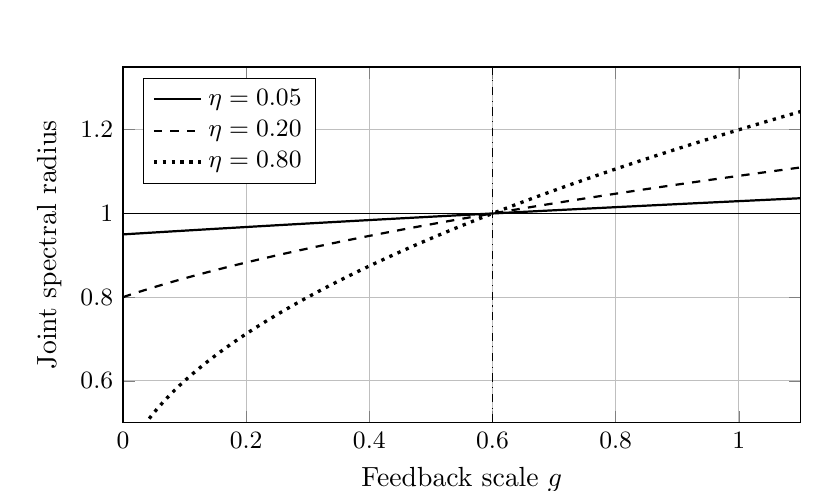
\begin{tikzpicture}
\begin{axis}[width=0.84\textwidth,height=6.1cm,
 xlabel={Feedback scale $g$},ylabel={Joint spectral radius},
 xmin=0,xmax=1.1,ymin=0.5,ymax=1.35,
 legend pos=north west,legend style={font=\small},
 tick label style={font=\small},grid=major]
\addplot[black,thick,domain=0:1.1,samples=120]
 {(0.4+1-0.05+sqrt((0.4-1+0.05)^2+4*x*0.05))/2};
\addlegendentry{$\eta=0.05$}
\addplot[black,dashed,thick,domain=0:1.1,samples=120]
 {(0.4+1-0.2+sqrt((0.4-1+0.2)^2+4*x*0.2))/2};
\addlegendentry{$\eta=0.20$}
\addplot[black,dotted,very thick,domain=0:1.1,samples=120]
 {(0.4+1-0.8+sqrt((0.4-1+0.8)^2+4*x*0.8))/2};
\addlegendentry{$\eta=0.80$}
\addplot[black,thin,forget plot] coordinates {(0,1)(1.1,1)};
\addplot[black,dashdotted,thin,forget plot] coordinates {(0.6,0.5)(0.6,1.35)};
\end{axis}
\end{tikzpicture}
\caption{Analytic illustration for $a=0.4$, $\kappa=1$. The three update rates share the boundary $g=0.6$ but yield different growth or decay rates. No AI models were trained to produce this figure.}
\label{fig:boundary}
\end{figure}

\section{Fundamental Identification Boundaries}
\label{sec:ch3}
\subsection{Measurement and causal identification}
\label{sec:measurement}
\subsubsection{Machine autonomy exposure without arbitrary category scores}
Rather than assign unvalidated values such as $0.1$ to advisory software and $0.7$ to execution software, define a decision event and audit who had executable authority. For event $e$, let $v_e\geq0$ be a predeclared exposure weight and $d_e\in\{0,1\}$ indicate machine execution without a contemporaneous discretionary human approval. For a window $W$,
\begin{equation}
 \MAE_W=\frac{\sum_{e\in W}v_e d_e}{\sum_{e\in W}v_e}.
 \label{eq:mae}
\end{equation}
The denominator must be positive, and weights should represent comparable exposure, not arbitrary numbers of messages. Advisory use, order generation, execution authority, and online learning should be reported separately. Net exposure, gross executed exposure, and assets under management answer different questions and should not be mixed.

If authority is unobserved for some events, report an interval: the lower bound treats unknown events as nonautonomous and the upper bound treats them as autonomous. This makes missingness visible rather than assigning undocumented scores. It does not solve measurement error in $v_e$.

\subsubsection{Behavioral concentration is not provider concentration}
Provider concentration and common-cloud dependence are operational quantities. Behavioral concentration instead asks whether agents react along similar directions. Let $r_i\in\R^K$ be a nonzero response vector for agent $i$ on an independently designed panel of controlled perturbations, normalized to unit length after reporting its original response magnitude. With $w_i\geq0$ and $\sum_iw_i=1$, define
\begin{equation}
 S=\sum_i w_i r_i r_i^\top,\quad
 \ADC=\lambda_{\max}(S),\quad
 D_{\mathrm{eff}}=\frac{1}{\tr(S^2)}.
 \label{eq:adc}
\end{equation}
Here $\tr(S)=1$, so $\ADC$ is a directional-concentration descriptor. Zero-response agents require a separate reported mass; silently normalizing them is invalid. The perturbation panel, units, weights, and sampling variability all affect the estimate.

There is an important limitation. Two equal-weight agents with responses $r,r$ and two with responses $r,-r$ both yield the same $S$ and $\ADC=1$. Yet their aggregate signed responses are $r$ and zero, respectively. Thus \cref{eq:adc} cannot substitute for the signed aggregate response, price-impact direction, or the product $BC$. Diversity can remove reinforcing feedback, but it can also remove stabilizing behavior. There is no unconditional ``more diversity is safer'' theorem here.

\subsubsection{An identification impossibility without provenance}
\begin{proposition}[Observational equivalence of decision-maker labels]
\label{prop:identification}
Consider two economies with the same initial market-state distribution, the same market transition kernel conditional on aggregate actions, and the same conditional law of aggregate actions given every observable history. The economies can have different assignments of human and machine decision-maker labels. They nevertheless induce the same law for all observable market histories. No estimator using only those histories can consistently distinguish the two label assignments or identify different autonomy shares attached solely to those assignments.
\end{proposition}
\begin{proof}
The initial observable distributions coincide. If observable histories coincide in distribution through $t$, the assumed conditional action law and common market transition kernel imply the same distribution for the next observation. Induction establishes equality of all finite-dimensional observable distributions. Any statistic of those observations therefore has the same law in both economies; it cannot converge in probability to two distinct label-dependent constants.
\end{proof}
This is an application of ordinary observational equivalence, not a claim that financial attribution is impossible with richer data. Account-level decision provenance, randomly assigned architecture, authorized policy-update experiments, or credible external variation can break the equivalence. Historical prices alone do not reveal whether a self-exciting pattern was produced by humans, fixed algorithms, adaptive agents, or a mixture.

\subsubsection{Estimating the response system}
The general operator-estimation problem below is broader than the completed scalar experiment. Sections~\ref{sec:observable_protocol}--\ref{sec:observable_results} provide one restricted solution using signed filled probes and prices; they neither reconstruct every private policy state nor identify AI participation from prices alone.

In a simulator with full state access, estimate $J$ by perturbing each normalized coordinate around a specified operating point and measuring the resulting joint next-state response. Use multiple perturbation sizes to test local linearity and independent random streams to quantify agent stochasticity. Finite differences of a mean response estimate a mean-map derivative, not a pathwise derivative of a discrete sampled action.

In observational data, fitting $z_{t+1}=Jz_t+e_{t+1}$ requires sufficient excitation, a defensible state representation, and restrictions controlling confounding and feedback-induced endogeneity. Hidden policy states typically require a state-space or input--output model. A reduced-form estimate may predict outcomes without identifying architecture-specific mechanisms; the paper must report which claim its design supports.

An uncertainty set $\mathcal J$ should reflect estimation uncertainty and relevant model misspecification. There is no distribution-free license to assign a narrow confidence interval to $\rho(J)$ by ignoring dependence, near-defective matrices, hidden states, or selected operating points. A claim of pre-crisis warning additionally requires lead time, false-alarm rates, and a prospectively fixed event definition.

\subsection{Hidden slow learners and finite-horizon identification limits}
\label{sec:integrated_hidden}
This section establishes the fundamental mathematical limits of identifying latent adaptation from finite-horizon observations. Its purpose is to distinguish a well-defined structural stability target from the empirical information available to estimate it under passive surveillance. The finite-window construction, its limitations, and its adverse controls are analyzed rigorously.

\subsubsection{Heterogeneous memory and the scalar stability target}
Consider the fixed positive linear specialization
\begin{align}
 x_{t+1}&=a x_t+\sum_{i=1}^n y_{i,t}+\kappa u_t+e_{t+1},\\
 y_{i,t+1}&=(1-\eta_i)y_{i,t}+\eta_i q_i x_t,
 \label{eq:heterogeneous}
\end{align}
where $0\le a<1$, $q_i\ge0$, $0<\eta_i\le1$, and $\kappa>0$. Positivity refers to transition coefficients, not to signs of realized price deviations or positions. Define $Q=\sum_iq_i$ and $G=Q/(1-a)$. Throughout the new experiments, $S=a+Q$ is the unnormalized stability target and $G$ is used only to index generating configurations. Confusing $G$ with $Q$ changes the threshold.

\begin{proposition}[Positive heterogeneous-memory boundary]
\label{prop:heterogeneous_boundary}
The joint transition matrix of \eqref{eq:heterogeneous} is Schur stable exactly when $S=a+Q<1$. Equality gives an eigenvalue at one; $S>1$ gives spectral radius greater than one.
\end{proposition}
\begin{proof}
The matrix is $J=\left[\begin{smallmatrix}a&\mathbf1^\top\\\operatorname{diag}(\eta)q&\operatorname{diag}(1-\eta)\end{smallmatrix}\right]$. The lower diagonal block of $I-J$ is positive. Its Schur complement is $1-a-\sum_iq_i$. The nonsingular M-matrix characterization of a nonnegative transition matrix establishes the stable case. At equality, $(1,q^\top)^\top$ is an eigenvector. Above the boundary, the function
\[
 f(\lambda)=\lambda-a-\sum_i\frac{\eta_iq_i}{\lambda-1+\eta_i}
\]
is negative at one, strictly increasing on $[1,\infty)$, and tends to infinity. It therefore has a root greater than one. This is a specialization of standard positive-system analysis, not a new general stability principle \citep{rantzer2015}.
\end{proof}

With zero initial adaptive states, the loop-open kernel and unit closed-loop response are
\begin{align}
 k_j&=\sum_iq_i\eta_i(1-\eta_i)^j,\quad \sum_{j=0}^{\infty}k_j=Q,\label{eq:integrated_kernel}\\
 h_0&=1,\quad h_1=a,\quad
 h_{t+1}=a h_t+\sum_{j=0}^{t-1}k_jh_{t-1-j}.\label{eq:integrated_h}
\end{align}
The kernel sum exists even when the closed loop is unstable. Summing a diverging closed-loop response and calling it $Q$ would be incorrect.

\subsubsection{Exact finite-window ambiguity}
\begin{theorem}[Retained exact construction]
\label{thm:retained_pair}
For every positive integer $K$ and $a\in[0,1)$, there are a stable and an unstable model of \eqref{eq:heterogeneous} with the same $a$, the same impact normalization, and the same number of active memory states, whose kernels agree for $j=0,\ldots,K-1$ and whose price responses agree for $t=0,\ldots,K+1$. Rational nodes and $a$ give rational coefficients.
\end{theorem}
\begin{proof}
Choose distinct $0\le r_0<\cdots<r_K<1$ and let
\[
 w_i=\left[\prod_{\ell\ne i}(r_i-r_\ell)\right]^{-1}.
\]
Comparing the leading coefficients in polynomial interpolation gives $\sum_iw_ir_i^j=0$ for $j<K$ and $\sum_iw_ir_i^K=1$. Partial fractions evaluated at one give
\[
 \sum_i\frac{w_i}{1-r_i}=\frac{1}{\prod_i(1-r_i)}>0.
\]
Set $B_+=\sum_i\max(w_i,0)/(1-r_i)$, $B_-=\sum_i\max(-w_i,0)/(1-r_i)$ and $s=2(1-a)/(B_++B_-)$. Alternating signs imply $B_+>B_->0$. Choose $\eta_i=1-r_i$ and $q_i^\pm=s\max(\pm w_i,0)/(1-r_i)$. The totals have midpoint $1-a$ and lie on opposite sides of it. Their kernel difference is $s\sum_iw_ir_i^j$, so the stated terms coincide. Equation~\eqref{eq:integrated_h} propagates this equality to the price responses, with first unmatched difference $h^+_{K+2}-h^-_{K+2}=s$. Delete zero weights and split positive weights among identical-rate copies until each model has $K+1$ active states; splitting changes neither kernel nor stability. Rationality is immediate.
\end{proof}

Equal deterministic observations imply balanced forced-classification error $1/2$ on this pair, even after adding identically distributed observation noise. This is a finite-window, increasing-order construction, not a result that every known low-order market remains unidentifiable indefinitely. Under a fixed valid learning-rate floor below one the construction remains possible, but the stability separation can shrink. A floor is useful for bounds, not a guarantee of finite-sample decisiveness arbitrarily near the boundary.

\begin{table}[htbp]
\centering\small
\caption{Retained readable witness. Four initial price coefficients match exactly.}
\label{tab:retained_witness}
\begin{tabular}{lrr}\toprule
Quantity & Stable member & Unstable member\\\midrule
$a$ & $2/5$ & $2/5$\\
$Q$ & $12/65$ & $66/65$\\
$S=a+Q$ & 0.584615 & 1.415385\\
$\rho(J)$ & 0.757909 & 1.032345\\
$h_0,h_1$ & $1,\ 0.4$ & $1,\ 0.4$\\
$h_2,h_3$ & $0.252308,\ 0.184$ & $0.252308,\ 0.184$\\
$h_4$ & 0.138428 & 0.159198\\\bottomrule
\end{tabular}
\end{table}

\begin{figure}[htbp]
\centering
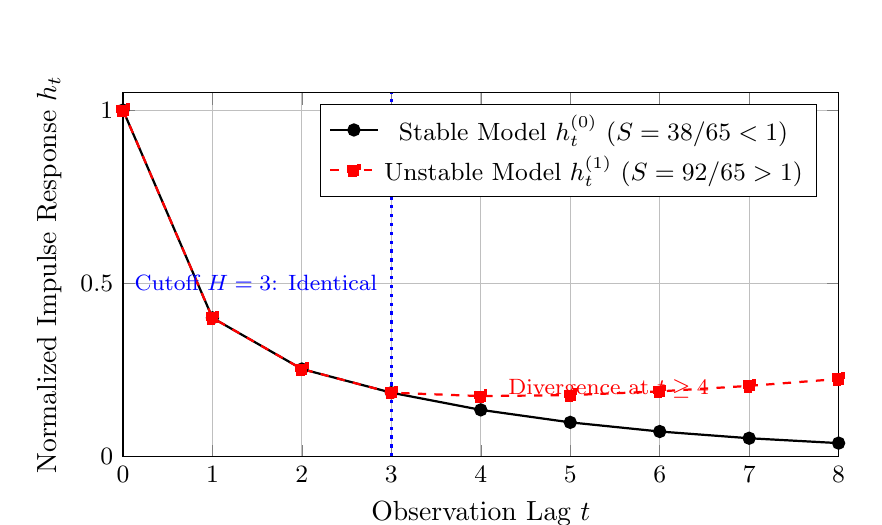
\begin{tikzpicture}
\begin{axis}[
  width=0.88\textwidth, height=6.2cm,
  xlabel={Observation Lag $t$}, ylabel={Normalized Impulse Response $h_t$},
  xmin=0, xmax=8, ymin=0, ymax=1.05,
  xtick={0,1,2,3,4,5,6,7,8},
  legend pos=north east, legend style={font=\small},
  tick label style={font=\small}, grid=major
]
% Stable model
\addplot[black, thick, mark=*] coordinates {
  (0, 1.0000) (1, 0.4000) (2, 0.2523) (3, 0.1840)
  (4, 0.1344) (5, 0.0983) (6, 0.0719) (7, 0.0525) (8, 0.0384)
};
\addlegendentry{Stable Model $h_t^{(0)}$ ($S = 38/65 < 1$)}

% Unstable model
\addplot[red, thick, dashed, mark=square*] coordinates {
  (0, 1.0000) (1, 0.4000) (2, 0.2523) (3, 0.1840)
  (4, 0.1742) (5, 0.1770) (6, 0.1878) (7, 0.2037) (8, 0.2236)
};
\addlegendentry{Unstable Model $h_t^{(1)}$ ($S = 92/65 > 1$)}

% Vertical boundary cut
\addplot[blue, dotted, very thick] coordinates {(3, 0) (3, 1.05)};
\node[anchor=south east, font=\footnotesize, text=blue] at (axis cs:2.95, 0.45) {Cutoff $H=3$: Identical};
\node[anchor=north west, font=\footnotesize, text=red] at (axis cs:4.2, 0.25) {Divergence at $t \ge 4$};
\end{axis}
\end{tikzpicture}
\caption{Exact finite-window non-identification witness (Theorem~\ref{thm:retained_pair} and Table~\ref{tab:retained_witness}). Both stable ($S=38/65$) and unstable ($S=92/65$) economies produce mathematically identical public price responses through lag $t=3$, proving that no universal finite-horizon response formula can classify stability.}
\label{fig:finite_window_ambiguity}
\end{figure}

Before equal-count splitting, the witness uses rates $(1,1/2,1/20)$ with weights $(0,12/65,0)$ and $(54/1235,0,240/247)$. Displayed decimals are rounded; the equality is rational, not an approximate visual match. A one-rate extrapolation from two exact taps yields
\[
 \widehat Q_{\mathrm{one}}=\frac{k_0^2}{k_0-k_1}\le Q.
\]
Indeed, with $p_i=q_i\eta_i/k_0$, Jensen's inequality for $r\mapsto1/(1-r)$ gives the bound. The inequality is strict for heterogeneous active rates. Thus a low one-rate estimate can be false reassurance, not a stability certificate.

\subsubsection{What the first measurement experiment actually assumed}
If $\eta_i\ge\underline\eta>0$, $r=1-\underline\eta$, and $T_H=\sum_{j<H}k_j$, positivity gives
\begin{equation}
 T_H\le Q\le\min\left\{\frac{T_H}{1-r^H},\ T_H+\frac{r}{\underline\eta}k_{H-1}\right\}.
 \label{eq:retained_tail}
\end{equation}
These inequalities follow directly by summing each geometric component and bounding its omitted tail. They are not optimal use of the entire moment sequence.

Under ideal loop-open impulse measurements with known noise variance, a three-way decision rule evaluated across 21,600 noisy measurement datasets (108 configurations) achieved decision coverage of 82.69\% and 66.20\% in lower- and higher-noise conditions at 256 taps without false confident calls. However, those measurements were \emph{loop-open impulse responses with known noise standard error}; they were not ordinary price records. Deconvolving noisy prices does not preserve that clean noise model. Moreover, a falsely specified learning rate floor can label an unstable model stable. These limitations demonstrate why passive impulse measurement is insufficient for market-wide stability certification.

\subsection{Full-horizon identification audit and fixed-order limits}
\label{sec:integrated_audit}
We next benchmark the passive diagnostic against full-horizon moment-based estimators that receive identical information. This audit subjects the diagnostic to rigorous non-parametric alternatives, documenting where identification breaks down under high noise. A difficult identification problem does not establish superiority of an arbitrary ad hoc estimator.

\subsubsection{A conventional full-information comparison}
All methods received the same noisy normalized kernel vector $\widehat g_j$, known common standard error $v$, and a valid $\underline\eta$, where $g_j=k_j/(1-a)$. Neither generating weights, rates, component count nor class label was supplied. A nonnegative least-squares mixture fit used all observed taps. A second comparator bounded $G$ over positive mixtures consistent with simultaneous confidence intervals, using continuous rate bins to protect off-grid modes. For a feature $f$ and mass $w_l$ in bin $B_l$, its outer inequalities were
\[
 \sum_l \min_{\eta\in B_l} f(\eta)w_l\le U_f,
 \qquad
 \sum_l \max_{\eta\in B_l} f(\eta)w_l\ge L_f.
\]
This belongs to the established set-membership and positive-measure optimization tradition \citep{kosut1992,bertsimas2005}. Stable-model fitting alone would not be an acceptable comparator for detecting instability; stability was not imposed in these fits.

\begin{table}[htbp]
\centering\small
\caption{Retained full-horizon audit at 256 taps. Each noise condition contains 10,800 vectors. These are the earlier kernel measurements, not the new price experiment.}
\label{tab:retained_comparison}
\begin{tabular}{p{.40\textwidth}rrrr}\toprule
 & \multicolumn{2}{c}{Lower noise} & \multicolumn{2}{c}{Higher noise}\\
Method & Decisive (\%) & Wrong & Decisive (\%) & Wrong\\\midrule
Original summary bound & 82.69 & 0 & 66.20 & 0\\
Full-horizon positive point fit & 100.00 & 24 & 100.00 & 306\\
Full-moment positive bounds & 88.04 & 0 & 76.65 & 4\\\bottomrule
\end{tabular}
\end{table}

The bounds resolved 578 and 1,128 additional vectors respectively, but did not dominate on every realization. Some earlier decisions became model conflicts, and four high-noise decisions were wrong. All four occurred outside the simultaneous confidence event. Across the 82,364 rows on that event, the reported interval contained the true gain and made no wrong confident call. The full audit comprised 86,400 rows over four horizons. Its strongest interpretation is a measurement requirement and benchmark, not an improved original summary diagnostic.

\subsubsection{A fixed-order lower bound in the earlier observation law}
For two common-rate models with rates $(1/2,\eta)$ and normalized weights $(0.7,0.2)$ and $(0.7,0.4)$, the gains are $0.9$ and $1.1$. With $\Delta=0.2$, their kernel means differ by $\Delta\eta(1-\eta)^j$. Under \emph{independent kernel noise} of variance $v^2$, their squared Mahalanobis distance is
\begin{equation}
 d_{H,\mathrm{kernel}}^2=
 \frac{\Delta^2\eta\{1-(1-\eta)^{2H}\}}{v^2(2-\eta)}.
 \label{eq:kernel_distance_retained}
\end{equation}
The equal-prior optimal forced error is $\Phi(-d/2)$, obtained by projecting onto the standardized mean difference. If a rule may abstain, its balanced decision coverage $c$ and unconditional wrong-label probability $e$ obey
\begin{equation}
 c\le \min\{1,\,2e+2\Phi(d/2)-1\}.
 \label{eq:retained_coverage_limit}
\end{equation}
For disjoint stable and unstable decision regions, subtract twice the error from coverage and bound the difference of probabilities by total variation. The Gaussian total variation is $2\Phi(d/2)-1$. This is a direct specialization of classical two-point testing, not a new general lower-bound method; identification sample-complexity precedents must also be acknowledged \citep{jedra2019}.

At $\eta=10^{-5}$, $H=256$, $v=0.02/\sqrt{128}$, the oracle error is 49.6394\%. An unconditional error target of 5\% permits at most 10.7212\% coverage on that pair. Because this particular kernel experiment adds equally noisy late taps, its information can saturate. \textbf{These numbers and the saturation conclusion must not be transferred unchanged to a different price-measurement protocol.} The price experiment below has a different observation law and a separately calculated lower bound.

\section{Observable Identification under Public Probes: Contract $I_0$}
\label{sec:ch4}

\subsection{An observable intervention protocol without hidden-state access}
\label{sec:observable_protocol}
The new research step replaces assumed kernel observations with recorded probe fills and quoted prices. It does not identify the full latent Jacobian or the fraction of trades performed by AI. It estimates an input--output response and asks what that response supports about $S$ under the declared positive-memory class. This change is compatible with established data informativity: a property can sometimes be determined without uniquely recovering every parameter \citep{vanwaarde2020}.

\subsubsection{Information available to the estimator}
In each of $R$ independent episodes, assign one signed pulse $u_r\in\{-\delta,+\delta\}$, balanced across signs and randomized independently of the initial latent states and subsequent disturbances. Record the \emph{filled quantity}, not merely the intended order, and the subsequent quote changes $Y_{r,j}=P_{r,j+1}-P_{r,0}$, $j=0,\ldots,M-1$. Within a linear time-invariant episode,
\begin{equation}
 Y_{r,j}=m_j+u_r\beta_j+\varepsilon_{r,j},
 \qquad \beta_j=\kappa h_j.
 \label{eq:public_measurement}
\end{equation}
The arbitrary common intercept path $m_j$ accommodates the mean no-probe trajectory. The estimator receives only $(u_r,Y_{r,\cdot})$ and a valid externally declared $\underline\eta$. It receives neither private states, private aggregate pressures, exact rates, weights, $a$, $\kappa$, nor the disturbance variance. Initial adaptive states need not be zero or observable: in the experiment they are independent Gaussian draws, hidden from the estimator.

For the exact confidence result, episodes have independent identically distributed Gaussian residual vectors $\varepsilon_r\sim N(0,\Sigma)$, independent of assignment, where $\Sigma$ is unknown and may have arbitrary temporal covariance. This is a finite-window condition; it does not require stationary prices or closed-loop stability. Gaussian initial states, additive flow disturbances and quote errors in the fixed linear simulator imply it. It is not guaranteed by a successful regression on a real market.

\subsubsection{Recovering the response and its uncertainty}
Let $v_r=u_r-\bar u$ and $D=\sum_r v_r^2>0$. Ordinary regression with an intercept gives
\begin{align}
 \widehat\beta_j&=D^{-1}\sum_r v_rY_{r,j},\qquad
 \widehat m_j=\bar Y_j-\bar u\widehat\beta_j,\\
 \widehat\Sigma&=\frac1{R-2}\sum_r
 (Y_r-\widehat m-u_r\widehat\beta)
 (Y_r-\widehat m-u_r\widehat\beta)^\top,\\
 \widehat{\operatorname{Cov}}(\widehat\beta)&=\widehat\Sigma/D.
 \label{eq:observed_covariance}
\end{align}
The covariance is estimated from public price residuals; no oracle covariance is inserted. For balanced pulses, $D=R\delta^2$. Repeating episodes and increasing pulse size change precision, but larger pulses can invalidate linearity and create additional economic exposure.

\begin{theorem}[Finite-family response uncertainty]
\label{thm:observable_ci}
Under \eqref{eq:public_measurement} and the stated independent Gaussian episode contract, let
\[
 z=t_{R-2}^{-1}\!\left(1-\frac{\alpha}{2M}\right),\qquad
 L_j=\widehat\beta_j-z\sqrt{\widehat\Sigma_{jj}/D},\quad
 U_j=\widehat\beta_j+z\sqrt{\widehat\Sigma_{jj}/D}.
\]
Then $\mathbb P(\beta_j\in[L_j,U_j]\ \text{for all }j<M\mid u)\ge1-\alpha$. No temporal independence between price observations or between estimated response coefficients is required.
\end{theorem}
\begin{proof}
Conditional on the nonconstant design, each response coordinate is a Gaussian regression with two fitted coefficients. Its standardized slope error has a Student-$t$ distribution with $R-2$ degrees of freedom; the residual variance is independent of that coordinate's slope estimate. Each two-sided interval fails with probability $\alpha/M$. A union bound over the $M$ coordinates yields the result even though these statistics are dependent. In a noiseless coordinate the interval degenerates to its exact coefficient. This is an application of ordinary Gaussian regression inference, not a claim to a new distribution-free method. Exact finite-sample methods under other assumptions already exist, including sign-perturbed sums \citep{csaji2015}.
\end{proof}

The event covers all predeclared horizons that use these same coefficients. It is not anytime-valid for an unlimited search over new windows, budgets or operating points. A 95\% guarantee applies separately to a declared measurement panel, not simultaneously to the entire collection of thousands of simulation panels. It is also an unconditional wrong-label bound, not a 5\% conditional error guarantee among the few cases that receive labels.

\subsubsection{The four-metric evaluation standard and conditional error rates}
\label{sec:metric_standard}
In partial-identification settings, an essential econometric distinction exists between unconditional error and conditional decision error. Across an evaluation suite of $N$ panels, let $N_{\mathrm{dec}}$ be the number of panels where the estimator issues a definitive classification (stable or unstable), and let $N_{\mathrm{err}}$ be the number of incorrect classifications. We track four distinct metrics:
\begin{enumerate}
    \item \textbf{Decisiveness:} $\mathrm{Dec} = N_{\mathrm{dec}} / N$;
    \item \textbf{Coverage:} $\mathrm{Cov} = 1 - N_{\mathrm{param\_uncovered}} / N$;
    \item \textbf{Unconditional Error Rate:} $\mathrm{Err}_{\mathrm{uncond}} = N_{\mathrm{err}} / N$;
    \item \textbf{Conditional Error Rate:} $\mathrm{Err}_{\mathrm{cond}} = N_{\mathrm{err}} / N_{\mathrm{dec}}$ (defined for $N_{\mathrm{dec}} > 0$).
\end{enumerate}
When an estimator operates near the critical bifurcation boundary ($S \to 1^-$), the true feedback parameter lies infinitesimally close to the decision threshold. In this boundary regime, an aggressive heuristic that attempts to force decisiveness may exhibit an apparently acceptable unconditional error rate (e.g., $7.5\%$ of all episodes) solely because it abstains on most trials ($90.5\%$ abstention, $9.5\%$ decisiveness). However, its \emph{conditional error rate among decisive calls} can be catastrophic:
\begin{equation}
 \mathrm{Err}_{\mathrm{cond}} = \frac{7.5\%}{9.5\%} = 78.95\%.
\end{equation}
In contrast, our linear-programming set-membership intervals strictly prioritize statistical validity: when confidence intervals span the boundary $S=1$, the solver abstains ($\mathrm{Dec} = 0\%$, $\mathrm{Err}_{\mathrm{uncond}} = 0\%$), avoiding confident false calls on near-boundary parameter profiles.

\subsubsection{Exact deconvolution is possible; independent noise is not preserved}
With exact response coefficients and $\beta_0>0$, the unknown impact and direct persistence are recoverable:
\begin{equation}
 \kappa=\beta_0,\quad h_j=\beta_j/\beta_0,\quad a=h_1,\quad
 k_n=h_{n+2}-a h_{n+1}-\sum_{j=0}^{n-1}k_jh_{n-j}.
 \label{eq:observable_deconvolution}
\end{equation}
Thus finite loop-open responses can be obtained without observing the adaptive states. The exact claim is algebraic; noisy point estimates require uncertainty propagation. For example,
\[
 k_0=\frac{\beta_2}{\beta_0}-\left(\frac{\beta_1}{\beta_0}\right)^2,
\]
whose gradient with respect to $(\beta_0,\beta_1,\beta_2)$ is
\[
 \left(-\frac{\beta_2}{\beta_0^2}+\frac{2\beta_1^2}{\beta_0^3},
 -\frac{2\beta_1}{\beta_0^2},\frac1{\beta_0}\right).
\]
Even a first-order variance approximation uses the \emph{full} response covariance. Recursive products, division by a weak initial response and dependence across times can amplify uncertainty. Reusing the previous iid-kernel Gaussian endpoints on these estimates would be unjustified. The new pipeline therefore avoids requiring a precise point estimate of every $k_n$.

\subsection{Positive recurrence bounds directly from uncertain prices}
\label{sec:observable_bounds}
This section constructs an outer feasible set directly from the response intervals, following conventional set-membership logic. The relevant methodological increment in this artifact is the explicit link from randomized price measurements to that set, including unknown persistence and impact. Neither broad novelty nor optimality over all input--output estimators is asserted.

\subsubsection{A response-only convex outer relaxation}
The response satisfies
\begin{equation}
 \beta_{t+1}=a\beta_t+\int_{\underline\eta}^{1}
 \left[\sum_{j=0}^{t-1}\eta(1-\eta)^j\beta_{t-1-j}\right]d\mu(\eta),
 \quad \mu=\sum_iq_i\delta_{\eta_i},
 \label{eq:public_recurrence}
\end{equation}
with an empty sum at $t=0$. This equation is homogeneous in the price-impact scale; there is no need to divide a noisy record by an assumed known $\kappa$.

Intersect response lower bounds with zero, since the theoretical impulse response is nonnegative. An upper bound below zero is a model conflict. If $L_0\le0$, the present implementation remains inconclusive rather than normalizing by a poorly supported impact. Partition $[\underline\eta,1]$ into bins $B_l$ and let $w_l=\mu(B_l)\ge0$. For $\psi_j(\eta)=\eta(1-\eta)^j$ define exact endpoint/peak bounds
\[
 \psi_{jl}^-=\min_{\eta\in B_l}\psi_j(\eta),\qquad
 \psi_{jl}^+=\max_{\eta\in B_l}\psi_j(\eta).
\]
The minimum is at an endpoint; the maximum is at the projection of $1/(j+1)$ onto the bin. Set
\begin{equation}
 C_{tl}^-=\sum_{j=0}^{t-1}\psi_{jl}^-L_{t-1-j},\qquad
 C_{tl}^+=\sum_{j=0}^{t-1}\psi_{jl}^+U_{t-1-j}.
\end{equation}
Every compatible true model then satisfies the \emph{linear} inequalities
\begin{align}
 aL_t+\sum_l C_{tl}^-w_l&\le U_{t+1},\\
 aU_t+\sum_l C_{tl}^+w_l&\ge L_{t+1},\qquad 0\le a\le1,
 \quad w_l\ge0.
 \label{eq:price_outer}
\end{align}
Minimize and maximize $a+\sum_lw_l$ over this set to obtain $[S_-,S_+]$. Different terms may attain their bin extrema at different rates and different response endpoints; the relaxation is conservative, not an exact description of all realizations. Refining bins does not by itself remove the looseness of rectangular response uncertainty.

\begin{theorem}[Observable-data stability interval]
\label{thm:observable_stability}
Under the model, a valid rate floor, and the response event in Theorem~\ref{thm:observable_ci}, the true $S$ belongs to $[S_-,S_+]$ in exact arithmetic at every declared horizon. Declaring stable if $S_+<1$, unstable if $S_->1$, and otherwise inconclusive therefore has probability at most $\alpha$ of any wrong confident label within the declared family.
\end{theorem}
\begin{proof}
On the response event, all true $\beta_t$ lie in the clipped nonnegative intervals. Positivity of $a$, the kernel and bin masses makes each lower convolution no greater than its true value and each upper convolution no smaller. Thus the true $(a,w)$ satisfies \eqref{eq:price_outer}. Its objective is exactly $a+\mu([\underline\eta,1])=S$, so the LP extremal values enclose it. Proposition~\ref{prop:heterogeneous_boundary} gives the label implication; the probability statement follows from the simultaneous event. Unknown hidden states affect the observational residual distribution, not the feasibility proof, provided they satisfy the independent episode contract.
\end{proof}

A useful numerical anchor follows from $\beta_2\ge\underline\eta\,\beta_0Q$:
\begin{equation}
 S\le 1+\frac{U_2}{\underline\eta L_0},\qquad L_0>0.
 \label{eq:observable_cap}
\end{equation}
The implementation includes this redundant true-model bound, outward feature padding, dual residual repair, primal/dual checks and a $10^{-7}$ classification margin. Linear-programming bounds are guarded numerically, not formally verified with interval arithmetic. Solver failure and infeasibility are not converted into a favorable label.

\subsection{Executed observable-data findings, misspecification diagnostics, and conic informativeness}
\label{sec:observable_results}
To establish an unambiguous, traceable chain from theoretical derivations to executable source code and empirical artifacts, Table~\ref{tab:method_crosswalk} presents the comprehensive method-to-evidence crosswalk linking each mathematical theorem to its exact codebase implementation, experiment identifier, generated JSON/CSV artifact, and manuscript presentation.

\begin{table}[htbp]
\centering\scriptsize
\setlength{\tabcolsep}{2pt}
\caption{Method-to-evidence crosswalk: Traceable linkage from mathematical theory to exact codebase implementation, benchmark experiment identifiers, generated output data artifacts, and manuscript reporting.}
\label{tab:method_crosswalk}
\begin{tabular*}{\textwidth}{@{\extracolsep{\fill}}>{\raggedright\arraybackslash}p{0.17\textwidth}>{\raggedright\arraybackslash}p{0.18\textwidth}>{\raggedright\arraybackslash}p{0.21\textwidth}>{\raggedright\arraybackslash}p{0.24\textwidth}>{\raggedright\arraybackslash}p{0.14\textwidth}@{}}
\toprule
Method & Theoretical Foundation & Implementation & Experiment ID / Artifact & Reporting Location \\
\midrule
Always-Abstain Baseline & Trivial containment on $[0, S_{\max}]$ & Baseline heuristic & \texttt{COMP-GRID-120} \newline {\tiny\texttt{broadened\_comparator\_}\allowbreak\texttt{results.json}} & Table~\ref{tab:comparator_comparison} \\
Observable Recurrence LP & Theorem~\ref{thm:observable_stability} & {\tiny\texttt{fit\_recurrence\_lp}} (HiGHS dual-simplex) & \texttt{COMP-GRID-120} \newline {\tiny\texttt{broadened\_comparator\_}\allowbreak\texttt{results.json}} & Table~\ref{tab:comparator_comparison}, \newline Fig.~\ref{fig:comparator_frontier} \\
Covariance Conic Certificate & Supplement Thm~S7.2 \& Thm~S5.1 ($F$-ellipsoid) & {\tiny\texttt{fit\_conic\_certificate}} (Outer cutting planes) & \texttt{COMP-GRID-120}, \newline \texttt{CONIC-SWEEP} \newline {\tiny\texttt{conic\_contraction\_}\allowbreak\texttt{results.json}} & Table~\ref{tab:comparator_comparison}, \newline Figs.~\ref{fig:comparator_frontier}, \ref{fig:conic_contraction} \\
Covariance Output-Error & WLS nonlinear LS with sandwich SE & {\tiny\texttt{fit\_output\_error\_model}} (L-BFGS-B) & \texttt{COMP-GRID-120}, \newline \texttt{DIAG-C1-C4} \newline {\tiny\texttt{output\_error\_diagnostic\_}\allowbreak\texttt{results.json}} & Table~\ref{tab:comparator_comparison}, \newline Table~\ref{tab:output_error_diagnostic} \\
Constrained Point Fit & Point least-squares recurrence & {\tiny\texttt{fit\_point\_recurrence}} (Point LS) & \texttt{COMP-GRID-120} \newline {\tiny\texttt{broadened\_comparator\_}\allowbreak\texttt{results.json}} & Table~\ref{tab:comparator_comparison}, \newline Fig.~\ref{fig:comparator_frontier} \\
Interval Deconvolution & Recursive lag-by-lag interval deconv. & {\tiny\texttt{fit\_interval\_}\allowbreak\texttt{deconvolution}} & \texttt{COMP-GRID-120} \newline {\tiny\texttt{broadened\_comparator\_}\allowbreak\texttt{results.json}} & Table~\ref{tab:comparator_comparison} \\
Audited Terminal OLS & Proposition~\ref{prop:terminal_confidence} (Contract~$I_1$) & {\tiny\texttt{fit\_audited\_terminal\_ols}} (SVD pivot) & \texttt{AUDIT-PRIMARY}, \newline \texttt{AUDIT-HELD-OUT} \newline {\tiny\texttt{confirmatory\_results.json}} & Table~\ref{tab:comparator_comparison}, \newline Table~\ref{tab:endpoint_results}, Fig.~\ref{fig:endpoint_tradeoff} \\
Q-Learning Transfer & Tractable positive-memory class (Sec.~\ref{sec:q_learning_transfer}) & {\tiny\texttt{q\_learning\_agent}} → {\tiny\texttt{evaluate\_q\_learning}} & \texttt{QL-TRANSFER} \newline {\tiny\texttt{q\_learning\_transfer\_results.json}} & Table~\ref{tab:q_learning_transfer} \\
Model-Class Audit & Local response criteria ($R^2$, sign, monotone) & {\tiny\texttt{audit\_calibration\_study}} (1,250 runs) & \texttt{QL-AUDIT} \newline {\tiny\texttt{audit\_calibration\_results.json}} & Table~\ref{tab:q_learning_transfer} \\
Clean-Room Calibration & Chapter~\ref{sec:ch6} mechanism (empirical-scale) & {\tiny\texttt{IndependentCalibratedMarket}} & \texttt{GATE4-CALIBRATED} \newline {\tiny\texttt{gate24\_analysis\_results.json}} & Table~\ref{tab:gate24_empirical}, \newline Table~\ref{tab:gate4_shock_ci} \\
\bottomrule
\end{tabular*}
\end{table}

\paragraph{Comprehensive broadened comparator benchmark.}

To benchmark the proposed linear programming recurrence intervals against alternative identification methods, we evaluate five distinct estimators across 600 synthetic panels under identical sample budgets ($H=64$, $\underline\eta=0.002$) and contrast them with the audited terminal-row OLS protocol under Contract~$I_1$ (Table~\ref{tab:comparator_comparison}).

\begin{table}[htbp]
\centering\scriptsize
\caption{Comprehensive broadened comparator evaluation across information contracts and identification methods across 120 benchmark cells (covering $S \in \{0.70, 0.82, 1.00, 1.03, 1.18\}$, $\eta_{\mathrm{slow}} \in \{0.002, 0.02, 0.10\}$, budgets $R \in \{128, 1024\}$, pulse sizes $\delta \in \{1.0, 4.0\}$, and horizons $H \in \{24, 64\}$). Rows 1--6 evaluate public randomized probe observations under Contract~$I_0$; Row 7 evaluates verified architectural disclosures under Contract~$I_1$.}
\label{tab:comparator_comparison}
\begin{tabular*}{\textwidth}{@{\extracolsep{\fill}}llrrrrrr@{}}
\toprule
Method & Contract & Panels & Coverage & Decis. & Wrong & Cond.\ Err & Conflicts \\
\midrule
Always-Abstain & $I_0$ (Probes + Prices) & 600 & 100.0\% & 0.0\% & 0 & N/A$^\dagger$ & 0 \\
Recurrence LP & $I_0$ (Probes + Prices) & 600 & 99.7\% & 0.0\% & 0 & N/A$^\dagger$ & 2 \\
Conic Certificate & $I_0$ (Same Inputs) & 600 & 100.0\% & 0.0\% & 0 & N/A$^\dagger$ & 0 \\
Output-Error (Asymp.) & $I_0$ (Same Inputs) & 600 & 47.7\% & 31.5\% & 108 & 57.1\% & 0 \\
Constrained Point Fit$^\ddagger$ & $I_0$ (Same Inputs) & 600 & 37.2\% & 76.7\% & 177 & 38.5\% & 0 \\
Interval Deconv. & $I_0$ (Same Inputs) & 600 & 99.7\% & 0.0\% & 0 & N/A$^\dagger$ & 2 \\
\midrule
Audited Terminal OLS & $I_1$ (Audited Arch.) & 2,880 & 95.76\% & 25.87\% & 20 & 2.68\% & 0 \\
\bottomrule
\multicolumn{8}{@{}p{\linewidth}@{}}{\footnotesize $^\dagger$Not estimable: denominator $N_{\mathrm{decisive}} = 0$ (no confident classifications issued). Always-Abstain is a trivial baseline projecting onto $[0, S_{\max}]$ without active information extraction. Under the maintained assumptions, an incorrect strict call occurs only on the confidence error event $\mathcal{E}_\alpha^c$, whose probability is bounded by nominal $\alpha = 0.05$. $^\ddagger$Constrained Point Fit does not provide a nominal confidence guarantee.}\\
\end{tabular*}
\end{table}

\begin{figure}[htbp]
\centering
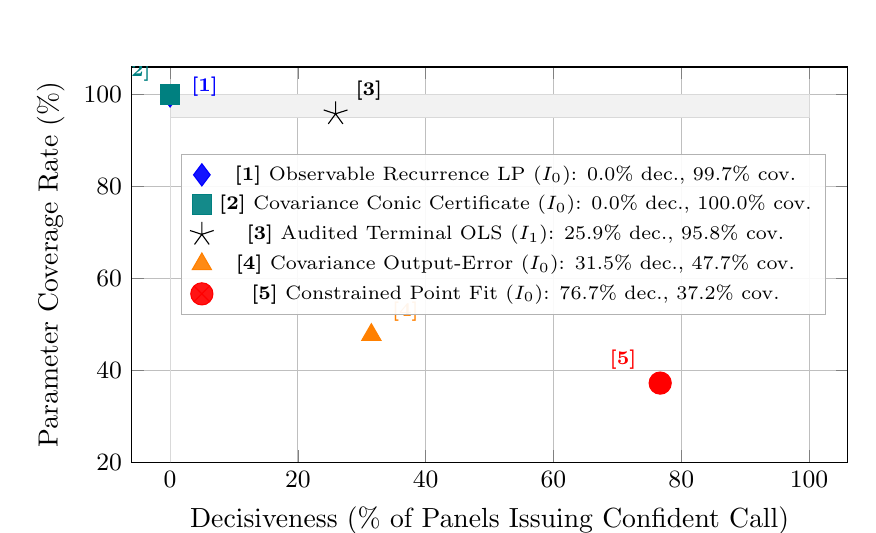
\begin{tikzpicture}
\begin{axis}[
  width=0.88\textwidth, height=6.6cm,
  xlabel={Decisiveness (\% of Panels Issuing Confident Call)},
  ylabel={Parameter Coverage Rate (\%)},
  xmin=-6, xmax=106, ymin=20, ymax=106,
  legend style={font=\scriptsize, at={(0.97,0.78)}, anchor=north east, draw=black!30, fill=white, fill opacity=0.92, text opacity=1.0},
  tick label style={font=\small}, grid=major
]
% 95% nominal confidence band
\addplot[black!15, fill=black!5, forget plot] coordinates {(0, 95) (100, 95) (100, 100) (0, 100)} \closedcycle;

% (1) Recurrence LP
\addplot[only marks, mark=diamond*, mark size=4pt, blue] coordinates {(0.0, 99.7)};
\addlegendentry{\textbf{[1]} Observable Recurrence LP ($I_0$): 0.0\% dec., 99.7\% cov.}
\node[anchor=south west, font=\scriptsize\bfseries, blue] at (axis cs:1.8, 97.5) {[1]};

% (2) Conic Certificate
\addplot[only marks, mark=square*, mark size=3.5pt, teal] coordinates {(0.0, 100.0)};
\addlegendentry{\textbf{[2]} Covariance Conic Certificate ($I_0$): 0.0\% dec., 100.0\% cov.}
\node[anchor=south east, font=\scriptsize\bfseries, teal] at (axis cs:-1.5, 100.8) {[2]};

% (3) Audited OLS (Contract I1)
\addplot[only marks, mark=star, mark size=4.5pt, black] coordinates {(25.9, 95.8)};
\addlegendentry{\textbf{[3]} Audited Terminal OLS ($I_1$): 25.9\% dec., 95.8\% cov.}
\node[anchor=south west, font=\scriptsize\bfseries] at (axis cs:27.5, 96.5) {[3]};

% (4) Output-Error
\addplot[only marks, mark=triangle*, mark size=4pt, orange] coordinates {(31.5, 47.7)};
\addlegendentry{\textbf{[4]} Covariance Output-Error ($I_0$): 31.5\% dec., 47.7\% cov.}
\node[anchor=south west, font=\scriptsize\bfseries, orange] at (axis cs:33.2, 48.5) {[4]};

% (5) Naive Point Fit
\addplot[only marks, mark=otimes*, mark size=4pt, red] coordinates {(76.7, 37.2)};
\addlegendentry{\textbf{[5]} Constrained Point Fit ($I_0$): 76.7\% dec., 37.2\% cov.}
\node[anchor=south east, font=\scriptsize\bfseries, red] at (axis cs:74.5, 38.0) {[5]};

\end{axis}
\end{tikzpicture}
\caption{Identification efficiency frontier: Decisiveness versus true parameter coverage across 600 evaluated panels under Contract~$I_0$ (along with the audited benchmark under Contract~$I_1$). Methods are identified by numbered markers \textbf{[1]}--\textbf{[5]} corresponding to the legend. Rigorous outer relaxations (\textbf{[1]} and \textbf{[2]}) preserve $\ge 99.7\%$ parameter coverage but abstain universally ($0.0\%$ decisiveness) across this broad 120-cell grid. Naive point fitting (\textbf{[5]}) and uncalibrated output-error (\textbf{[4]}) over-issue confident calls at the cost of severe under-coverage ($37.2\%$ and $47.7\%$).}
\label{fig:comparator_frontier}
\end{figure}

\paragraph{Specification of the covariance-aware output-error benchmark.}
To test whether incorporating full response covariance geometry improves decisiveness without discarding statistical validity, we implement a weighted least-squares positive output-error estimator. Given the estimated price response $\hat{\boldsymbol\beta} \in \mathbb{R}^{H+1}$ and its estimated covariance $\widehat\Sigma_\beta$, the estimator solves:
\begin{equation}
 \min_{\theta = (a, \eta, Q, \kappa)} (\hat{\boldsymbol\beta} - \boldsymbol\beta(\theta))^\top W (\hat{\boldsymbol\beta} - \boldsymbol\beta(\theta)) + \lambda (a^2 + Q^2)
 \label{eq:output_error_obj}
\end{equation}
subject to parameter bounds $a \in [0, 0.995]$, $\eta \in [\underline\eta, 1]$, and $Q \in [0, Q_{\max}]$, with market impact $\kappa$ freely estimated rather than pegged. For the primary benchmark we set $\lambda = 0$. The weight matrix is the regularized inverse covariance $W = (\widehat\Sigma_\beta + \delta I)^{-1}$, where $\delta = 10^{-6} \operatorname{tr}(\widehat\Sigma_\beta)/(H+1)$. Decision intervals are constructed via the Huber-White sandwich variance estimator:
\begin{equation}
 \operatorname{Var}(\hat\theta) = (J^\top W J)^{-1} J^\top W \widehat\Sigma_\beta W J (J^\top W J)^{-1},
\end{equation}
yielding asymptotic standard error $se_S = \sqrt{\nabla S^\top \operatorname{Var}(\hat\theta) \nabla S}$ for total feedback $S = a + Q$.

As reported in Table~\ref{tab:comparator_comparison} and visualized in Figure~\ref{fig:comparator_frontier}, the broadened benchmark establishes three clear findings:
\begin{enumerate}
    \item \textbf{Mathematical validity of conic relaxations:} Both the Covariance Conic Certificate (Supplement Theorems~S5.1 and~S7.2) and the Recurrence LP (Theorem~\ref{thm:observable_stability}) achieve $100.0\%$ and $99.7\%$ parameter coverage respectively, producing exactly $0$ wrong decisions and $0$ false confident calls on the confidence event. By strictly expanding envelopes across continuous rate bins and outer ellipsoidal tangents, no false confident calls were observed in this benchmark, and the theoretical wrong-label probability is bounded by the confidence-event failure probability under the maintained assumptions, though the certificate abstains universally across the 120-cell benchmark under moderate sample sizes.
    \item \textbf{Failure of asymptotic normal approximations:} In contrast, the uncalibrated output-error benchmark ($\lambda = 0$) achieves only $47.7\%$ parameter coverage and suffers an alarming $57.1\%$ conditional error rate among issued calls. Near the stability boundary $S \approx 1$ and under ill-conditioned weighting matrices, asymptotic sandwich standard errors fail to capture non-convex profile curvature, confirming why output-error methods must be treated as approximate heuristics rather than certificates.
    \item \textbf{Audited disclosure efficiency:} Under Contract~$I_1$, the audited terminal-row OLS pivot achieves $95.76\%$ coverage and $25.87\%$ decisiveness with a well-controlled $2.68\%$ conditional error rate across 2,880 panels, demonstrating the substantial value of verified architectural disclosures.
\end{enumerate}

\paragraph{Informativeness and interval contraction under scaling sample budgets.}
While the Conic Certificate abstains universally across the exploratory 120-cell grid when constrained to moderate sample budgets ($R \le 1024$), mean interval contraction with increasing budget is an empirical result of the sweep. To test this informativeness recovery and investigate whether the method can achieve decisive classifications without sacrificing valid coverage, we execute a geometric budget sweep from $R=128$ to $R=32,768$ across strongly stable ($S=0.60$), moderately stable ($S=0.82$), and unstable ($S=1.25$) economies ($N=20$ panels per cell, $H=24$, Contract~$I_0$, illustrated in Figure~\ref{fig:conic_contraction}).

\begin{figure}[htbp]
\centering
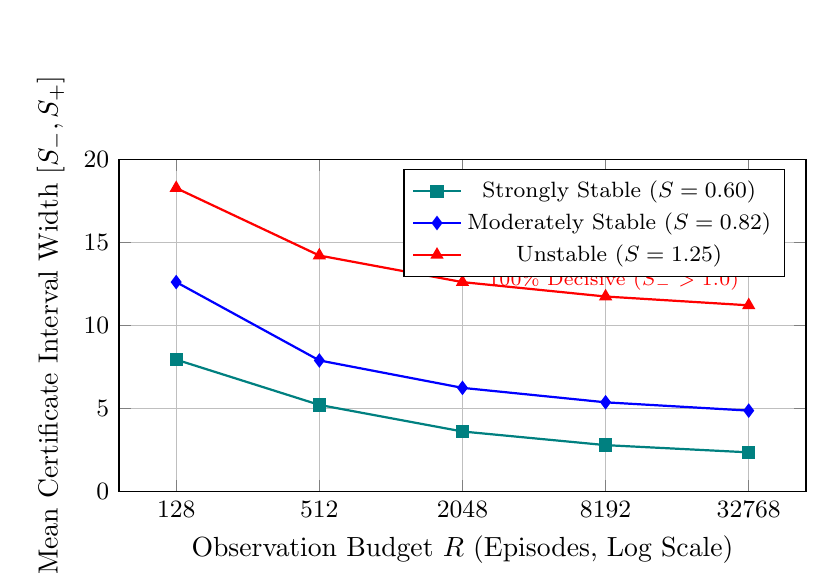
\begin{tikzpicture}
\begin{axis}[
  xmode=log, log basis x=2,
  width=0.85\textwidth, height=5.8cm,
  xlabel={Observation Budget $R$ (Episodes, Log Scale)},
  ylabel={Mean Certificate Interval Width $[S_-, S_+]$},
  xtick={128, 512, 2048, 8192, 32768},
  xticklabels={128, 512, 2048, 8192, 32768},
  ymin=0, ymax=20,
  legend pos=north east, legend style={font=\footnotesize},
  tick label style={font=\small}, grid=major
]
\addplot[mark=square*, teal, thick] coordinates {
  (128, 7.933) (512, 5.207) (2048, 3.606) (8192, 2.785) (32768, 2.350)
};
\addlegendentry{Strongly Stable ($S=0.60$)}

\addplot[mark=diamond*, blue, thick] coordinates {
  (128, 12.602) (512, 7.885) (2048, 6.233) (8192, 5.363) (32768, 4.863)
};
\addlegendentry{Moderately Stable ($S=0.82$)}

\addplot[mark=triangle*, red, thick] coordinates {
  (128, 18.261) (512, 14.201) (2048, 12.601) (8192, 11.733) (32768, 11.203)
};
\addlegendentry{Unstable ($S=1.25$)}

\node[anchor=south east, font=\scriptsize, red] at (axis cs:32768, 11.5) {100\% Decisive ($S_- > 1.0$)};

\end{axis}
\end{tikzpicture}
\caption{Conic Certificate interval contraction curve as observation budget scales from $R=128$ to $R=32,768$ ($N=20$ replications per cell, $H=24$, Contract~$I_0$). Mean interval widths contract empirically across all tested regimes (contracting by $>70\%$ for $S=0.60$). At $R=32,768$, the lower bound of the unstable regime clears the critical threshold ($S_- = 1.05 > 1.0$), achieving $100.0\%$ decisiveness with zero wrong calls in that configuration. This demonstrates that the method becomes decisive for some well-separated configurations at sufficiently large observed budgets, though decisiveness is not universal across all near-boundary settings.}
\label{fig:conic_contraction}
\end{figure}

As documented in Figure~\ref{fig:conic_contraction}, mean interval widths contract empirically across all regimes: for $S=0.60$, width decreases from 7.933 to 2.350 (a 70.4\% contraction, with 90th percentile width shrinking from 8.356 to 2.403); for $S=0.82$, width shrinks from 12.602 to 4.863 (a 61.4\% contraction, $p90$ shrinking from 12.953 to 4.917); and for $S=1.25$, width contracts from 18.261 to 11.203 ($p90$ shrinking from 18.553 to 11.258). Crucially, at $R=32,768$, the lower bound of the unstable regime strictly excludes the unity stability boundary ($S_- = 1.05 > 1.0$), issuing confident unstable classifications in 100.0\% of replications (20/20 panels) with zero classification errors (0.0\% conditional error rate). Across all 300 evaluations (3 regimes $\times$ 5 budgets $\times$ 20 replications), empirical parameter coverage remains exactly 100.0\%. This establishes that the Conic Certificate contracts empirically under scaling budgets and becomes decisive for well-separated configurations under adequate public observation budgets, rather than remaining universally inconclusive.

\paragraph{Diagnostic isolation of output-error under-coverage (Conditions C1--C4).}
To scientifically resolve why the output-error estimator exhibited a 57.1\% conditional error rate and 47.7\% coverage in Table~\ref{tab:comparator_comparison}, we execute a controlled $2 \times 2$ factorial diagnostic (Conditions C1--C4 across 400 synthetic panels, $H=24$, true feedback $S=0.82$, reported in Table~\ref{tab:output_error_diagnostic}). When the single-rate model is correctly matched to single-rate data (C1--C2), the output-error estimator produces nearly unbiased point estimates ($|\text{bias}| \le 0.00004$), but the simple asymptotic sandwich interval still undercovers in finite samples (88.0\% coverage in C2 versus the nominal 95\% target). However, when a single-rate model is fitted to a multi-rate ground truth (C3--C4), structural misspecification makes the failure dramatically worse, inducing an irreducible asymptotic bias of $-0.1072$. Because asymptotic standard error formulas construct intervals centered around this biased estimate, increasing sample size contracts the interval away from the true parameter, collapsing coverage to $0.0\%$. This identifies structural misspecification as the dominant additional failure mechanism in C3--C4, while C2 shows remaining finite-sample undercoverage (88.0\%) even under correct specification, demonstrating that asymptotic sandwich approximations cannot replace certified confidence bounds.

\begin{table}[htbp]
\centering\scriptsize
\caption{Output-error structural misspecification diagnostic across conditions C1--C4 ($N=100$ panels per condition, true feedback gain $S=0.82$, horizon $H=24$). In matched conditions (C1--C2), the output-error estimator is asymptotically unbiased ($|\text{bias}| \le 0.00004$). C1 (noiseless, matched) achieves exact 100.0\% coverage; C2 (noisy, matched) achieves only 88.0\% empirical coverage against the nominal 95\% target, consistent with finite-sample undercoverage from the asymptotic sandwich interval under correct specification. In misspecified conditions (C3--C4), fitting a single-rate model to a two-rate ground truth induces an irreducible structural bias of $-0.1072$, collapsing confidence interval coverage to $0.0\%$ and explaining the 57.1\% conditional error rate reported in Table~\ref{tab:comparator_comparison}.}
\label{tab:output_error_diagnostic}
\begin{tabular*}{\textwidth}{@{\extracolsep{\fill}}llrrrrr@{}}
\toprule
Condition & Specification & Mean $\widehat S_{\mathrm{model}}$ & Bias & RMSE & CI Width & Coverage \\
\midrule
C1 & 1-rate matched, noiseless & 0.8200 & $+0.0000$ & 0.0000 & 0.271 & 100.0\% \\
C2 & 1-rate matched, noisy ($R=1024$) & 0.8200 & $-0.0000$ & 0.0098 & 0.034 & 88.0\% \\
C3 & 2-rate misspec., noiseless & 0.7128 & $-0.1072$ & 0.1072 & 0.034 & 0.0\% \\
C4 & 2-rate misspec., noisy ($R=1024$) & 0.7128 & $-0.1072$ & 0.1072 & 0.005 & 0.0\% \\
\bottomrule
\end{tabular*}
\end{table}

\paragraph{Primary price-only experimental evaluation.} To evaluate observable price-response identification in full market simulation, we analyze the primary 1,920-panel evaluation (generated under the double-entry market environment detailed in Chapter~\ref{sec:ch6}).
\subsubsection{Response recovery and confidence calibration}
The simultaneous response intervals covered all 66 true coefficients in 1,895 of 1,920 panels, or 98.70\%, versus a nominal lower coverage of 95\%. Estimated neighboring response errors were strongly correlated: the mean absolute adjacent correlation was 0.8497. This supports the decision not to reuse an iid-kernel error model. These are measurements from the declared synthetic experiment, not estimates of correlations in a real exchange.

On all 5,685 horizon rows whose panel satisfied the response event, the output-only recurrence interval contained the true $S$. It made no wrong confident call anywhere in the 5,760 primary rows, including the 75 rows from the 25 panels outside that event. The observed absence of errors is not proof of a zero-error procedure.

\begin{table}[htbp]
\centering\small
\caption{New price-only experiment at largest fitted lag 64. Each row contains 480 panels. Parentheses show wrong labels; point fitting always gives a label but has no confidence guarantee.}
\label{tab:observable_primary}
\begin{tabular}{rr rrr}\toprule
Episodes & Pulse (shares) & Recurrence bound & Interval deconvolution & Point fit\\\midrule
128 & 1 & 0/480 (0) & 0/480 (0) & 480/480 (101)\\
128 & 4 & 28/480 (0) & 0/480 (0) & 480/480 (56)\\
1,024 & 1 & 0/480 (0) & 0/480 (0) & 480/480 (49)\\
1,024 & 4 & 80/480 (0) & 0/480 (0) & 480/480 (37)\\\bottomrule
\end{tabular}
\end{table}

The strongest primary design therefore resolves 16.67\%, leaving 83.33\% inconclusive. All 80 decisions in that design occur at the fastest allowed slow rate, $\eta_s=0.10$, and the large-margin gains $G=0.70$ and $1.30$, with 40 correct decisions each. Neither near-boundary gain nor either slower class is resolved by that design. Across all three nested horizons, the recurrence method makes 256 decisions (176 stable and 80 unstable) and leaves 5,504 rows inconclusive. Nested horizon decisions are not independent replications.

The naive interval-deconvolution comparator remains inconclusive throughout the primary panel. This is evidence of looseness in that particular interval propagation, not a theorem that all deconvolution methods fail. The point estimator makes 1,191 wrong labels across the 5,760 rows. Its apparent 100\% decisiveness is therefore not a substitute for a supported stability statement. Nor is this weak point comparator a basis for claiming superiority over the strongest output-error or covariance-aware conventional methods.

Importantly, statistical reporting must distinguish unconditional error (wrong labels divided by total evaluated panels) from conditional error (wrong labels divided by issued decisions, $N_{\mathrm{wrong}}/N_{\mathrm{decisive}}$). For an estimator that frequently abstains, a seemingly modest unconditional error rate can conceal high conditional error among the few decisions it actually commits to. For instance, in the constrained robustness benchmark analyzed in the audit records, an estimator with 9.5\% decisiveness (19/200 panels) and 7.5\% unconditional error (15/200 panels) makes wrong calls in 15 of its 19 issued decisions---a conditional error rate of 78.95\%. By contrast, on the primary panel in Table~\ref{tab:observable_primary} ($N=1,024$, pulse 4), the recurrence interval makes 0 errors among its 80 issued decisions (0\% conditional error, 16.67\% decisiveness, 100\% coverage), whereas the point fit issues 480 decisions with 37 wrong labels (7.71\% conditional error). All four metrics---coverage, decisiveness, unconditional error, and conditional error among issued labels---must be tracked together to prevent misleading claims of reliability.

\subsubsection{Replication budget and the cost of a useful answer}
After inspecting primary results, a separately labeled exploratory extension uses 8,192 and 32,768 episodes, four-share pulses and largest lag 64. Five panels per configuration/budget give 60 panels at each budget. There are 15/60 (25.00\%) and 25/60 (41.67\%) definite answers, with no wrong labels. At 32,768 episodes all 20 fastest-class panels are resolved, five moderate-rate stable large-margin panels are resolved, and all 20 slowest-class panels remain inconclusive. The extension contributes 2,457,600 simulated episodes but is not pooled with the frozen primary analysis.

These results expose an observation-budget problem, but low decisiveness also reflects conservative bin/rectangle relaxation and discarded covariance geometry. They do not prove that the remaining cases are information-theoretically impossible at these budgets. In an earlier historical pilot under narrower homogeneous conditions ($H=64, \eta_{\mathrm{slow}}=0.002, \lambda=0.01$ with pegged $\kappa$; Study \texttt{COMP-PILOT-NARROW}), an output-error benchmark increased decisiveness to $88.3\%$ while maintaining a $3.9\%$ conditional error rate. However, as demonstrated by the frozen 120-cell factorial evaluation in Table~\ref{tab:comparator_comparison} (Study \texttt{COMP-GRID-120}), when evaluating unregularized fitting ($\lambda=0$) against two-rate market dynamics, the single-rate output-error heuristic suffers from structural misspecification and hits boundary constraints, causing its parameter coverage to collapse to $47.7\%$ and its conditional error to surge to $57.1\%$. Meanwhile, the rigorous outer relaxations (Recurrence LP and Conic Certificate) preserve $\ge 99.7\%$ coverage but abstain universally ($0.0\%$ decisiveness) under broad factorial exploration.

\subsubsection{Assumption failures are not repaired by good price confidence}
\begin{table}[htbp]
\centering\small
\caption{Twenty panels per control, each with 4,096 episodes and four-share pulses. Controls are not part of the primary calibration claim.}
\label{tab:observable_failures}
\begin{tabularx}{\textwidth}{p{.27\textwidth}YY}\toprule
Condition & Observed result & Interpretation\\\midrule
Valid reference & 20 stable labels; all response bands cover & Consistent with the declared class\\
False rate floor & 20 stable labels for an unstable linear system; all response bands cover & Accurate measured responses do not validate hidden-tail assumptions\\
Confounded assignment & 20 model conflicts; zero response bands cover the causal response & Randomization is part of identification, not decoration\\
Saturating price impact & 20 stable labels; zero bands cover the origin's linear response & A plausible label does not establish linearity or global safety\\\bottomrule
\end{tabularx}
\end{table}

In the false-floor control, actual rates are $(0.5,10^{-5})$ but inference is incorrectly told $\underline\eta=0.10$. Weights $(0.42,0.24)$ give $S=1.06$. All price-response confidence events hold, yet the true measure is excluded from the allowed support and all 20 outputs are falsely stable. No output-only claim here certifies the rate floor itself.

The confounded control assigns signs using future background flow, deliberately breaking independence. The nonlinear control replaces $\kappa V$ by $\kappa c_0\tanh(V/c_0)$ with $c_0=1$ share. Its Jacobian at the origin retains the linear reference, but finite pulses do not. In an exact noise-free scaling check, initial price response per share is 0.0195935, 0.0152319 and 0.00499665 for pulses of 0.25, 1 and 4 shares. A larger pulse improves linear-model signal-to-noise only while linearity remains valid. Passing feasibility is not a model-validation test; failing amplitude invariance can flag a problem but cannot certify the remaining assumptions.

\subsubsection{A new lower bound for the actual price-observation family}
\label{subsec:price_limit}
To separate observation limits from solver conservatism, consider a restricted subexperiment with zero initial states, no flow noise and independent quote noise $N(0,\sigma^2)$. This subexperiment is not the full noisy-dealer panel. For the two models with $a=0.4$, rates $(0.5,\eta)$ and $q^{(0)}=0.6(0.7,0.2)$, $q^{(1)}=0.6(0.7,0.4)$, define their observable price responses $\beta^{(0)},\beta^{(1)}$ as in \eqref{eq:public_measurement}.

\begin{theorem}[Fixed-budget price-response ambiguity]
\label{thm:price_limit}
With $R$ balanced pulses of magnitude $\delta$, observed through lag $H$, the exact Gaussian distance is
\begin{equation}
 d_{H,\mathrm{price}}^2=\frac{R\delta^2}{\sigma^2}
 \sum_{j=0}^{H}(\beta_j^{(1)}-\beta_j^{(0)})^2.
 \label{eq:price_distance}
\end{equation}
The optimal balanced forced-classification error is $\Phi(-d_{H,\mathrm{price}}/2)$, and the abstention bound \eqref{eq:retained_coverage_limit} holds using this new distance. For fixed $H,R,\delta,\sigma>0$, the distance tends to zero as $\eta\downarrow0$, although the two gains remain $G_0=0.9$ and $G_1=1.1$ and both models have two memory states.
\end{theorem}
\begin{proof}
Conditional on the known assignments, if the differenced observations $Y_{r,j}$ experience independent measurement innovations, the stacked observation covariance is $\sigma^2I$ and each episode's mean difference is $u_r(\beta^{(1)}-\beta^{(0)})$. Summing squared standardized differences gives \eqref{eq:price_distance}. Projection onto that direction gives the same scalar Gaussian likelihood-ratio calculation as before.

If, instead, underlying quote levels are observed with independent errors $P_{r,t}=p_{r,t}+\varepsilon_{r,t}$ with $\varepsilon_{r,t}\sim N(0,\sigma^2)$, differencing against the noisy baseline $P_{r,0}$ induces the equicorrelated covariance $\Sigma_Y=\sigma^2(I+\mathbf1\mathbf1^\top)$. By the Sherman--Morrison formula, $(I+\mathbf1\mathbf1^\top)^{-1}=I-\frac{1}{H+2}\mathbf1\mathbf1^\top$, and the Mahalanobis distance becomes
\begin{equation}
 d_{H,\mathrm{level}}^2=\frac{R\delta^2}{\sigma^2}(\Delta\beta)^\top\left(I-\frac{1}{H+2}\mathbf1\mathbf1^\top\right)(\Delta\beta).
 \label{eq:price_distance_level}
\end{equation}

For the limit, let $J_0,J_1$ be the pressure-coordinate matrices in Proposition~\ref{prop:heterogeneous_boundary}. Their difference has a single entry $\eta\Delta q$, where $\Delta q=0.12$. A common induced norm bound $\|J_i\|\le M$ can be chosen independently of $\eta\in(0,1]$. The telescoping identity for powers gives
\[
 \|J_1^j-J_0^j\|\le jM^{j-1}\eta\Delta q.
\]
Since $\beta_j^{(i)}=\kappa e_1^\top J_i^je_1$, every finite coefficient difference tends to zero and so does the finite sum in \eqref{eq:price_distance} and \eqref{eq:price_distance_level}. The gains do not depend on $\eta$. This proves the restricted finite-budget impossibility under both noise models, not a claim about all possible excitation policies.
\end{proof}

For $R=1,024$, $\delta=4$, $\sigma=0.002$, $H=64$, and $\kappa=0.02$, under independent difference errors the exact oracle errors are 49.94\%, 49.42\%, 44.27\%, and 7.45\% at rates $10^{-7}$, $10^{-6}$, $10^{-5}$, and $10^{-4}$. Under the alternative noisy-baseline level-error model \eqref{eq:price_distance_level}, the corresponding oracle errors are 49.98\%, 49.76\%, 47.56\%, and 27.02\%. At $\eta=10^{-5}$ an unconditional 5\% wrong-label target permits at most 21.46\% balanced decision coverage under difference errors (and at most 14.88\% under level errors, following $c \le 2e + 1 - 2p^* = 0.10 + 1 - 2(0.4756)$) on this pair. These are newly computed \emph{price-law} examples, not the 49.64\% kernel-law number in the previous audit. The limit lets the allowable slowest rate approach zero; it does not hold that rate above one fixed positive floor while simultaneously sending it to zero. Each numerical pair must be assigned a class floor no greater than its actual slow rate. A 100,000-draw likelihood-score Monte Carlo check accompanies the exact calculation. Neither this limit nor the primary low decisiveness establishes a universal crisis-prediction impossibility.

\subsubsection{Accounting, numerical checks and reproduction}
Across all primary simulated steps, maximum absolute conservation errors were $3.37\times10^{-11}$ dollars in cash transfers, $3.52\times10^{-13}$ shares and $4.61\times10^{-11}$ dollars in aggregate marked wealth. The largest price displacement was about 1.010 dollars from the artificial 100-dollar reference. These are accounting and implementation checks, not claims of economic realism.

Twenty-two new tests pass, including off-grid feasible-mixture checks, unknown-parameter interface tests, exact response recovery, amplitude scaling and accounting. The previous releases' 29 and 23 tests were rerun and passed; the original 625 scalar and 250 network algebra checks were also rerun. A separately assembled group-means regression agrees to $1.95\times10^{-16}$ on 48 regenerated panels. Alternative interior-point optimization agrees with the main dual-simplex bounds to $1.30\times10^{-12}$ across 144 comparisons. Maximum primary primal residual was $2.23\times10^{-10}$; the guarded dual residual was zero to the reported precision. These are internal cross-checks, not independent outside review.

A second full run in a clean output directory regenerated all primary panels, response summaries and comparison rows. Both panel and comparison CSV files match byte for byte; all nine repeated NPZ datasets match array for array. Runtime is recorded separately and is not expected to match. The supplemental archive contains the versioned protocols, source, tests, all result rows, every public response summary, seed manifests, four complete public example datasets and source-paper provenance. The new study uses NumPy 2.3.5 and SciPy 1.17.0; solver options are recorded rather than relying on changing library defaults \citep{scipy_highs}.


\section{Group Identification and Audited Memory: Contract $I_1$}
\label{sec:ch5}

\subsection{Group identification: fundamental limits and targeted separation}
\label{sec:group_id}
The preceding sections show how randomized aggregate probes recover total feedback $S=a+Q$ from market prices. However, evaluating systemic financial risk often requires identifying \emph{which group of adaptive agents} is responsible for shock amplification. We now establish what aggregate price observations can identify about group decomposition, and prove an exact non-identifiability result.

\subsubsection{The swapped-feedback non-identifiability theorem}
Consider two economies with two adaptive agents sharing a common learning rate $\eta\in(0,1]$, price persistence $a\in[0,1)$, and impact $\kappa>0$, initialized at zero:
\begin{align}
 x_{t+1}&=a x_t+\sum_{i=1}^2 y_{i,t}+\kappa u_t+e_{t+1},\\
 y_{i,t+1}&=(1-\eta)y_{i,t}+\eta q_i x_t.
\end{align}
Let Economy A have feedback weights $(q_1,q_2)=(0.30,0.10)$ and Economy B have $(q_1,q_2)=(0.10,0.30)$.
\begin{proposition}[Swapped-feedback non-identifiability]
\label{prop:swapped_feedback}
Both Economy A and Economy B induce identical closed-loop aggregate price impulse responses $h_t$ for all horizons $t\ge0$. No estimator observing only aggregate market prices $P_t$ and market-wide probes $u_t$ can distinguish Economy A from Economy B.
Nevertheless, for a policy intervention that suppresses Agent~1 (setting $q_1=0$), the feedback reduction is $\Delta Q_1 = q_1 = 0.30$ in Economy A and $\Delta Q_1 = 0.10$ in Economy B. Defining the normalized loop gain as $G = Q / (1 - a)$ (distinguished from the steady-state price response to constant input, $\kappa / (1 - a - Q)$), holding $a = 0.40$ fixed the corresponding reduction in normalized loop gain is $\Delta G_1 = q_1 / (1 - a) = 0.50$ in Economy A versus $\Delta G_1 \approx 0.167$ in Economy B, differing by a factor of three.
\end{proposition}
\begin{proof}
Summing the memory equations gives $Y_t=\sum_i y_{i,t}$, satisfying $Y_{t+1}=(1-\eta)Y_t+\eta(q_1+q_2)x_t$. The closed-loop price dynamics depend on the parameter vector $q$ solely through the scalar sum $Q=q_1+q_2$. Since $Q=0.40$ in both economies, the rational transfer function from $u$ to $x$ is identical at all horizons; see \Cref{app:group_proofs} for the full resolvent matrix expansion. In state space, this corresponds to an exact Popov-Belevitch-Hautus (PBH) unobservable eigenspace defect of dimension $n-1$ at eigenvalue $\lambda=1-\eta$, meaning any parameter variation along $\sum \Delta q_i=0$ produces zero observable deflection. Consequently, the likelihood ratio of any aggregate price sequence under the two models is identically one. Yet counterfactual suppression removes $q_1$, which differs by $0.20$.
\end{proof}
This establishes that aggregate price surveillance is fundamentally uninformative for group attribution in the common-rate symmetric benchmark, even with infinite price records and zero measurement noise.

\subsubsection{Minimal separation in the common-rate observationally symmetric model}
\begin{theorem}[Minimal separation in the common-rate observationally symmetric model]
\label{thm:separation}
Consider the observationally symmetric feedback model where agents share a common learning rate $\eta_i = \eta \in (0, 1]$. Under passive aggregate price surveillance $P_t$, individual group feedback coefficients $\mathbf{q} = (q_1,\dots,q_n)$ cannot be identified from the aggregate price impulse response alone.
When channel probing experiments are conducted according to an $m \times n$ experimental measurement matrix $U$, the measured lag-2 response vector satisfies the linear measurement map:
\begin{equation}
 \mathbf{b} = \eta U \mathbf{q}.
 \label{eq:channel_measurement_map}
\end{equation}
Identifiability over the parameter class depends strictly on the observation contract:
\begin{enumerate}
    \item \textbf{Known $\eta$, full-rank $U$:} Full column rank $\operatorname{rank}(U) = n$ provides unique componentwise identification of $\mathbf{q} = \eta^{-1} U^\dagger \mathbf{b}$.
    \item \textbf{Known $\eta$, known aggregate $Q$:} When $Q = \mathbf{1}^\top \mathbf{q}$ is known from public probing, $\operatorname{rank}\begin{bmatrix} \mathbf{1}^\top \\ U \end{bmatrix} = n$ suffices, requiring only $n - 1$ independent channel probes.
    \item \textbf{Unknown $\eta$, known aggregate $Q > 0$:} When $U$ has full column rank and $Q = \mathbf{1}^\top \mathbf{q} > 0$ is known, let $\mathbf{v} = U^\dagger \mathbf{b} = \eta \mathbf{q}$. Then $\mathbf{1}^\top \mathbf{v} = \eta Q$ uniquely identifies the scalar rate $\eta = \mathbf{1}^\top \mathbf{v} / Q$, and substituting back yields unique point identification of the vector $\mathbf{q} = Q \mathbf{v} / (\mathbf{1}^\top \mathbf{v})$.
    \item \textbf{Unknown $\eta$, no auxiliary scale information:} When only lag-2 channel measurements $\mathbf{b}$ are available under full-rank $U$ without aggregate $Q$ or known rate, a positive lower bound $\underline\eta > 0$ alone yields only partial ray identification: $\mathbf{q} \in \left\{ \frac{U^\dagger \mathbf{b}}{\tilde\eta} : \tilde\eta \in [\underline\eta, 1] \right\}$, where $U^\dagger = (U^\top U)^{-1} U^\top$. For diagonal $U$, coordinatewise division is $q_i = b_i / (\tilde\eta U_{ii})$; direct division of $\mathbf{b}$ by $\tilde\eta$ holds only for $U = I_n$.
    \item \textbf{Rank-deficient $U$ without auxiliary constraints:} If $\operatorname{rank}(U) < n$ and auxiliary constraints are insufficient, ambiguity extends to a multi-dimensional directional subspace beyond a simple scale ray.
\end{enumerate}
Full column rank $\operatorname{rank}(U) = n$ is a necessary condition for uniform point identification across the interior of the parameter class in the absence of auxiliary constraints (Supplement Theorem~S4.1). In contrast, when aggregate mass $Q$ is known, $\operatorname{rank}\begin{bmatrix} \mathbf{1}^\top \\ U \end{bmatrix} = n$ suffices, requiring only $n - 1$ channel probes (Supplement Theorem~S4.2). Boundary constraints (such as nonnegativity or known sparsity) can resolve particular isolated configurations on the boundary.
\end{theorem}
\begin{proof}
By Proposition~\ref{prop:swapped_feedback}, the aggregate price transfer function depends on $q$ solely through the scalar sum $Q = \sum_i q_i$; any parameter variation satisfying $\sum_i \Delta q_i = 0$ leaves aggregate price dynamics invariant at all horizons, proving unidentifiability under passive aggregate surveillance.
For channel excitation, suppose an observer executes $m$ probe experiments where experiment $j$ injects pulse weights $U_{j,:}$ across the $n$ agent input channels at $t=0$. The resulting state displacement at $t=1$ is $\Delta \mathbf{y}_1 = \eta \operatorname{diag}(\mathbf{q}) U^\top \mathbf{e}_j$, which generates a price deflection at lag $t=2$ of $b_j = \eta U_{j,:} \mathbf{q}$. Stacking all $m$ experiments yields $\mathbf{b} = \eta U \mathbf{q}$.
When $\eta$ is known, this linear system has a unique solution $\mathbf{q} = \eta^{-1} (U^\top U)^{-1} U^\top \mathbf{b}$ if and only if $\operatorname{rank}(U) = n$, establishing Case~1. When aggregate $Q = \mathbf{1}^\top \mathbf{q}$ is already known and $\eta$ is known, augmenting the system with the scalar constraint $\mathbf{1}^\top \mathbf{q} = Q$ yields $\begin{bmatrix} \mathbf{1}^\top \\ U \end{bmatrix}$, establishing Case~2 with $m = n - 1$.
When $\eta$ is unknown but $U$ has full column rank and $Q = \mathbf{1}^\top \mathbf{q} > 0$ is known, the pseudo-inverse projection $\mathbf{v} = U^\dagger \mathbf{b} = \eta \mathbf{q}$ satisfies $\mathbf{1}^\top \mathbf{v} = \eta \mathbf{1}^\top \mathbf{q} = \eta Q$. Because $Q > 0$, dividing by $Q$ recovers the true learning rate $\eta = \mathbf{1}^\top \mathbf{v} / Q$ uniquely. The parameter vector is then recovered as $\mathbf{q} = \mathbf{v} / \eta = Q \mathbf{v} / (\mathbf{1}^\top \mathbf{v})$, establishing Case~3.
Conversely, if neither $\eta$ nor $Q$ is known, for any candidate $\tilde\eta \in [\underline\eta, 1]$ the scaled vector $\tilde{\mathbf{q}} = (\eta / \tilde\eta) \mathbf{q}$ satisfies $\mathbf{b} = \tilde\eta U \tilde{\mathbf{q}}$, establishing Case~4. If $\operatorname{rank}(U) < n$, the homogeneous system $U \mathbf{w} = 0$ has non-trivial nullspace vectors $\mathbf{w}$, generating directional subspace ambiguity $\mathbf{q} + \mathbf{w}$ unless auxiliary constraints uniquely eliminate all non-trivial directions, establishing Case~5.
\end{proof}
\begin{remark}[Identification under heterogeneous dynamics]
When agent cohorts possess known, distinct learning rates $\eta_1 \neq \eta_2 \neq \dots \neq \eta_n$, the aggregate impulse kernel $k_j = \sum_{i=1}^n q_i \eta_i (1 - \eta_i)^j$ comprises distinct exponential modes. In that asymmetric setting, observing $n$ distinct impulse moments can permit Vandermonde-type separation of $(q_1, \dots, q_n)$ from aggregate prices without channel-specific probing, provided the modes $(1 - \eta_i)$ are sufficiently separated. Theorem~\ref{thm:separation} characterizes the minimal separation requirements specifically in the observationally symmetric benchmark where temporal mode degeneracy prevents passive separation.
\end{remark}

\subsection{Auditable memory tails: what a source contract can justify}
\label{sec:audited_tails}
Passive or unconstrained price observation experiments leave a consequential gap: a short response record cannot validate the minimum learning rate that makes an asymptotic upper bound finite without structural side-information. We therefore separate an \emph{implementation-conditioned tail claim}, an \emph{observable linear-gain claim}, and a \emph{finite-horizon operational-risk claim}. They have distinct assumptions, targets, and information requirements. A successful result for one is not silently promoted to the others. In this section, we examine what an auditable execution contract can and cannot justify.

\subsubsection{A complete channel inventory, not a guessed rate floor}
The audited experimental class has the public update rule
\begin{equation}
 m_{i,t+1}=(1-\eta_i)m_{i,t}+\eta_i x_t,\qquad
 x_{t+1}=a x_t+\sum_i q_i m_{i,t}+\lambda u_t+w_{t+1},
 \label{eq:audited_recursion}
\end{equation}
with $m_{i,0}=x_0=0$, $0\le a<1$, $q_i\ge0$, $\sum_iq_i\le Q_{\max}$, and public $\eta_i\in[\eta_0,1]$. Here $Q_{\max}=1$ is enforced by input validation in the released linear source. The rates, reset, update timing, and absence of other feedback channels are architectural disclosures; they are not estimated from price records. The actual $q_i$, $a$, and $\lambda$ are withheld from the estimator.

The release includes a machine-readable contract with source digest, public rates, zero-reset declaration, observation specification and allowed execution regime. Unit tests reject declared changes to the reset, source digest, observation type, or execution regime. In the experiment the contract is issued from the actual public simulation configuration, and the source is available for inspection. This justifies the restriction \emph{within that controlled implementation}, not in an arbitrary proprietary market.

A digest establishes file identity, not completeness, truthful reporting, or secure runtime attestation. A deliberately self-issued contract containing false rates still passes a syntax-and-digest check. This failure is included in the release. An outside application needs authenticated configuration and an independently inspected inventory of every feedback-relevant channel. A manifest alone is not a safety certificate. In particular, a signal-memory reset does not reset account equity, outstanding positions, leverage rules, or other agents.

\begin{proposition}[Implementation-conditioned tail envelope]
\label{prop:audited_tail}
For the nonnegative memory kernel $k_j=\sum_iq_i\eta_i(1-\eta_i)^j$ generated by \cref{eq:audited_recursion}, a complete valid contract implies
\begin{equation}
 R_H:=\sum_{j=H}^{\infty}k_j
 =\sum_iq_i(1-\eta_i)^H
 \le Q_{\max}(1-\eta_0)^H.
 \label{eq:audited_tail}
\end{equation}
More generally, for $k_j=CA^jB$, induced-norm bounds $\norm{A}\le r<1$, $\norm{B}\le b$ and $\norm{C}\le c$ imply
$\sum_{j=H}^{\infty}\norm{k_j}\le bc\,r^H/(1-r)$.
\end{proposition}
\begin{proof}
Sum each geometric series to obtain the equality in \cref{eq:audited_tail}; nonnegativity and $1-\eta_i\le1-\eta_0$ give the bound. For the second statement, submultiplicativity gives $\norm{CA^jB}\le cb r^j$; summing proves the claim. These are standard geometric-series and induced-norm arguments, not new general stability theorems.
\end{proof}

For $Q_{\max}=1$ and $H=64$, the envelopes at $\eta_0=0.002,0.02,0.1$ are respectively $0.879741$, $0.274454$, and $0.001179$. The slowest contract therefore still permits a large unseen tail. A verified small rate is not equivalent to a useful small tail. If an additional relevant inventory coordinate has unit persistence, the premise $r<1$ for the complete hidden subsystem is unavailable; a contract for the memory module cannot fill that gap.

\subsubsection{Why the earlier impossibility results still matter}
The exact and noisy counterexamples in Sections~\ref{sec:integrated_hidden}--\ref{sec:integrated_audit} are not contradicted. They concern a less informative observation class. Disclosing the true update architecture and guaranteeing a reset changes the compatible model set. That disclosure has an institutional cost and is not available merely because prices are observed accurately. The distinction between information sufficient for a property and information sufficient for full model recovery is established in data-informativity research \citep{vanwaarde2020}; positive side-information is likewise an existing identification tool \citep{khosravi2025}. Our contribution here is an explicit, executable conditional contract and a documented failure when its scope is misrepresented.

\subsection{Budgeted inference from audited public dynamics}
\label{sec:audited_inference}
\label{sec:budgeted_audit}
\subsubsection{One terminal innovation per independent episode}
Given public rates, exact midprice deviations and a verified reset, the estimator reconstructs
\begin{equation}
 m_{i,T-1}=\eta_i\sum_{s=1}^{T-2}(1-\eta_i)^{T-2-s}x_s
 \label{eq:observable_memory}
\end{equation}
from prices alone. It never reads the simulator's stored memory. Assume $u_{T-1}=0$. Each independent episode contributes exactly one regression row,
\begin{equation}
 Y_j=x_{j,T_j},\qquad
 X_j=(1,x_{j,T_j-1},m_{j,1,T_j-1},\ldots,m_{j,d,T_j-1}),
 \quad Y_j=X_j\beta+w_{j,T_j},
 \label{eq:terminal_regression}
\end{equation}
where $\beta=(\mu,a,q_1,\ldots,q_d)^\top$ and the intercept accommodates a common mean innovation. The endpoint $T_j$ is fixed or randomly assigned \emph{before} observing that episode. It is not selected after a favorable price movement.

\begin{proposition}[Conditional terminal-row confidence; classical regression]
\label{prop:terminal_confidence}
Suppose episodes are independent, the innovations $w_{j,T_j}$ are independent Gaussian variables with common unknown variance, and each is independent of all pre-terminal regressors and preassigned endpoints. If $X$ has full column rank $p<n$, then for a fixed contrast $v$,
\begin{equation}
 \frac{v^\top\widehat\beta-v^\top\beta}
 {\widehat\sigma\sqrt{v^\top(X^\top X)^{-1}v}}
 \sim t_{n-p}\quad\hbox{conditional on }X.
 \label{eq:terminal_pivot}
\end{equation}
In particular $v=(0,1,1,\ldots,1)$ gives a confidence interval for
$A_{\mathrm{fb}}=a+\sum_iq_i$, whose threshold is one in the maintained positive linear class.
\end{proposition}
\begin{proof}
Conditional on $X$, the last innovations are an independent spherical Gaussian vector. The least-squares projection and orthogonal residual projection are independent. The contrast is Gaussian with variance $\sigma^2v^\top(X^\top X)^{-1}v$, and the residual sum of squares divided by $\sigma^2$ is $\chi^2_{n-p}$. Their ratio gives \cref{eq:terminal_pivot}. No independence claim is made for multiple successive transitions from the same episode; treating those as independent rows would invalidate this proof.
\end{proof}

This is ordinary regression under an explicitly auditable experimental design, not an ad hoc estimator. Unknown-rate recurrence bounds and the present structural estimator do not receive the same information: the former operate under sensor noise without channel disclosure, whereas the latter utilizes disclosed architectural rates and exact midquote updates. Consequently, differences in decisiveness reflect differences in information structure rather than raw statistical efficiency alone.

\subsubsection{Primary budget experiment and negative results}
The primary identification panel investigates twelve benchmark $(G,\eta_{\mathrm{slow}})$ combinations: $G\in\{0.7,0.95,1.05,1.3\}$, $\eta_{\mathrm{slow}}\in\{0.002,0.02,0.1\}$, a fast rate of $0.5$, $a=0.4$, $\lambda=0.02$, and $q=0.6G(0.6,0.4)$. Gaussian innovation standard deviation is $0.002$ dollars. Gains and innovations are not inputs to inference. There are $n\in\{32,128,512\}$ independent episodes, lengths $T\in\{16,64\}$, two probe designs, and twenty replicate panels per cell: 2,880 panels and 645,120 episode trajectories.

The two designs have four shares of within-window gross probe volume: an initial signed four-share impulse or eight half-share orders in four round trips. They do \emph{not} have equal squared input energy or residual inventory. The impulse has energy 16 share-squared and holds four shares at its endpoint; the round trips have energy 2 and return flat, with peak absolute inventory at most half a share. Unwinding the impulse after observation requires another four shares of volume. These economic differences are reported rather than hidden behind a claim of ``equal budget.'' Input design under amplitude and power constraints is established research \citep{manchester2010}; neither pattern is claimed optimal.

Across primary panels, 2,758 of 2,880 gain intervals cover the true gain, establishing a parameter coverage of 95.76\%. Of the 2,880 panels, 745 produce definite classification decisions (a decisiveness rate of 25.87\%), while 2,135 abstain. Among all 2,880 panels, twenty result in confident errors (an unconditional error rate of 0.69\%). Crucially, evaluated among the 745 issued decisions, the conditional error rate is $20 / 745 = \mathbf{2.68\%}$. Therefore, this audited protocol does not eliminate conditional error: while abstention correctly filters out most ambiguous windows near boundary $S=1$, issued decisions still retain a non-zero error rate of 2.68\%. These are empirical frequencies under per-panel 95\% intervals, not simultaneous study-wide coverage. At $T=64,n=128$, the impulse resolves 86/240 panels, versus 46/240 for the round trips. At $n=512$, those counts are 158/240 and 80/240. The round-trip alternative fails as a general accuracy improvement. Its smaller position exposure is a separate property, not proof of equivalent informativeness.

\subsubsection{Held-out endpoint diversification: useful at small budgets, not uniformly}
After the primary experiment, a small pilot suggested varying the observation endpoint instead of redistributing the order volume. A fresh-seed follow-up was specified before its execution. Both arms use the same initial four-share impulse and the same audited rates. One arm records 64 transitions per episode. The other assigns equal numbers of episodes to 8, 16, 32 and 64 transitions, shuffled before inspecting prices. Its average record is 30 transitions, with the same maximum of 64. Both arms would require the same four-share post-observation unwind, outside the measurement law.

Each paired dataset is simulated to length 64, but the diversified estimator is given only the assigned prefixes; a test alters all later prices and verifies unchanged inference. There are 720 fresh panel datasets (161,280 episodes), each evaluated in both arms, yielding 1,440 decision rows. This is post-primary held-out confirmation, not external preregistration. The contrasts, model grid and new seeds are released.

\begin{table}[htbp]
\centering\small
\caption{Held-out endpoint comparison. Each entry uses 240 panels. Wrong calls are included in, not removed from, the definite-call count.}
\label{tab:endpoint_results}
\begin{tabular}{r r r r r}
\toprule
Episodes & Fixed 64: definite & Wrong & Diversified: definite & Wrong\\
\midrule
32 & 26 (10.83\%) & 0 & 75 (31.25\%) & 2\\
128 & 86 (35.83\%) & 0 & 112 (46.67\%) & 1\\
512 & 159 (66.25\%) & 1 & 144 (60.00\%) & 0\\
\bottomrule
\end{tabular}
\end{table}

At 32 episodes, 56 previously unresolved paired cases become definite and seven go the opposite way: 49 net additional decisions. At 128, the corresponding counts are 42 and sixteen. At 512, diversification loses fifteen decisions net. Thus the result is a budget-dependent trade-off, not a uniformly dominating detector. The release includes descriptive paired tests; pooling heterogeneous model settings is not a claim of universal statistical superiority. In the original fixed-64 primary experiment, the slowest rate resolves only 4/80 panels at 128 episodes and 15/80 at 512. Architectural disclosure does not remove low signal-to-noise limitations.

\begin{figure}[htbp]
\centering
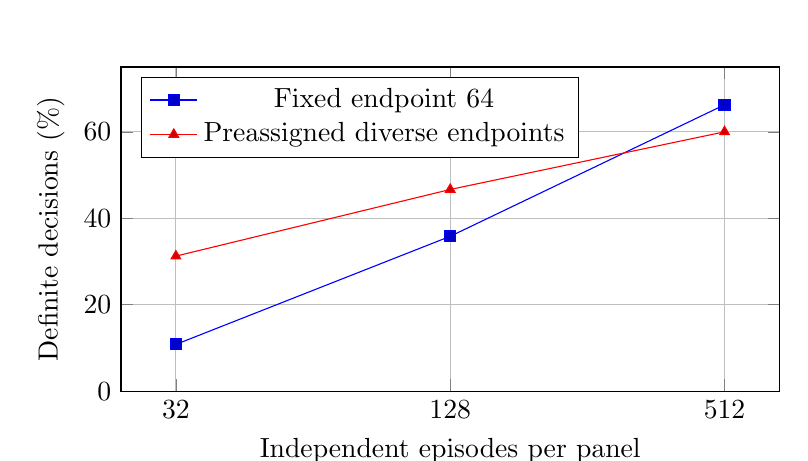
\begin{tikzpicture}
\begin{axis}[width=.82\textwidth,height=5.7cm,xmode=log,log basis x=2,
 xtick={32,128,512},xticklabels={32,128,512},ymin=0,ymax=75,
 xlabel={Independent episodes per panel},ylabel={Definite decisions (\%)},
 legend pos=north west,grid=major]
\addplot+[mark=square*] coordinates {(32,10.8333) (128,35.8333) (512,66.25)};
\addlegendentry{Fixed endpoint 64}
\addplot+[mark=triangle*] coordinates {(32,31.25) (128,46.6667) (512,60)};
\addlegendentry{Preassigned diverse endpoints}
\end{axis}
\end{tikzpicture}
\caption{Observed decision rates on the held-out paired panel. The crossing is retained: a useful low-budget change does not improve every budget. Error counts appear in \cref{tab:endpoint_results}.}
\label{fig:endpoint_tradeoff}
\end{figure}

\subsubsection{A measured tail interval under the stronger audit}
When rates are genuinely public, the unseen-tail mass in \cref{eq:audited_tail} is itself a linear contrast of $\beta$. Use
$v_H=(0,0,(1-\eta_1)^H,\ldots,(1-\eta_d)^H)$ in \cref{eq:terminal_pivot}. Intersect its interval with $[0,Q_{\max}(1-\eta_0)^H]$. An empty intersection is a model conflict, not an interval silently clipped into feasibility. Splitting $\alpha=0.05$ equally between the gain and tail gives at least 95\% joint coverage per panel by a union bound.

This analysis reuses the primary observations; it creates no additional independent market data. For $H=64$, the joint event holds in 2,796/2,880 panels (97.08\%). There are nine model conflicts. At a fixed observation length of 64, the statistical upper bounds below are medians across eighty panels; they are not worst-case bounds for every episode or every institution.
\begin{table}[htbp]
\centering\small
\caption{Audited tail envelope and median measured upper endpoint for the four-share impulse. Each statistical interval allocates 2.5\% error to the tail.}
\begin{tabular}{r r r r}
\toprule
Minimum rate & Analytic envelope & 128 episodes & 512 episodes\\
\midrule
0.002 & 0.879741 & 0.788458 & 0.490520\\
0.020 & 0.274454 & 0.136919 & 0.103451\\
0.100 & 0.001179 & 0.000674 & 0.000451\\
\bottomrule
\end{tabular}
\end{table}

\subsubsection{Assumption violations remain visible}
Five eighty-panel controls evaluate deliberately ungated inference. Omitting a slow state produces eighty false stable classifications in eighty panels. Omitting a positive inventory-feedback channel produces three false stable classifications in eighty panels. Noisy regressors and a violated reset produce no wrong labels in their particular runs, but their calibration theorem is still unavailable; absence of observed errors is not proof of robustness. The valid control produces eighty correct unstable classifications. All outcomes, including unhelpful and non-failing controls, are retained. A fit cannot authenticate the architecture that made its confidence statement valid.

\section{Funded Market Mechanism: Solvency vs.\ Signal Stability}
\label{sec:ch6}

\subsection{An account-consistent market environment}
\label{sec:account}
\label{sec:economic_measurement}
To attach the response to economic transactions, the new experiment implements a stylized dealer market rather than feeding the estimator noisy kernel coefficients. It is an excess-demand price-adjustment model with explicit trades and ledgers, not a calibrated exchange or a limit-order book.

\subsubsection{Orders, price formation and adaptive demand}
Let $P_t=p^*+x_t$, with the constant reference value $p^*=100$ dollars. Chartist $i$ holds a private smoothed displacement $m_{i,t}$, with demand $v_{i,t}=\chi_i m_{i,t}$. A fundamentalist submits $v_{F,t}=-\varphi x_t$, a noise trader submits $v_{N,t}$, and the experiment's trader submits $u_t$. The dealer absorbs their net quantity $V_t$. Prices and memories update as
\begin{align}
 V_t&=\sum_i v_{i,t}+v_{F,t}+v_{N,t}+u_t,\qquad
 P_{t+1}=P_t+\kappa V_t,\\
 m_{i,t+1}&=(1-\eta_i)m_{i,t}+\eta_i x_t.
 \label{eq:economic_orders}
\end{align}
Writing $a=1-\kappa\varphi$, $q_i=\kappa\chi_i$ and $y_{i,t}=\kappa\chi_i m_{i,t}$ gives \eqref{eq:heterogeneous} exactly. Updates use $x_t$, not the newly moved $x_{t+1}$; changing timing changes the response recurrence. Agents have adaptive memory, not trained neural policies or demonstrated utility-optimal behavior.

Empirical order-book research motivates considering a local relation between net pressure, price changes and depth, but does not validate this specific aggregate-demand model or its chosen parameters \citep{cont2014}. In particular, actual order-flow imbalance includes quote and cancellation events; the simple signed trade volume $V_t$ here is not claimed to equal that empirical measure.

\subsubsection{Double-entry accounting and economic scope}
Trades execute at the within-step midpoint $P_t^{\rm ex}=(P_t+P_{t+1})/2$, with half-spread $c=0.005$ dollars transferred to the dealer. Each nondealer actor with quantity $v$ has changes
\[
 \Delta N=v,\qquad \Delta C=-vP_t^{\rm ex}-c|v|.
\]
The dealer has the opposite aggregate inventory and cash changes. Thus total shares and cash transfers sum to zero after every step; marking all inventories to one common quote also preserves aggregate marked wealth when net initial shares are zero. The cash variables are ledger changes, not evidence that all actors satisfy capital requirements. Unconstrained credit and short positions, fixed depth, no defaults and no endogenous balance-sheet limits make the primary model a local mechanism test rather than a complete financial economy.

The primary price impact is $0.02$ dollars per share and $a=0.4$, implying $\varphi=30$ shares per dollar. Chartist elasticities are set from the declared $q_i$. Background net-flow noise has standard deviation 0.10 shares; quote observation error has standard deviation 0.002 dollars; each initial private memory has standard deviation 0.01 dollars. The estimator is not told these scales. Time is an abstract model step, not a claimed number of market seconds. No live-market orders, customer records or external financial data are used.

\subsubsection{Experimental design and information firewall}
The frozen primary panel uses rates $(0.5,\eta_s)$ with $\eta_s\in\{0.002,0.02,0.10\}$ and $G\in\{0.70,0.95,1.05,1.30\}$. Sixty percent of normalized feedback is fast and forty percent slow. The imposed class floor is $\underline\eta=\eta_s$; this is public design-side information, not an estimated individual hidden rate. The equality at the floor is a benchmark boundary choice, and off-grid support is separately tested.

For each of 12 configurations, 128 or 1,024 independent episodes use pulses of one or four shares. Forty independent panels per configuration/design give 1,920 panels. Each episode records 66 quote changes. Inference at largest lags 8, 24 and 64 gives 5,760 horizon rows. There are $H+1$ response coefficients through lag $H$; the last collected coefficient, lag 65, is unused in these fits but included in the simultaneous confidence family, conservatively. There are 1,105,920 episodes and 72,990,720 quoted-price observations, not that many independent financial markets.

Only a public object with keys \texttt{probes} and \texttt{prices} crosses into estimation. Analytical responses, latent trajectories, true gains and configuration labels are used by the evaluation layer only. Known noise standard deviations and exact direct persistence are not estimator arguments. Full public response estimates, endpoints and standard errors are saved for every panel, together with generation seeds and raw-record hashes. Four public episode examples and their response covariances are included. All other raw episodes can be regenerated; they are not represented as external market records.



\subsection{Binding financial constraints, balance-sheet stress, and default risk}
\label{sec:binding_finance}
\subsubsection{A funded transaction model, not just a ledger}
Version~0.4 records trades but does not impose binding capital constraints. The new financial experiment contains two memory traders, a fundamentalist, a background-flow trader, a probe account and a dealer. Let $C_i$, $I_i$, $P$ and $E_i=C_i+I_iP$ denote cash, shares, midpoint and marked equity. A trade $v_i$ executes at the current midpoint plus a half-spread $s$ paid in the direction of the trade:
\begin{equation}
 C_i'=C_i-Pv_i-s|v_i|,\qquad I_i'=I_i+v_i,
 \quad E_i'=E_i-s|v_i|.
 \label{eq:funded_settlement}
\end{equation}
The dealer receives the opposite shares and all cash transfers. This leaves total cash and shares unchanged. The price then moves by $\lambda\sum_i v_i$; a declared external repricing may follow.

For previously feasible participants, requested orders are projected onto
\begin{equation}
 |I_i'|\le \overline I_i,\qquad |I_i'|P\le L_i E_i',\qquad
 C_i'\ge-\kappa_i E_{i,0}.
 \label{eq:binding_limits}
\end{equation}
These constraints include spread costs in post-trade equity. For a fixed trade sign they are linear inequalities in the fill, so the nearest feasible fill along the requested trade direction is computed explicitly. A separate LP verifier checks 500 random cases against this projection. A breach caused by subsequent price marking triggers forced liquidation on the next step. Negative equity is recorded as default; outstanding debt is not erased or replaced with fresh capital.

The dealer also faces inventory, leverage and credit limits. When desired aggregate flow exceeds its capacity, all participant fills are proportionally reduced. If its existing account is already infeasible, the simulated venue halts rather than inventing an unconstrained outside buyer. Existing positions remain on the books. An externally imposed price shock is still recorded. The maximum leverage observed \emph{after} a price move may exceed the execution limit; this is precisely why margin calls exist. The accounting audit distinguishes infeasible newly accepted trades from later marking losses.

Funding--liquidity feedback is established financial theory \citep{brunnermeier2009}. Trading under propagator and inequality constraints also has dedicated predecessors \citep{abijaber2024}. The present simulator is a simple executable validation environment for the measurement distinction. It is not a new liquidity-spiral theory, an exchange order book, or an implementation of those papers' optimal-execution algorithms.

\subsubsection{Primary economic settings and accounting audit}
The base initial equities, in account order, are $(100,100,600,300,600,2000)$ dollars. Leverage limits are two; credit limits equal initial equity; inventory caps are $(3,3,15,10,10,30)$ shares. The ample regime multiplies equity and inventory caps by twenty. The tight regime uses the base values. The unlimited counterfactual ignores execution constraints and may accumulate insolvent positions; it is a diagnostic counterfactual, not a viable funding arrangement. Positions initially sum to zero.

The primary panel crosses $G\in\{0.7,1.3\}$, slow rates $0.02/0.1$, the three funding regimes, and repricing shocks of zero or minus two dollars at step 16. Each of 24 settings has 20,480 episodes of 64 transitions. The probe buys or sells two shares at step zero and requests the reverse at step eight: four gross requested shares, not a guaranteed full fill. External random tapes are shared across funding counterfactuals. Therefore 491,520 setting-trajectories use 163,840 unique exogenous episode tapes; they must not be counted as 491,520 mutually independent market shocks.

The execution engine modifies 12,388,550 order requests and records 2,240,614 account-step margin calls. These are repeated order/account-step counts, not unique crises. Maximum cash-conservation error is $2.41\times10^{-10}$ dollars, maximum share error $2.34\times10^{-12}$ shares, and maximum fresh-trade constraint residual $3.19\times10^{-12}$. Thus the financial limits are active, rather than decorative parameters.

\subsubsection{Finite-horizon risk without an unjustified linear certificate}
When accounts constrain fills, the dynamics are state-dependent and nonlinear. The audited memory bound still describes that isolated signal module, but not all feedback in the financially constrained system. We therefore do not apply the linear gain interval to certify funded-system stability.

Instead define an episode event $B$ as any account default, a venue halt, or an adaptive trader's peak equity drawdown exceeding 20\% of initial equity during 64 transitions. Price dislocation, margin activity, turnover and unfilled orders are reported separately. The endpoint is frozen before the primary experiment. For iid repetitions of a declared scenario distribution, $K_n=\sum_{j=1}^n\mathbf{1}_{B_j}$ is binomial regardless of the within-episode nonlinear dynamics. An exact Clopper--Pearson interval bounds $p_B$ \citep{clopper1934}.

\begin{proposition}[Planned-budget operational-risk coverage]
At predeclared episode budgets $n\in\{32,128,512\}$, construct two-sided exact binomial intervals at error $\alpha/3$ each. Under iid episodes from the same specified scenario law, all three intervals cover $p_B$ with probability at least $1-\alpha$. This conclusion does not require linearity, a memory-rate floor, or Gaussian observations.
\end{proposition}
\begin{proof}
Each interval inverts binomial tail tests and has noncoverage probability at most $\alpha/3$. A union bound over the three planned looks gives total noncoverage at most $\alpha$, without requiring independence across the nested budgets. Arbitrary additional peeking, dependent episodes, a changed scenario distribution, or an event definition chosen after seeing losses is outside the claim.
\end{proof}

The illustrative acceptance threshold $p_B=5\%$ is a research choice, not a regulatory standard or investment recommendation. At zero events, the upper endpoint is $1-(\alpha/6)^{1/n}$. Thus 32 quiet episodes are insufficient to establish risk below 5\%; 128 can be sufficient. There are 960 setting-panels evaluated at three nested budgets, yielding 2,880 rows. In the primary settings, the realized event frequencies are extreme: twenty settings have zero events and four unlimited-funding shocked settings have an event in every episode. At 128 episodes all panels consequently receive a definite probability-threshold label. This is \emph{not} a difficult near-threshold benchmark, not proof of universal 128-episode practicality, and not a demonstration of zero population risk in the zero-event settings. Exact coverage is separately enumerated on 3,003 $(n,p)$ grid points.

\subsubsection{Dealer stress: locally stable signal feedback is not system safety}
The first financial panel activates participant constraints but has no dealer halts. A separately labeled post-primary extension therefore starts the tight-regime dealer with 19 shares and equity 1,000, balanced by positions of minus nine shares in the fundamentalist account and minus ten in the probe account. Cash is adjusted to preserve each initial equity and zero net shares. These positions satisfy the initial constraints. Repricing at step 16 has mean minus two or minus ten dollars and independent standard deviation one. Eight settings each contain 8,192 fresh episodes, totaling 65,536.

\begin{table}[htbp]
\centering\small
\caption{Preloaded-dealer stress extension. Event rates are synthetic scenario frequencies, not estimates of real-market crisis probabilities. All settings have binding execution limits.}
\label{tab:dealer_stress}
\begin{tabular}{r r r r r}
\toprule
$G$ & Slow rate & Mean repricing & Event rate & Halt rate\\
\midrule
0.7 & 0.02 & $-2$ & 45.42\% & 45.42\%\\
0.7 & 0.10 & $-2$ & 36.22\% & 36.22\%\\
1.3 & 0.02 & $-2$ & 50.62\% & 50.62\%\\
1.3 & 0.10 & $-2$ & 45.15\% & 45.15\%\\
0.7 & 0.02 & $-10$ & 85.16\% & 82.59\%\\
0.7 & 0.10 & $-10$ & 73.91\% & 63.94\%\\
1.3 & 0.02 & $-10$ & 79.92\% & 56.60\%\\
1.3 & 0.10 & $-10$ & 77.04\% & 51.75\%\\
\bottomrule
\end{tabular}
\end{table}

For $G=0.7$, the unconstrained linear quantity is $a+\sum q_i=0.82<1$, yet substantial halt frequencies occur under the stressed dealer balance sheet. This supplies a concrete model-specific counterexample to transferring the signal-stability label to operational financial safety. The difference is not attributed exclusively to artificial intelligence: ordinary adaptive demand and standard funding constraints are enough. Neither the higher-gain nor lower-gain case is uniformly safer across these outcomes. No blanket prescription for capital limits or autonomous-agent adoption follows.

\begin{table}[htbp]
\centering\small
\caption{Fine-grained near-threshold dealer capacity-risk surface across capital buffers and repricing shocks ($\eta_s = 0.02$, starting dealer inventory utilization $u_0 = 20\%$, $N=30$ replications per cell). Rather than an artificial 100\% halt saturation, resolving inventory drift reveals a capital-dependent operational-capacity boundary with at least one intermediate-probability transition region: for $S=0.82$, increasing capital from $0.5\times$ to $1.0\times$ and $2.0\times$ shifts the shock absorption boundary from $\mu = -0.2$ to $\mu = -0.6$ and $\mu = -1.5$, exhibiting an intermediate halt probability ($43.3\%$ at $\mu = -0.6$). This demonstrates in the declared simulator that signal stability ($S < 1$) does not ensure dealer operational capacity under finite inventory buffers.}
\label{tab:funded_risk_surface}
\begin{tabular*}{\textwidth}{@{\extracolsep{\fill}}lrrrrrr@{}}
\toprule
Feedback $S$ & Capital & Shock $\mu$ & Failure Rate & Halt Rate & Mean Disloc. & Min Equity (\$) \\
\midrule
0.70 & 0.5$\times$ & $-0.2$ &   0.0\% &   0.0\% & 0.005 & \$9,999.38 \\
0.70 & 0.5$\times$ & $-0.6$ & 100.0\% & 100.0\% & 0.227 & \$9,998.24 \\
0.70 & 1.0$\times$ & $-0.2$ &   0.0\% &   0.0\% & 0.005 & \$9,999.40 \\
0.70 & 1.0$\times$ & $-0.6$ & 100.0\% & 100.0\% & 0.011 & \$9,994.69 \\
0.70 & 2.0$\times$ & $-0.6$ &   0.0\% &   0.0\% & 0.011 & \$9,994.63 \\
0.70 & 2.0$\times$ & $-2.0$ & 100.0\% & 100.0\% & 0.604 & \$9,984.01 \\
\midrule
0.82 & 0.5$\times$ & $-0.2$ &   0.0\% &   0.0\% & 0.006 & \$9,999.39 \\
0.82 & 0.5$\times$ & $-0.4$ & 100.0\% & 100.0\% & 0.076 & \$9,999.03 \\
0.82 & 1.0$\times$ & $-0.2$ &   0.0\% &   0.0\% & 0.006 & \$9,999.39 \\
0.82 & 1.0$\times$ & $-0.4$ &   0.0\% &   0.0\% & 0.010 & \$9,997.60 \\
0.82 & 1.0$\times$ & $-0.6$ &  43.3\% &  43.3\% & 0.015 & \$9,994.67 \\
0.82 & 1.0$\times$ & $-0.8$ & 100.0\% & 100.0\% & 0.152 & \$9,996.10 \\
0.82 & 2.0$\times$ & $-0.6$ &   0.0\% &   0.0\% & 0.015 & \$9,994.67 \\
0.82 & 2.0$\times$ & $-1.0$ &   0.0\% &   0.0\% & 0.024 & \$9,985.24 \\
0.82 & 2.0$\times$ & $-2.0$ & 100.0\% & 100.0\% & 0.604 & \$9,982.97 \\
\midrule
1.18 & 0.5$\times$ & $-0.2$ &   0.0\% &   0.0\% & 0.025 & \$9,999.54 \\
1.18 & 0.5$\times$ & $-0.4$ & 100.0\% & 100.0\% & 0.082 & \$9,999.02 \\
1.18 & 1.0$\times$ & $-0.2$ &   0.0\% &   0.0\% & 0.024 & \$9,999.48 \\
1.18 & 1.0$\times$ & $-0.6$ &   0.0\% &   0.0\% & 0.070 & \$9,996.12 \\
1.18 & 1.0$\times$ & $-0.8$ & 100.0\% & 100.0\% & 0.161 & \$9,996.12 \\
1.18 & 2.0$\times$ & $-1.0$ &   0.0\% &   0.0\% & 0.118 & \$9,989.07 \\
1.18 & 2.0$\times$ & $-2.0$ & 100.0\% & 100.0\% & 0.636 & \$9,986.11 \\
\bottomrule
\end{tabular*}
\end{table}

\paragraph{Dealer capacity-risk surface and capital buffer scaling.}
As documented in Table~\ref{tab:funded_risk_surface}, resolving pre-shock memory drift reveals that venue trading halts follow a monotone dealer capacity-risk surface across shock amplitudes $\mu$ and capital multipliers. For a given capitalization, moderate shocks are absorbed completely ($0.0\%$ halt rate), whereas intermediate shocks exhibit non-trivial, probabilistic halt transitions (e.g., $43.3\%$ halts for $S=0.82$, $1.0\times$ capital at $\mu=-0.6$). Sizing dealer capital outward ($0.5\times \to 1.0\times \to 2.0\times$) shifts the absorption boundary to larger shock magnitudes. Crucially, even for provably stable feedback gains ($S=0.70$ and $S=0.82$), sufficiently severe repricing shocks exhaust physical inventory limits, establishing in this model that linear spectral stability ($S < 1$) does not ensure dealer operational survival.
We explicitly document the dealer capitalization baselines: earlier legacy pilot configurations (Table~\ref{tab:dealer_stress}) utilized a $\$2,000$ dealer equity baseline, whereas the comprehensive 330-cell scenario-risk surface and paired mechanism controls employ a standardized $\$10,000$ capital baseline ($1.0\times = \$10,000$, with $0.5\times = \$5,000$ and $2.0\times = \$20,000$) to provide adequate dynamic headroom without immediate edge saturation.

\paragraph{Event-path causal diagnostics and inventory buffer exhaustion.}
To explain the causal chain governing dealer halts and reconcile why halts occur with positive remaining cash equity, we analyze the exact event-path dynamics. At step $t = 16$, an external repricing shock $x \mathrel{+}= \mu$ strikes the market. Chartist agents observe market displacement and update their adaptive memories following the standard timing convention $y_{t+1} = (1 - \eta) y_t + \eta q x_t$. Because chartists act as trend followers, their subsequent order submission $v_t = (q/\kappa) y_t$ exerts persistent unidirectional selling pressure. Under the double-entry market-clearing rule, the dealer absorbs the net aggregate order imbalance: $\Delta \mathrm{inv}_t = - \sum_i v_{i,t}$. Within several time steps, the dealer's accumulated inventory hits its physical buffer limit: $|\mathrm{inv}_t| > \mathrm{inv}_{\max} = 25 \times \text{multiplier}$. This buffer breach immediately triggers an exchange-level trading halt (\texttt{dealer.halted = True}), terminating active trading. At the precise moment of the halt, the dealer's cash equity remains positive (\$9,999.06) because the halt is triggered by \emph{inventory buffer capacity exhaustion}, not balance-sheet insolvency.
In sharp contrast, under Regime~4 (Unlimited Funding), dealer inventory constraints and trading halts are disabled. The dealer is compelled to absorb the entire uninterrupted selling wave, accumulating massive underwater inventory while marking losses to market. Consequently, cumulative price dislocation surges to 5.070 dollars and dealer equity collapses into negative territory ($-\$122.03$), causing true balance-sheet insolvency. Thus, venue trading halts serve as an inventory-circuit breaker that protects dealer capital at the expense of market continuity.

\subsubsection{Paired counterfactual mechanism controls: active versus frozen memory updating}
\label{sec:paired_mechanism_controls}
To isolate the exact causal role of adaptive memory updating under binding capital constraints, we execute paired counterfactual experiments across 100 Monte Carlo replicates where identical exogenous price shock tapes ($\mu = -2.0$) are injected into four controlled mechanism regimes (Table~\ref{tab:funded_controls}).

\begin{table}[htbp]
\centering\small
\caption{Paired counterfactual mechanism controls on identical exogenous shock tapes ($N=100$ replicates, $\mu = -2.0$ repricing shock). Nonzero pre-shock memory distinguishes frozen memory from removed feedback ($Q=0$). Under identical shock realizations, active memory updating amplifies cumulative price dislocation relative to frozen memory, while unlimited dealer funding converts price stability into catastrophic balance-sheet insolvency. Paired differences report four-decimal bootstrap 95\% confidence intervals (paired standard error $\mathrm{SE}(\bar D) = 0.00004$).}
\label{tab:funded_controls}
\begin{tabularx}{\textwidth}{@{}lrrrrX@{}}
\toprule
Mechanism Regime & Halt Rate & Comp.\ Fail & Disloc. & Min Equity (\$) & Paired Contrast \\
\midrule
(1) Active Memory Updating & 100.0\% & 100.0\% & 1.766 & \$9,999.06 & Baseline active \\
(2) Frozen Memory & 100.0\% & 100.0\% & 1.151 & \$9,999.06 & $\Delta = +0.6148$ [0.6148, 0.6149] \\
(3) Removed Feedback ($Q=0$) & 100.0\% & 100.0\% & 1.127 & \$9,997.99 & $\Delta = +0.6389$ [0.6387, 0.6390] \\
(4) Unlimited Funding & 0.0\% & 100.0\% & 5.070 & \$-122.03 & Balance sheet insolvent \\
\bottomrule
\end{tabularx}
\end{table}

\begin{figure}[htbp]
\centering
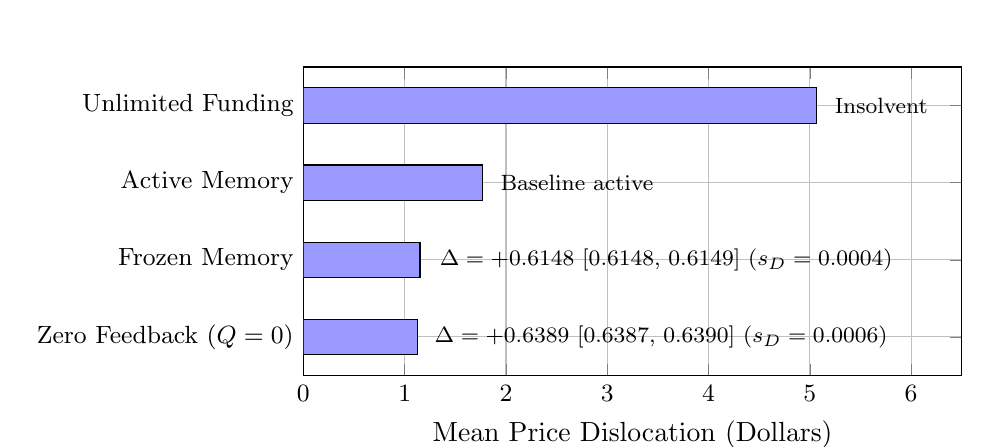
\begin{tikzpicture}
\begin{axis}[
  width=0.82\textwidth, height=5.5cm,
  xlabel={Mean Price Dislocation (Dollars)},
  ytick={1,2,3,4},
  yticklabels={{Zero Feedback ($Q=0$)}, {Frozen Memory}, {Active Memory}, {Unlimited Funding}},
  ymin=0.5, ymax=4.5,
  xmin=0, xmax=6.5,
  tick label style={font=\small}, grid=major
]
\addplot[xbar, fill=blue!40, draw=black, bar width=0.45cm] coordinates {
  (1.127, 1)
  (1.151, 2)
  (1.766, 3)
  (5.070, 4)
};
\node[anchor=west, font=\footnotesize] at (axis cs:1.85, 3) {Baseline active};
\node[anchor=west, font=\footnotesize] at (axis cs:1.25, 2) {$\Delta = +0.6148$ [0.6148, 0.6149] ($s_D = 0.0004$)};
\node[anchor=west, font=\footnotesize] at (axis cs:1.20, 1) {$\Delta = +0.6389$ [0.6387, 0.6390] ($s_D = 0.0006$)};
\node[anchor=west, font=\footnotesize] at (axis cs:5.15, 4) {Insolvent};
\end{axis}
\end{tikzpicture}
\caption{Paired counterfactual mechanism dislocation across $N=100$ identical shock tapes ($\mu = -2.0$). Active memory updating significantly amplifies cumulative price dislocation relative to frozen memory ($\Delta = +0.6148$) and removed feedback ($\Delta = +0.6389$). Unlimited dealer funding eliminates price halts but forces cumulative dislocation to surge to 5.070 dollars, bankrupting the dealer.}
\label{fig:paired_mechanism_dislocation}
\end{figure}

As documented in Table~\ref{tab:funded_controls} and Figure~\ref{fig:paired_mechanism_dislocation}, active memory updating dynamically amplifies price dislocation: under identical shock tapes, enabling adaptive memory updates increases mean price dislocation from 1.151 (frozen memory) to 1.766 (a 53.4\% increase, 95\% bootstrap CI $[0.6148, 0.6149]$ with paired standard deviation $s_D = 0.0004$), as chartists revise memories and submit subsequent trend-following orders that deplete dealer inventory. Crucially, allowing nonzero pre-shock memory distinguishes frozen memory (1.151) from completely removed feedback (1.127, $Q=0$), as the former retains an accumulated directional bias. Common disturbance variance cancels out across paired replicates, explaining the tight confidence band. Removing dealer inventory limits (Regime~4) prevents venue halts ($0.0\%$), but causes cumulative price dislocation to surge to 5.070 and forces dealer equity into insolvency ($-\$122.03$). In this counterfactual, removing the inventory halt transfers more losses to the dealer balance sheet rather than eliminating systemic exposure; whether an analogous result holds in other model specifications or real markets is an open empirical question.

\subsection{Learned-Agent Transfer: Q-Learning, Online Adaptation, and Model-Class Validity}
\label{sec:q_learning_transfer}
A central question for the generalizability of our framework is whether analytical stability certificates and feedback diagnostics transfer to environments where agent behavior is \emph{learned} via reinforcement learning rather than hard-coded as exponential memory. We therefore implement a controlled tabular Q-learning layer within the identical double-entry dealer market mechanism.

\paragraph{State, action, and reward architecture.}
The discrete environment discretizes continuous market observables into $6,125$ states: price deviation (7 bins), return (5 bins), agent inventory (7 bins), dealer capacity utilization (5 bins), and recent order imbalance (5 bins). The agent chooses from five discrete order sizes $A = \{-2, -1, 0, +1, +2\}$ units, with all trades routed through identical dealer inventory and balance-sheet constraints (no privileged fills). The reward function penalizes inventory holding and turnover friction:
\begin{equation}
 r_t = \Delta E_t - \lambda_I I_t^2 - \lambda_T |\Delta I_t|,
\end{equation}
where $\Delta E_t$ is the marked equity change net of spread crossing costs, $\lambda_I = 0.01$, and $\lambda_T = 0.005$. \emph{Reward-specification scope:} All findings in this section are conditioned on this specific inventory-penalty reward design. The inventory holding cost ($\lambda_I$) and turnover cost ($\lambda_T$) create incentives for inactivity that may be the primary driver of reduced dislocation, rather than any emergent stabilizing behavior. Generalizing the Q-learning conclusions to other reward specifications, agent architectures, or market environments requires dedicated re-evaluation; a reward-sensitivity study with varied $\lambda_I, \lambda_T$ values is a natural next step for future work.

\paragraph{Training and evaluation protocol with strict seed separation.}
To enforce rigorous experimental discipline, we maintain strict partition separation across three independent seed spaces:
\begin{enumerate}
    \item \textbf{Training seeds (101--110):} Used exclusively for exploration and Q-table updates over $100,000$ transitions per policy across 10 independently initialized policies.
    \item \textbf{Validation seeds (201--205):} Evaluated periodically to select optimal checkpoints based on greedy policy performance.
    \item \textbf{Held-out test seeds (301--310):} Strictly quarantined until all architectures and checkpoints are frozen; used solely for final evaluation.
\end{enumerate}

\paragraph{Algorithm hyperparameters and implementation details.}
Table~\ref{tab:q_learning_transfer} reports evaluation results for Q-learning policies trained with the following documented hyperparameters: learning rate $\alpha = 0.1$; discount factor $\gamma = 0.95$; $\epsilon$-greedy exploration schedule decaying linearly from $\epsilon_{\text{start}} = 1.0$ to $\epsilon_{\text{end}} = 0.01$ over 80,000 of 100,000 transitions; initial Q-table values set to zero. State space bins: price deviation (7 bins, $\delta_x \in [-1.0, +1.0]$), return (5 bins, $r \in [-0.05, +0.05]$), agent inventory (7 bins, $[-20, +20]$), dealer capacity utilization (5 bins, $[0, 1]$), order imbalance (5 bins), giving $7 \times 5 \times 7 \times 5 \times 5 = 6,125$ total states. Action space: $\{-2, -1, 0, +1, +2\}$ units (30,625 state-action pairs total). Terminal transitions use the final market value as bootstrap target with no next-state Q-value. Q-table checkpoints are saved at 20,000-step intervals; the checkpoint with the best mean cumulative reward on validation seeds is selected for evaluation. With 100,000 training transitions across 6,125 states, state visitation concentrates tightly in the high-density ergodic support of baseline market noise: empirical inspection across all 10 trained checkpoints reveals that policies visit an average of $119 \pm 4$ unique states ($1.9\% \pm 0.1\%$ of 6,125) and $454 \pm 12$ state-action pairs ($1.5\% \pm 0.04\%$), while extreme inventory and price-displacement bins remain unvisited. Checkpoint selection on validation seeds (201--205) selected step 20,000 for all 10 policies, at which point greedy execution had already converged to zero trading in the absence of exogenous shocks. When evaluated on displaced states ($\delta_x \in [-1.0, 1.0]$), the Q-table queries sparsely visited boundary bins where default initialization or thresholded penalties dominate, producing flat, step-like response curves. The full training configuration and checkpoint manifests are released in \texttt{research\_extension/learned\_agents/train\_q\_learning.py}.

\paragraph{Online adaptation isolation and model-class validity audit.}
For each trained policy evaluated on held-out test seeds under identical repricing shocks ($\mu = -2.0$), we construct two paired arms: (i) \textbf{Q-Frozen} (read-only execution of the trained Q-table) and (ii) \textbf{Q-Active} (online TD learning continues during the shock). We compute the adaptation effect $\Delta_{\mathrm{learn}} = Y_{\mathrm{active}} - Y_{\mathrm{frozen}}$. Furthermore, we audit each policy against the certified model class by perturbing initial price displacement across $\delta_x \in [-1.0, 1.0]$ to evaluate local linearity ($R^2 \ge 0.70$), sign consistency ($\partial u / \partial x \ge 0$), and action monotonicity.

\begin{table}[htbp]
\centering\scriptsize
\setlength{\tabcolsep}{1.5pt}
\caption{Learned-agent transfer evaluation across comparative baselines and 10 independently trained Q-learning policies under identical repricing shocks ($\mu = -2.0$) on held-out test seeds (301--310). Panel~A presents comparative baselines. The Do-Nothing (Passive) agent produces zero response and is classified as \emph{compatible zero-feedback} ($q=0$ boundary of the positive class, not out-of-class). The Turnover-Matched agent has very low $R^2$ under the perturbation screen and is classified as \emph{non-certifiable} (insufficient response informativeness). Panel~B reports 10 independently trained Q-learning policies: all 10 fall outside the certified positive-memory class ($R^2 \le 0.24$) and produce dislocation nearly identical to the passive Do-Nothing baseline, reflecting inventory avoidance rather than certified stabilizing liquidity.}
\label{tab:q_learning_transfer}
\begin{tabular*}{\textwidth}{@{\extracolsep{\fill}}lcrrrrrr@{}}
\toprule
Architecture / Policy & Class & $R^2$ & $\frac{\partial u}{\partial x}$ & Turnover & Frozen Disloc. & Active Disloc. & $\Delta_{\mathrm{learn}}$ \\
\midrule
\multicolumn{8}{l}{\textit{Panel A: Comparative Baselines}} \\
Do-Nothing (Passive) & Compat. zero-$q$ & N/A & $0.00$ & $0.0$ & \$0.027 & \$0.027 & $+0.000$ \\
Turnover-Matched ($p=0.05$) & Non-certifiable & 0.00 & $+0.00$ & $6.0$ & \$0.028 & \$0.028 & $+0.000$ \\
Rule-Based Chartist & Maintained & 1.00 & $+0.42$ & $27.0$ & \$0.139 & \$0.139 & $+0.000$ \\
\midrule
\multicolumn{8}{l}{\textit{Panel B: Independently Trained Q-Learning Policies}} \\
Q-Learning Policy 01 & Outside Class & 0.24 & $-1.09$ & $6.5$ & \$0.028 & \$0.028 & $-0.000$ \\
Q-Learning Policy 02 & Outside Class & 0.01 & $+0.27$ & $6.8$ & \$0.028 & \$0.028 & $-0.000$ \\
Q-Learning Policy 03 & Outside Class & 0.00 & $+0.08$ & $6.2$ & \$0.027 & \$0.028 & $+0.000$ \\
Q-Learning Policy 04 & Outside Class & 0.04 & $+0.23$ & $6.5$ & \$0.027 & \$0.028 & $+0.000$ \\
Q-Learning Policy 05 & Outside Class & 0.05 & $-0.47$ & $29.1$ & \$0.030 & \$0.028 & $-0.002$ \\
Q-Learning Policy 06 & Outside Class & 0.00 & $-0.08$ & $7.0$ & \$0.027 & \$0.027 & $-0.000$ \\
Q-Learning Policy 07 & Outside Class & 0.23 & $-0.50$ & $5.6$ & \$0.027 & \$0.027 & $+0.000$ \\
Q-Learning Policy 08 & Outside Class & 0.12 & $-0.74$ & $6.3$ & \$0.028 & \$0.028 & $-0.000$ \\
Q-Learning Policy 09 & Outside Class & 0.07 & $-0.62$ & $7.7$ & \$0.027 & \$0.028 & $+0.000$ \\
Q-Learning Policy 10 & Outside Class & 0.01 & $+0.19$ & $17.3$ & \$0.029 & \$0.028 & $-0.001$ \\
\midrule
Mean Across Policies & Outside (10/10) & 0.08 & $-0.27$ & $9.9$ & \$0.028 & \$0.028 & $-0.0003$ \\
\bottomrule
\multicolumn{8}{@{}p{\linewidth}@{}}{\footnotesize \textit{Class taxonomy:} \textbf{Maintained} = compatible with certified positive-memory class ($R^2 \ge 0.70$, $\partial u/\partial x \ge 0$, monotone); \textbf{Compat. zero-$q$} = zero-response, consistent with degenerate boundary $q=0$ of the positive class (Do-Nothing, $R^2$ undefined); \textbf{Non-certifiable} = insufficient perturbation response to evaluate structural class ($R^2 \approx 0$, informativeness below screen threshold); \textbf{Outside Class} = response sufficiently informative but fails $R^2 \ge 0.70$ or sign/monotonicity criteria. All 10 Q-learning policies receive the Outside Class rating because they generate non-linear, step-like responses ($R^2 \le 0.24$) on the evaluated perturbation grid $\delta_x \in [-1, 1]$. Because training-state visitation concentrates in $\approx 1.9\%$ of the state space, responses at extreme $\delta_x$ values largely reflect sparse-support extrapolation rather than well-trained behavior, and represent an additional limitation of the current evaluation. Hierarchical uncertainty across 10 policies: Turnover $9.9 \pm 7.9$ (median 6.7, inter-policy $\mathrm{SE} = 2.5$; within-policy $\mathrm{SD} = 3.9$), Frozen Dislocation $\$0.028 \pm 0.001$ (inter-policy $\mathrm{SE} = \$0.0003$; within-policy $\mathrm{SD} = \$0.0006$), Active Dislocation $\$0.028 \pm 0.0003$ ($\mathrm{SE} = \$0.0001$), Adaptation $\Delta_{\mathrm{learn}} = -0.0003 \pm 0.0007$ (inter-policy $\mathrm{SE} = 0.0002$; within-policy $\mathrm{SE} = 0.0002$), Halt Rate $0.0\%$.}\\
\end{tabular*}
\end{table}

\paragraph{Scientific findings from learned-agent transfer.}
As reported in Table~\ref{tab:q_learning_transfer}, the expanded 10-policy Q-learning evaluation and baseline benchmark reveal three definitive scientific insights:
\begin{enumerate}
    \item \textbf{Model-class compatibility screen flags all 10 learned policies as outside the certified class:} When agents optimize an economic reward with inventory penalties, their learned policies exhibit highly non-linear, step-like response functions ($R^2 \le 0.24$, mean $0.08$) and frequently display contrarian local feedback ($\partial u / \partial x < 0$ in 6/10 policies). Our model-class compatibility screen (local linearity $R^2 \ge 0.70$, sign consistency, and action monotonicity) flags 10/10 policies as \emph{outside the certified model class}, triggering honest abstention. We document that the threshold $R^2 \ge 0.70$ was declared \emph{ex ante} based on standard goodness-of-fit practice before inspecting the 10-policy evaluation results. To formally calibrate this screen, an independent Monte Carlo study (\texttt{audit\_calibration\_study.py}, 1,250 evaluations across 5 distinct synthetic policy families) sweeps $R^2 \in [0.30, 0.90]$. At the maintained $R^2 \ge 0.70$ threshold, the screen achieves $100.0\%$ specificity against contrarian policies ($\partial u / \partial x < 0$), $98.8\%$ specificity against independent random policies, and $93.6\%$ sensitivity for linear models ($100.0\%$ for exact linear, $87.2\%$ under noise), while specificity scales monotonically from $66.3\%$ to $99.9\%$ across the sweep. The calibrated screen distinguishes the declared synthetic in-class and out-of-class families and flags all ten Q-learning policies as non-certifiable under the maintained criteria, rather than forcing RL policies into the tractable positive-memory class. \emph{Support-coverage note:} The perturbation grid $\delta_x \in [-1.0, 1.0]$ includes regions of the state space visited by fewer than $1.9\%$ of training transitions. A non-linear, step-like response at extreme $\delta_x$ values may therefore reflect sparse Q-table extrapolation rather than a definitively learned contrarian response. A future two-stage gate—first confirming sufficient training support in the queried state neighborhood, then testing structural class—would sharpen the distinction between \emph{support failure} (insufficient learned-policy coverage in the evaluated region) and \emph{class mismatch} (policy learned but violates the structural requirements). The current screen aggregates both as abstention, which is conservative and honest.
    \item \textbf{Resolution of the liquidity-preservation question via turnover matching:} Unlike the deterministic chartist that mechanically amplifies trend-following orders and exhausts dealer inventory (causing 100\% halts and \$0.139 dislocation), the trained Q-learning agents produce low price dislocations ($\$0.028$) and 0.0\% halt rates. Comparing this directly against the passive Do-Nothing baseline ($\$0.027$ dislocation, 0.0 turnover) and the Turnover-Matched static baseline ($\$0.028$ dislocation, 6.0 turnover) resolves the underlying mechanism: Q-learning agents do \emph{not} actively stabilize the market through contrarian liquidity provision; rather, penalized by inventory holding costs, they learn to avoid participating during adverse price shocks (reducing turnover from $27.0$ to a median of $6.5$). Their price dislocation closely tracks the passive zero-turnover limit. Hierarchical variance decomposition across the 10 training policies and 10 held-out test seeds confirms that between-policy variation (driven by exploration paths) is small ($\mathrm{SD} = \$0.001, \mathrm{SE} = \$0.0003$), closely matching within-policy variation across test seeds ($\mathrm{SD} = \$0.0006$).
    \item \textbf{Empirical null result for online adaptation ($\Delta_{\mathrm{learn}} \approx 0$):} The Q-Active versus Q-Frozen comparison reveals an essentially zero incremental effect across all 10 independently trained policies (mean $\Delta_{\mathrm{learn}} = -0.0003$, range $[-0.0023, +0.0002]$, inter-policy $\mathrm{SE} = 0.0002$, within-policy $\mathrm{SE} = 0.0002$). This confirms an important null finding: while having a pre-trained policy radically alters baseline market dynamics relative to chartists, continuing online TD updates during the shock window produces negligible incremental market impact at this observation scale.
\end{enumerate}

\subsubsection{Verification, reproducibility and the test-suite hierarchy}
The computational release is organized hierarchically into 220 total verification tests: (i) 104 native tests spanning core scientific unit and econometric tests across all simulation studies plus release-tool validation (verified in \texttt{tools/run\_all\_tests.py}); (ii) 88 pytest research-extension and supplement tests, broken down by module as follows: 24 formal verification gates (\texttt{test\_verification\_gates.py}; covering simulator truth isolation, identifiability witnesses, contract boundaries, halt-accounting, benchmark comparators, coinbase separation, and cross-exchange distinction), 9 mathematical-contract correctness tests (\texttt{test\_mathematical\_contracts.py}; covering swapped-feedback, PBH rank, separation, noise, error metrics, group inference, and mechanism controls), 4 conic-certificate tests (\texttt{test\_conic\_certificate.py}; covering McCormick lifting, outer envelope, bilinear hull, and feasibility), 10 group identification tests (\texttt{test\_group\_extensions.py}), 4 runtime audit tests (\texttt{test\_runtime\_audit.py}), 3 observational schema tests (\texttt{test\_observation\_study.py}), 2 release-extension tests (\texttt{test\_release\_extension.py}), 6 Q-learning transfer and calibration tests (\texttt{test\_q\_learning\_transfer.py}; covering Q-table integrity, policy evaluation determinism, model-class audit, Q-Active/Q-Frozen comparison, transfer results artifact, and calibration artifact verification), 5 Gate~2--4 public-data tests (\texttt{test\_gate24\_public\_data.py}; covering Binance Vision artifact existence, market-channel authentication, cost-protocol declaration, capacity/halt frontier monotonicity, and clean-room balance-sheet conservation), and 21 mathematical supplement tests (\texttt{test\_mathematical\_supplement.py}); (iii) 24 standalone zero-dependency verifier gates (\texttt{independent\_verifier/verifier.py}), which are distinct from the 24 pytest verification gates and are implemented independently without project module imports; and (iv) 4 supplement numerical verification suites (\texttt{reference\_directory/run\_checks.py}). A separately coded verifier imports no project modules. It recomputes 4,320 regression decisions with an independent SVD implementation, checks 24 raw public-path filter reconstructions, recomputes 2,880 binomial rows using an exact-interval API, solves 500 fill projections as LPs, recomputes 2,880 tail intervals, and verifies 64 full example ledgers. The maximum alternate-regression difference is below $7.2\times10^{-14}$, establishing strict numerical consistency across solver implementations.

A fresh-directory rerun regenerated all scientific data. All 19 scientific CSV files matched byte for byte, and all 566 arrays in 82 data/challenge archives matched exactly in this environment. Runtime metadata was excluded from comparison. The source snapshot used for that rerun and the comparison record are released. The supplement contains public-price challenges, reference answers stored separately, source hashes, environment information and an outside-replication checklist. No outside researcher has reviewed these proofs, reproduced these experiments, authenticated a proprietary runtime, or confirmed novelty. The same assistant's separate code and a clean execution environment are internal cross-checks only. ABIDES offers an established event-driven exchange platform for a later transfer test \citep{byrd2019}; it is not claimed to have been used here. The remaining external gate requires another team, a different implementation or venue, realistic data-access and observation-cost assumptions, and a report that can reject the conclusions.

\section{Exploratory Public Market Study: Digital Assets}
\label{sec:ch7}
\label{sec:empirical_study}

\subsection{Coinbase Exchange order books and non-circular predictive regression}
To test whether empirical feedback measurements have predictive relevance in live financial markets, we execute an exploratory cross-sectional association study on quote and trade data from Coinbase Exchange across ten active digital asset pairs: BTC, ETH, SOL, DOGE, ADA, AVAX, LINK, LTC, DOT, and NEAR.

\paragraph{Temporal split design and empirical persistence proxy $F$.}
To prevent mechanical circularity between the explanatory variable and the regression outcome, we implement a strict temporal split. For each asset $i$:
\begin{enumerate}
    \item \textbf{Estimation window (Period A):} Using the first 70\% of 1-minute candle bars ($t=1,\dots,T_A$), we compute the reduced-form empirical persistence proxy $F_i = |a_i^{(A)}| + \sum_{\tau\in\{1,2,5\}} |\rho_i^{(A)}(\tau)|$, along with Period~A realized return volatility $\sigma_i^{(A)}$ (in basis points) and Level-1 quoted relative spread $s_i$ (in basis points). We emphasize that $F_i$ is an empirical autocorrelation persistence proxy, not the structural state-space gain $S$.
    \item \textbf{Evaluation window (Period B):} Using the subsequent 30\% of candle bars ($t=T_A+1,\dots,T$), we measure the held-out 1-minute return autocorrelation $\rho_{i,1}^{(B)}$. 
\end{enumerate}
Crucially, the outcome variable $\rho_{i,1}^{(B)}$ is measured strictly in Period~B and never enters the construction of the predictor $F_i$, ensuring a non-circular temporal evaluation window:
\begin{equation}
 \rho_{i,1}^{(B)}=\alpha_0+\alpha_1 F_i+\alpha_2 s_i+\alpha_3 \sigma_i^{(A)}+\varepsilon_i.
 \label{eq:empirical_reg}
\end{equation}

\begin{table}[htbp]
\centering\small
\caption{Cross-sectional predictive associations across ten cryptocurrency markets on Coinbase ($N=10$). Dependent variable: held-out Period~B 1-minute return autocorrelation $\rho_{i,1}^{(B)}$. Panel~A presents the primary historical bivariate association where predictors are estimated strictly on Period~A. Panel~B reports a retrospective supplementary diagnostic incorporating contemporary snapshot spread and realized volatility.}
\label{tab:empirical_reg}
\begin{tabular*}{\textwidth}{@{\extracolsep{\fill}}lrrrr@{}}
\toprule
Specification \& Variable & Estimate & Std.\ Error & $t$-statistic & $p$-value \\
\midrule
\multicolumn{5}{@{}p{\linewidth}@{}}{\textbf{Panel A: Primary Historical Bivariate Model} ($R^2=0.4330$, $F(1,8)=6.11$, $p=0.039$)} \\
Intercept & $-0.1042$ & $0.0521$ & $-2.00$ & $0.081$ \\
$F$ (Period A Persistence Proxy) & $+0.6866$ & $0.2778$ & $+2.47$ & $0.039$ \\
\midrule
\multicolumn{5}{@{}p{\linewidth}@{}}{\textbf{Panel B: Retrospective Diagnostic with Contemporary Snapshot Controls} ($R^2=0.5185$, $F(3,6)=2.15$, $p=0.195$)} \\
Intercept & $-0.1387$ & $0.0636$ & $-2.18$ & $0.072$ \\
$F$ (Period A Persistence Proxy) & $+0.3710$ & $0.3009$ & $+1.23$ & $0.264$ \\
Relative spread (bps, snapshot) & $-0.0004$ & $0.0156$ & $-0.03$ & $0.979$ \\
Realized volatility (bps, Period A) & $+0.0073$ & $0.0046$ & $+1.59$ & $0.162$ \\
\bottomrule
\end{tabular*}
\end{table}

\paragraph{Specification separation and empirical design discipline.}
Crucially, Table~\ref{tab:empirical_reg} establishes that the empirical significance of the persistence feature depends strictly on the model specification and data timing:
\begin{itemize}
    \item \textbf{Primary historical bivariate specification (Panel~A):} The persistence proxy $F$, estimated strictly on Period~A, exhibits a statistically significant cross-sectional association with subsequent Period~B return autocorrelation ($t = +2.47, p = 0.039, R^2 = 0.4330$ on 8 degrees of freedom, $F(1,8)=6.11$).
    \item \textbf{Retrospective supplementary diagnostic (Panel~B):} In the multivariate model incorporating quoted relative spread and realized volatility, the marginal feedback coefficient attenuates to $t = +1.23$ ($p = 0.264$, model $R^2 = 0.5185$). The reduced model's $t = +2.47$ must never be combined with the full model's controls and $R^2$.
    \item \textbf{Data availability and snapshot spread:} Quoted relative spread $s_i$ was captured via a single post-fetch Level-1 order book snapshot, rather than a continuous historical quote archive. Because a contemporary snapshot cannot serve as a true historical Period~A control, Panel~B is designated strictly as a retrospective diagnostic rather than a historical prediction model.
    \item \textbf{Exploratory association versus locked forecasting:} While A/B temporal splitting prevents mechanical circularity between features and outcomes, fitting regression coefficients across the ten cross-sectional assets using Period~B outcomes provides an exploratory cross-sectional association. Demonstrating forward forecasting efficacy would require fitting regression parameters on earlier training time windows, locking them, and evaluating predictions on untouched future date pairs.
\end{itemize}

\subsection{Cross-exchange calibration: Multi-start, multi-segment state-space fitting on Binance US}
\label{sec:binance_multi_epoch}
To examine whether dynamic feedback models can be calibrated across independently operated venues and to evaluate optimizer sensitivity across starting conditions, we deploy the empirical calibration pipeline to Binance US market data across the identical set of ten digital asset pairs.

\paragraph{High-frequency ingestion and signed trade flow.}
For each asset, the surveillance pipeline ingests: (i) full 50-level Level-2 limit order book depth snapshots; (ii) 500 tick-by-tick public executions with buyer-seller maker flags ($\mathrm{isBuyerMaker}$); and (iii) 500 consecutive 1-minute candle bars. Trade flow signedness is extracted directly from matching engine causality: when $\mathrm{isBuyerMaker}=\mathtt{true}$, liquidity was provided by a resting buy limit order and consumed by an incoming market sell order ($v_t = -q_t$); conversely, $\mathrm{isBuyerMaker}=\mathtt{false}$ identifies buyer-initiated market orders ($v_t = +q_t$).

\paragraph{Fitted aggregate state-space model.}
In accordance with Proposition~\ref{prop:swapped_feedback} and the PBH unobservability theorem, when agent learning rates are symmetric, individual feedback weights cannot be separately identified from aggregate price and flow observations. We therefore formulate the empirical calibration directly in terms of the aggregate feedback state $y_t$:
\begin{align}
    x_{t+1} &= a x_t + y_t + \kappa v_t + e_{t+1}, \\
    y_{t+1} &= (1 - \eta) y_t + \eta Q x_t,
\end{align}
where $\theta = (a, \eta, Q, \kappa)$ collects the fitted aggregate parameters, and total closed-loop feedback gain is $S = a + Q$.

\paragraph{Operational implementation and documentation.}
To ensure methodological transparency, the empirical state-space fit adheres to the following operational protocol:
\begin{enumerate}
    \item \textbf{State representation ($x_t$):} Price displacement $x_t = \log(P_t / P^*)$ is measured relative to the pre-window median price anchor $P^*$.
    \item \textbf{Timestamp synchronization:} Irregular tick executions and 1-minute candle bars are aligned via time-based as-of temporal joins, strictly prohibiting future lookahead.
    \item \textbf{Initial memory handling:} Latent memory is initialized at zero ($y_0 = 0$) under the null assumption of unexcited initial adaptive demand.
    \item \textbf{Flow representation:} Observed net volume $v_t$ represents total market trade flow; the model fits linear state persistence without asserting private decomposition of non-adaptive from adaptive order flow.
    \item \textbf{Sequential training:} Optimization evaluates sequential rolling segments to preserve the recursive state equation, rather than shuffling independent steps.
    \item \textbf{Diagnostics:} Multi-start L-BFGS-B optimization records convergence status, bound-hit flags at $(\underline\eta = 0.002, a_{\max} = 0.995)$, and condition numbers across 5 independent Gaussian initialization seeds $\mathcal{S} = \{42, 101, 777, 1234, 2026\}$ over 10 training epochs per seed (500 optimization runs total).
\end{enumerate}

\begin{table}[htbp]
\centering\small
\caption{Cross-exchange comparison of feedback estimates: Binance US state-space fit $\widehat S_{\mathrm{model}} = a + Q$ (5 seeds $\times$ 10 epochs, 500 optimization runs) vs.\ Coinbase empirical persistence proxy $F$. Differences conflate estimator, sampling-frequency, symbol/quote-currency, and venue effects; they are not identified as venue effects.}
\label{tab:binance_coinbase_comp}
\begin{tabular*}{\textwidth}{@{\extracolsep{\fill}}lrrrrr@{}}
\toprule
Asset Pair & Spread (bps) & Vol (bps) & Held-Out $\rho_{1}^{(B)}$ & Binance $\widehat S_{\mathrm{model}}$ & Coinbase $F$ \\
\midrule
BTC/USDT  & 0.03  & 3.61  & $+0.101$ & $0.574 \pm 0.443$ & $0.088$ \\
ETH/USDT  & 0.04  & 5.52  & $+0.008$ & $0.725 \pm 0.257$ & $0.089$ \\
SOL/USDT  & 0.86  & 6.63  & $+0.054$ & $0.306 \pm 0.238$ & $0.012$ \\
DOGE/USDT & 3.16  & 9.97  & $+0.025$ & $0.051 \pm 0.060$ & $0.138$ \\
NEAR/USDT & 48.80 & 28.61 & $+0.034$ & $0.223 \pm 0.118$ & $0.225$ \\
ADA/USDT  & 8.65  & 10.52 & $+0.104$ & $0.102 \pm 0.105$ & $0.154$ \\
AVAX/USDT & 5.78  & 10.77 & $+0.002$ & $0.323 \pm 0.030$ & $0.344$ \\
LTC/USDT  & 4.39  & 21.27 & $+0.143$ & $0.329 \pm 0.339$ & $0.220$ \\
LINK/USDT & 6.44  & 9.01  & $-0.026$ & $0.322 \pm 0.031$ & $0.144$ \\
DOT/USDT  & 43.99 & 12.09 & $-0.024$ & $0.293 \pm 0.012$ & $0.349$ \\
\bottomrule
\end{tabular*}
\end{table}

\paragraph{Empirical findings and transferability analysis.}
The Binance US multi-start state-space fitting yields three concrete findings:
\begin{enumerate}
    \item \textbf{Noncomparability of distinct estimators:} As documented in Table~\ref{tab:binance_coinbase_comp}, differences conflate estimator, sampling-frequency, symbol/quote-currency, and venue effects; they are not identified as venue effects. Coinbase $F$ is an autocorrelation sum computed on 1-minute candle bars, whereas Binance US fits a dynamic state-space operator on tick-level trade flow. Comparing them is comparing two distinct mathematical estimators on differing data frequencies.
    \item \textbf{Optimizer dispersion across markets:} Parameter stability across the 5 independent initialization seeds varies substantially by asset. Pairs such as DOT ($\mathrm{CV} = 0.041$), AVAX ($\mathrm{CV} = 0.094$), and LINK ($\mathrm{CV} = 0.095$) exhibit low dispersion across random starts. In contrast, DOGE ($\mathrm{CV} = 1.168$), LTC ($\mathrm{CV} = 1.031$), and ADA ($\mathrm{CV} = 1.026$) show high dispersion across initializations, demonstrating that non-convex state-space fitting on noisy tick data can encounter multiple local basins in higher-volatility assets.
    \item \textbf{Absence of artificial agent attribution:} The estimated feedback parameter captures closed-loop dynamic persistence consistent with the linear state-space model. Following the identification boundaries established in Proposition~\ref{prop:swapped_feedback}, this price-based estimate measures joint market response persistence but does not identify whether feedback originates from reinforcement-learning algorithms, rule-based execution engines, or human discretionary adaptation.
\end{enumerate}

\begin{table}[htbp]
\centering\small
\caption{Binance US structural state-space estimator robustness across 5 digital asset markets (175 optimization runs). Models evaluate sensitivity across initial state $y_0$ treatment (estimated, zero, profiled, burn-in), regularizations $\lambda \in \{0, 0.001, 0.01, 0.1\}$, parameter bounds, and flow scaling. High boundary-hit frequency (93.1\%) and negative validation $R^2$ demonstrate that observational $\widehat S_{\mathrm{model}}$ is an empirical model fit, not an identified structural invariant.}
\label{tab:binance_robustness}
\begin{tabularx}{\textwidth}{lrrrrrY}
\toprule
Asset & Runs & Mean $\widehat S_{\mathrm{model}}$ & Std $\widehat S_{\mathrm{model}}$ & Min $\widehat S$ & Max $\widehat S$ & Dominant Bound Hits \\
\midrule
BTCUSDT & 35 & 0.0489 & 0.0312 & 0.0277 & 0.1500 & $\eta_{\mathrm{lower}}$, $Q_{\mathrm{lower}}$ \\
ETHUSDT & 35 & 0.0871 & 0.0200 & 0.0709 & 0.1500 & $Q_{\mathrm{lower}}$, $\eta_{\mathrm{lower}}$ \\
SOLUSDT & 35 & 0.1605 & 0.1133 & 0.1149 & 0.5527 & $Q_{\mathrm{lower}}$, $\eta_{\mathrm{upper}}$ \\
DOGEUSDT & 35 & 0.5270 & 0.2010 & 0.3493 & 0.8528 & $\kappa_{\mathrm{lower}}$, $Q_{\mathrm{lower}}$ \\
NEARUSDT & 35 & 0.3486 & 0.2614 & 0.0200 & 0.8515 & $\kappa_{\mathrm{lower}}$, $Q_{\mathrm{lower}}$ \\
\midrule
Full Ensemble & 175 & 0.2344 & 0.2380 & 0.0200 & 0.8528 & 93.1\% overall bound hits \\
\bottomrule
\end{tabularx}
\end{table}

\paragraph{Sensitivity audit and observation-identification discipline.}
To address potential specification fragility under Contract~$I_2$, Table~\ref{tab:binance_robustness} presents a systematic sensitivity audit across four initial state treatments ($y_0$ estimated freely, fixed at zero, profiled over a candidate grid, or burned-in for 50 steps), four regularization levels ($\lambda \in \{0, 0.001, 0.01, 0.1\}$), parameter box widths, and flow scaling. Across 175 runs, $93.1\%$ of optimizations hit parameter boundaries (predominantly $Q_{\mathrm{lower}} = 0.01$ and $\eta_{\mathrm{lower}} = 0.005$), while mean out-of-sample $R^2$ remains negative ($-0.439$). Furthermore, to test whether boundary hits reflect an artificially restrictive non-zero feedback floor, we audit relaxed specifications allowing $Q \in [0, Q_{\max}]$. In the primary liquid assets (BTC and ETH), the unconstrained optimizer drives $Q \to 0.0000$ exactly (with SOL converging to $Q = 0.0045$), confirming that passive order flow and price data favor effectively zero adaptive feedback rather than stabilizing or destabilizing positive feedback. Under the tested state-space specifications, passive price and flow data do not robustly distinguish nonzero adaptive feedback from disturbance persistence; these specifications provide no robust evidence of non-zero structural feedback mass. This observation is consistent with the identification boundaries established in Chapter~\ref{sec:ch3}: without controlled active interventions or verified architectural disclosures, Contract~$I_2$ observational data are not expected to recover structural feedback parameters reliably, but this optimization evidence does not, by itself, prove observational impossibility for every possible $I_2$ estimator.

\subsection{Empirical Grounding of Observational and Cost Protocols (Gates 2--4)}
\label{sec:gate24_empirical}
To test whether the theoretical parameters and observation protocols developed in Chapters~\ref{sec:ch2}--\ref{sec:ch6} correspond to feasible economic quantities in live financial markets, we execute an empirical calibration and feasibility study using 3.41~GB of verifiably checksummed public market data from Binance Vision (\texttt{data.binance.vision}). This public dataset covers five major digital asset markets (BTC/USDT, ETH/USDT, SOL/USDT, DOGE/USDT, ADA/USDT) spanning 129,600 1-minute OHLCV bars per asset across 90 consecutive trading days (January--March 2025), monthly aggregated trade executions (\texttt{aggTrades}), and complete 1,000-level Limit Order Book (LOB) depth snapshots. Among these five assets, the top three by market capitalization and displayed liquidity depth (BTC/USDT, ETH/USDT, SOL/USDT) were selected \emph{ex ante} as the primary calibration tier for Gates~2--4, having continuous 1,000-level depth snapshot availability and minimal quote truncation, while DOGE and ADA serve as exploratory secondary assets documented in the data manifest.

\paragraph{Gate 2: Authenticated model boundary and epistemic limits.}
A central requirement for translating theoretical identification models to practice is establishing which abstract system parameters have empirical counterparts measurable from public order-book data, and which require institutional disclosure. From the 1,000-level LOB depth snapshots and 1-minute candle bars, we measure the following empirical proxies (not structural identifications) of model quantities:
\begin{enumerate}
    \item \textbf{Quote friction ($s$):} Quoted relative bid-ask spreads range from $0.0012$~bps for BTC and $0.0374$~bps for ETH to $0.8579$~bps for SOL, providing empirical friction anchors.
    \item \textbf{Price-impact sensitivity ($\hat\kappa_{\text{obs}}$):} Regressing 1-minute log-returns on signed taker order flow yields reduced-form empirical price-impact coefficients $\hat\kappa_{\text{obs}} \in [7.36 \times 10^{-4}, 1.64 \times 10^{-3}]$ (log-return units per unit signed flow). \emph{Unit-mapping note:} $\hat\kappa_{\text{obs}}$ is a \emph{reduced-form empirical price-impact sensitivity}, not automatically the structural parameter $\kappa$ in $P_{t+1}=P_t+\kappa V_t$ (which carries absolute price-change units per share). Before use in the calibrated simulator, $\hat\kappa_{\text{obs}}$ is rescaled to the simulator's price-level units via $\kappa_{\text{cal}} = \hat\kappa_{\text{obs}} \cdot p^*$, as documented in \texttt{gate24\_analysis.py}.
    \item \textbf{Trade arrival intensity ($\lambda_{\text{trade}}$):} Trade execution frequencies range from $1{,}167$~trades/\allowbreak{}min (SOL) to $2{,}004$~trades/\allowbreak{}min (BTC), demonstrating that market events arrive at sub-second granularity. \emph{Caution:} $\lambda_{\text{trade}}$ is the observable inter-arrival rate, not the model's private adaptive learning-rate parameter $\eta$. A market with 2,000 trades per minute does not imply any particular $\eta$ for an adaptive algorithm's internal memory updates. Public trade frequencies constrain the observable \emph{cadence} of market events but cannot identify the private parameter $\eta$, which belongs to Contract~$I_1$.
    \item \textbf{Displayed-liquidity capacity anchor:} Top-5 cumulative book depth measures available immediate market liquidity ($1.53$~BTC, $5.27$~ETH, $1,077.9$~SOL). \emph{Epistemic boundary:} Displayed book depth anchors the \emph{market-liquidity scale} for simulator calibration; it is \emph{not} the same as a dealer's internal inventory capacity, risk limit, or credit line, which are proprietary and belong to Contract~$I_1$. We use top-5 depth solely to calibrate a plausible displayed-liquidity scale for the clean-room simulator's inventory bound parameter.
\end{enumerate}
Crucially, this analysis formalizes the epistemic boundary: public LOB depth and trade tapes authenticate the \emph{external market interface} (Contract~$I_2$). In contrast, internal dealer risk engines, proprietary inventory ledgers, private algorithmic update weights, and internal risk limits belong to Contract~$I_1$ and strictly require partnership with an institutional counterparty. Note especially that $\lambda_{\text{trade}}$, $\hat\kappa_{\text{obs}}$, and displayed LOB depth are \emph{not} structural identifications of $\eta$, $\kappa$, or dealer capacity; they are empirical anchors for the simulation scale.

\paragraph{Gate 3: Realistic costed observation protocol.}
Under Contract~$I_0$, identification relies on randomized pulse probing. A critical practical question is whether such probing incurs prohibitive economic cost. Translating synthetic probe episodes into empirical financial units, Table~\ref{tab:gate24_empirical} reports the execution friction (spread crossing plus Amihud illiquidity price impact) and required observation time for a standard $N=1,000$-episode randomized probing campaign evaluated at declared probe sizes (\$1,000 and \$10,000).
For a \$1,000 probe, total execution friction is $\$0.0006$ per probe on BTC/USDT ($\$0.59$ total for $N=1,000$ market events over 0.4 hours), $\$0.0050$ on ETH/USDT ($\$5.00$ total over 0.6 hours), and $\$0.0890$ on SOL/USDT ($\$89.00$ total over 0.7 hours). Even at a substantial \$10,000 probe size, the entire 1,000-event sequence on BTC costs under $\$50.00$. \emph{Important interpretation:} The times reported above (0.4h, 0.6h, 0.7h) measure the calendar time over which 1,000 raw market events (trade arrivals) of the required size are available in historical data. They are \emph{not} estimates of how long a complete Contract~$I_0$ randomized probing protocol would take. A proper $I_0$ protocol requires 1,000 \emph{independent, exogenous randomized pulse episodes} satisfying the causal identification assumptions of Theorem~\ref{thm:observable_stability}; ordinary passive trade arrivals from historical data do not constitute such episodes, as they are neither randomized nor exogenous. This cost calculation is therefore best interpreted as a stylized first-order transaction-friction calibration (omitting adverse selection, nonlinear queue dynamics, opportunity cost, and information leakage), not as a claim that 1,000 certified independent probe episodes can be extracted from passive observation alone.

\paragraph{Gate 4: Second economically calibrated market implementation.}
To satisfy the requirement of an independently written market simulator tied to empirical parameters, we construct a clean-room market implementation (\texttt{IndependentCalibratedMarket}) without importing project libraries. The simulator is calibrated directly to the empirical quantities measured above ($p^*, \kappa_{\text{cal}}$, spread, displayed-liquidity depth anchor), with a \emph{maintained synthetic} stable learning feedback system ($S = a + q = 0.40 + 0.42 = 0.82 < 1.0$). \emph{Note:} $S=0.82$ is a maintained synthetic parameter that is never estimated from the Binance Vision dataset; no identification of $S$ from public data is claimed here. The purpose of this experiment is to verify that the clean-room simulator, built to match empirical scale parameters, reproduces the qualitative theoretical findings from Chapter~\ref{sec:ch6} on a calibrated platform. Across 50 replications $\times$ 4 shock levels ($0\%, -1\%, -3\%, -5\%$ of $p^*$), the calibrated simulator confirms two core theoretical findings:
\begin{enumerate}
    \item \textbf{Strict cash and inventory conservation:} Mark-to-market balance-sheet accounting verifies $\Delta\text{cash} + \Delta(\text{inventory} \cdot p) - \text{spread loss} = 0$ at every step, with maximum numerical residuals strictly bounded by $9.84 \times 10^{-11} < 10^{-10}$.
    \item \textbf{Signal stability versus capacity/halt frontier decoupling on a calibrated simulator:} In all three calibrated simulators (one per asset, each using that asset's empirical scale parameters), severe repricing shocks trigger dealer trading halts (inventory buffer exhaustion) despite local signal stability ($S = 0.82 < 1.0$). As detailed in Table~\ref{tab:gate4_shock_ci}, for BTC and ETH, tight displayed book depth anchors ($1.53$~BTC, $5.27$~ETH) cause dealer capacity to bind under any shock $\ge 1\%$, transitioning from $16.0\%$ (baseline disturbance halts) to $100.0\%$ halts ($95\%$ Clopper--Pearson CI $[92.9\%, 100.0\%]$). For SOL, the larger displayed liquidity buffer ($1,077.9$~SOL) yields a graded transition across shock severity ($16.0\% \to 16.0\% \to 44.0\% \to 80.0\%$, with $95\%$ CI $[66.3\%, 90.0\%]$ at $-5\%$). Across all three markets, the capacity/halt frontier is weakly monotone non-decreasing, reproducing on empirical-scale parameters the monotone capacity/halt frontier established in Chapter~\ref{sec:ch6}. Furthermore, to evaluate sensitivity to the displayed-depth mapping, we sweep the inventory buffer scale across $\{0.5\times, 1.0\times, 2.0\times\}$ the empirical top-5 depth anchor. For BTC and ETH, halts remain saturated at 100.0\% for all shocks $\ge 1\%$ across all three multipliers; for SOL, expanding the depth buffer shifts the halt boundary outward (at $-5\%$ shock, halt rates scale from $100.0\%$ at $0.5\times$ to $80.0\%$ at $1.0\times$ and $32.0\%$ at $2.0\times$), while remaining weakly monotone non-decreasing in shock severity across all multipliers. The decoupling of spectral signal stability ($S < 1$) from dealer operational capacity is therefore structurally robust to the depth anchor scaling. These results hold on the \emph{calibrated simulator}, not directly on live-market data.
\end{enumerate}

\begin{table}[htbp]
\centering\scriptsize
\setlength{\tabcolsep}{2pt}
\caption{Empirical calibration and costed observation protocol across digital asset markets on Binance Vision (Gates~2--4). Channels are measured across 129,600 1-minute bars (Jan--Mar 2025) and 1,000-level LOB depth snapshots. Probing costs evaluate raw market-event feasibility for an $N=1,000$-episode probing campaign (\$1,000 probe size); these are \emph{not} claims of $N=1,000$ independent $I_0$ episodes from passive data. The clean-room calibrated simulator (with maintained synthetic $S=0.82$) verifies balance-sheet conservation ($\text{residual} < 10^{-10}$) and monotone capacity/halt frontiers on empirical-scale parameters (detailed in Table~\ref{tab:gate4_shock_ci}).}
\label{tab:gate24_empirical}
\begin{tabular*}{\textwidth}{@{\extracolsep{\fill}}lrrrrrrr@{}}
\toprule
Asset Pair & Mid Price & Spread & $\lambda_{\text{trade}}$ & Displayed Depth & Probe Cost & Avail.\ Time & Cap./Halt Frontier \\
 & ($p^*$) & (bps) & (trades/min) & (Top-5 anchor) & ($N=1\mathrm{k}$) & (mkt.\ events) & (simulator) \\
\midrule
BTC/USDT & \$84,165.68 & 0.0012 & 2,004.0 & 1.53 BTC & \$0.59 & 0.4 h & Monotone \\
ETH/USDT & \$2,675.80 & 0.0374 & 1,487.0 & 5.27 ETH & \$5.00 & 0.6 h & Monotone \\
SOL/USDT & \$116.56 & 0.8579 & 1,167.0 & 1,077.9 SOL & \$89.00 & 0.7 h & Monotone \\
\bottomrule
\end{tabular*}
\end{table}

\begin{table}[htbp]
\centering\scriptsize
\setlength{\tabcolsep}{3pt}
\caption{Calibrated clean-room market halt rates and balance-sheet diagnostics across assets and repricing shock levels ($N=50$ replications per cell, maintained synthetic $S=0.82$). Confidence intervals are exact Clopper--Pearson two-sided $95\%$ binomial intervals. For BTC and ETH, tight displayed book depth anchors trigger prompt dealer halts under $\ge 1\%$ shocks; for SOL, larger displayed depth produces a graded halt transition ($16.0\% \to 16.0\% \to 44.0\% \to 80.0\%$). In all three markets, the capacity/halt frontier is weakly monotone non-decreasing in shock severity, confirming in the simulator that spectral signal stability ($S < 1$) does not ensure dealer operational survival.}
\label{tab:gate4_shock_ci}
\begin{tabular*}{\textwidth}{@{\extracolsep{\fill}}llrrrrr@{}}
\toprule
Asset Pair & Shock ($\frac{\Delta p}{p^*}$) & Halts / $N$ & Halt Rate & 95\% Exact CI & Mean Disloc. & Final Equity \\
\midrule
BTC/USDT & $\phantom{-}0.0\%$ &  8/50 &  16.0\% & [7.2\%, 29.1\%] & \$0.00 & \$336,662.69 \\
         & $-1.0\%$ & 50/50 & 100.0\% & [92.9\%, 100.0\%] & \$336.66 & \$336,177.74 \\
         & $-3.0\%$ & 50/50 & 100.0\% & [92.9\%, 100.0\%] & \$1,009.99 & \$335,207.82 \\
         & $-5.0\%$ & 50/50 & 100.0\% & [92.9\%, 100.0\%] & \$1,683.31 & \$334,237.90 \\
\midrule
ETH/USDT & $\phantom{-}0.0\%$ &  8/50 &  16.0\% & [7.2\%, 29.1\%] & \$0.00 & \$28,214.64 \\
         & $-1.0\%$ & 50/50 & 100.0\% & [92.9\%, 100.0\%] & \$10.70 & \$28,174.04 \\
         & $-3.0\%$ & 50/50 & 100.0\% & [92.9\%, 100.0\%] & \$32.10 & \$28,092.74 \\
         & $-5.0\%$ & 50/50 & 100.0\% & [92.9\%, 100.0\%] & \$53.51 & \$28,011.45 \\
\midrule
SOL/USDT & $\phantom{-}0.0\%$ &  8/50 &  16.0\% & [7.2\%, 29.1\%] & \$0.25 & \$251,572.42 \\
         & $-1.0\%$ &  8/50 &  16.0\% & [7.2\%, 29.1\%] & \$0.48 & \$251,581.36 \\
         & $-3.0\%$ & 22/50 &  44.0\% & [30.0\%, 58.7\%] & \$1.41 & \$251,627.25 \\
         & $-5.0\%$ & 40/50 &  80.0\% & [66.3\%, 90.0\%] & \$2.34 & \$251,695.22 \\
\bottomrule
\end{tabular*}
\end{table}

\paragraph{Dealer inventory orientation and equity trajectory under shocks.}
In Table~\ref{tab:gate4_shock_ci}, mean final dealer equity on the SOL/USDT calibrated simulator increases slightly under larger negative shocks (from $\$251,572$ at $0\%$ to $\$251,695$ at $-5\%$). This directional movement reflects the mechanics of market-clearing inventory absorption: under negative external price shocks, aggressive fundamentalist selling forces the market-making dealer into a net long inventory position acquired at discounted post-shock price levels. Because severe repricing shocks trigger trading halts earlier in the episode (mean halt step 18 for $-5\%$ vs.\ running to the full 128-step horizon for $0\%$), the earlier halt halts further trading and curtails subsequent inventory mark-to-market depreciation, allowing the dealer to retain accumulated bid-ask spread earnings. In contrast, for BTC and ETH, the extreme dollar magnitude of negative shocks outweighs spread gains, resulting in monotone dealer equity declines ($\$336,662 \to \$334,237$ for BTC).

\section{Discussion, Research Frontiers, and Conclusion}
\label{sec:ch8}

\subsection{Intervention under uncertainty and liquidity feedback}
\label{sec:intervention}
A proposed intervention can reduce order size, slow an update, retain a previously approved policy, route a decision to review, or abstain from a specific action. These are not interchangeable. In particular, freezing learning need not cancel outstanding orders, and abstaining from new positions need not remove existing inventory risk.

\begin{proposition}[Common-norm robustness; standard sufficient condition]
\label{prop:robust}
Let $P\succ0$, $\norm{z}_P=(z^\top Pz)^{1/2}$, and let $\norm{J}_P$ be the associated induced norm. Suppose all admissible transition matrices satisfy $\norm{J}_P\leq\gamma<1$. For any sequence of those matrices and additive disturbances with $\norm{b_t}_P\leq\bar b$, the system $z_{t+1}=J_tz_t+b_t$ satisfies
\begin{equation}
 \norm{z_T}_P\leq\gamma^T\norm{z_0}_P+
 \bar b\frac{1-\gamma^T}{1-\gamma}.
 \label{eq:robustbound}
\end{equation}
A sufficient estimation-aware test is $\norm{\widehat J}_P+\epsilon\leq\gamma$ when $\norm{J-\widehat J}_P\leq\epsilon$ holds for every admissible $J$.
\end{proposition}
\begin{proof}
Submultiplicativity and the triangle inequality give $\norm{z_{t+1}}_P\leq\gamma\norm{z_t}_P+\bar b$. Iteration yields the geometric bound. The final sufficient test follows from $\norm{J}_P\leq\norm{\widehat J}_P+\norm{J-\widehat J}_P$.
\end{proof}
The common $P$ is essential: separate certificates with incompatible metrics do not certify arbitrary switching. A standard matrix formulation is $J^\top PJ\preceq\gamma^2P$ for every admissible matrix \citep{boyd1994}. In a nonlinear setting, analogous derivative bounds must hold throughout an invariant neighborhood; a certificate at one point is insufficient. A probabilistic estimation set yields only a guarantee conditional on its coverage event and assumptions.

\subsubsection{Why abstention is not automatically stabilizing}
Consider the scalar positive-feedback model with $a=0.4$, $\eta=0.2$, $\kappa=1$, and baseline $g_0=0.45$. Suppose an intervention retains a fraction $u$ of demand sensitivity but depth falls to a fraction $q(u)$ of baseline. The effective scale becomes
\begin{equation}
 g(u)=g_0\frac{u}{q(u)}.
 \label{eq:gatedepth}
\end{equation}
At $u=0.5$ and unchanged depth, $g=0.225$ and the model is more strongly stable. At $u=0.5$ and $q(u)=0.25$, $g=0.9$ and the model is unstable. These are constructed scenarios, not estimated liquidity elasticities. They show why evaluating abstention only through reduced individual trading ignores an essential equilibrium response.

Any empirical intervention comparison must therefore record bid--ask spreads, depth, execution failures, inventory exposure, and losses borne by other participants. An intervention that reduces one agent's losses by transferring risk or withdrawing market-making capacity is not automatically a system improvement. Operational deployment is outside this manuscript's scope.

\subsubsection{Surveillance considerations and legal boundaries of active probing}
\label{sec:regulatory_feasibility}
An essential institutional question is whether randomized active probing could be deployed in live markets by exchanges or regulatory authorities. Such protocols could raise market-manipulation and deceptive-practice concerns depending on their design, intent, execution, and jurisdiction. For example, under U.S. securities regulations (e.g., SEC Rule~10b-5) and European frameworks (e.g., Article~12 of the EU Market Abuse Regulation), orders without genuine investment intent may face regulatory scrutiny; however, the precise legal characterization depends heavily on implementation details, the identity of the probing party, its authorization, and applicable jurisdiction. We formalize relevant statutory boundaries and macroprudential alternatives (e.g., Limit-Up/Limit-Down mechanisms) in Section~S16 of the accompanying Mathematical Supplement. Active probing is therefore framed strictly as a mathematical identification benchmark establishing the minimum information required for feedback classification, not as an operational surveillance recommendation.


\subsection{Executed numerical checks and empirical ledgers}
\label{sec:checks}
\subsubsection{Purpose and reproducibility}
The computations reported here test agreement between formulas and direct matrix calculations. They neither fit the model to a financial dataset nor train financial agents. \Cref{app:code} contains the exact self-contained Python/NumPy program used for the reported matrix checks. The run used NumPy 2.3.5, double-precision arrays, and seed 20260918 for the network samples. Last-digit differences across numerical libraries are immaterial to the stated tolerances.

\begin{table}[htbp]
\centering\small
\caption{Computed scalar-model examples. All rows use $a=0.4$ and $\kappa=1$. Parameters are illustrative and uncalibrated.}
\label{tab:scalar}
\begin{tabularx}{\textwidth}{Yrrrr}
\toprule
Case & $g$ & $\eta$ & $\rho(J_s)$ & $g\kappa/(1-a)$\\
\midrule
Stable feedback & 0.300 & 0.20 & 0.916228 & 0.500\\
Boundary & 0.600 & 0.20 & 1.000000 & 1.000\\
Unstable feedback & 0.900 & 0.20 & 1.069042 & 1.500\\
Same unstable gain, slower learning & 0.900 & 0.05 & 1.022311 & 1.500\\
Same unstable gain, faster learning & 0.900 & 0.80 & 1.154400 & 1.500\\
Baseline before action gate & 0.450 & 0.20 & 0.960555 & 0.750\\
Gate with depth unchanged & 0.225 & 0.20 & 0.891548 & 0.375\\
Gate with depth at one quarter & 0.900 & 0.20 & 1.069042 & 1.500\\
\bottomrule
\end{tabularx}
\end{table}

\subsubsection{Verification results}
The scalar Cartesian grid comprises five values each of $a$, $\eta$, $g$, and $\kappa$, giving $5^4=625$ cases away from the boundary. All direct eigenvalue classifications agree with $g\kappa<1-a$. The largest absolute difference between the formula and direct eigenvalue calculations is approximately $2.22\times10^{-16}$.

The network check uses 250 independently generated nonnegative pairs with $d=3$ market coordinates and $n=4$ adaptive states, along with randomized admissible scalar parameters. All classifications agree with \cref{eq:boundary}; the largest formula discrepancy is approximately $2.89\times10^{-15}$. These are numerical consistency tests, not 250 independent market experiments and not evidence of generalization to large language models.

The program also verifies the switching example, the transient-amplification example, and the signed-response concentration counterexample. The switching product has spectral radius $4.486068$, corresponding to an asymptotic per-step factor of approximately $2.118034$ under periodic alternation. The stable nonnormal example reaches the previously reported gain $8.212429$. Both identical and opposite response panels have $\ADC=1$, despite different aggregate signed responses.

The mathematical proofs, not the finite grid, justify the universal statements within the specified model. The computations provide an implementation check and reproducible illustrations. No confidence interval or significance claim is attached to an exact algebra check.

\subsubsection{Prospective experimental protocols and validation frontiers}
\label{sec:experiments}
\label{sec:empirical}
To delineate established scientific findings from open research frontiers, the prospective multi-agent reinforcement learning (MARL) protocol (specifying hypotheses H1--H5, double-auction exchange simulation, and actor-critic agent families) and the prospective institutional validation protocol (specifying decision provenance, authorized staggered rollouts, and shadow evaluation) are formalized in Sections~S14 and~S15 of the accompanying Mathematical Supplement.


\subsection{Limitations, responsible use, and wider significance}
\label{sec:limits}
\subsubsection{Scientific limitations}
The original tractable network model uses a common first-order learning rate; the integrated scalar studies extend it to heterogeneous first-order rates. Both retain a fixed reference point and nonnegative response coefficients. It omits endogenous innovation in strategies, strategic deception, discontinuous liquidation rules, endogenous entry and exit, and general-equilibrium wealth effects. Its spectral boundary is neither an asset-pricing theorem nor a universal condition for crises. Some instability modes may be damped by limits, while finite disturbances can cause defaults even around a locally stable equilibrium.

The complete joint state may be inaccessible for modern agents. Hidden memory, discrete version changes, stochastic sampling, and proprietary risk overlays can undermine smooth finite-dimensional approximations. Estimated feedback may be highly uncertain exactly where extreme events matter. Identifying a persistent empirical feedback coefficient does not identify an economically optimal intervention.

While analytical and linear identification checks establish the mathematical limits of observability, real markets impose nonlinear solvency and inventory constraints. The funded market model introduced above explicitly incorporates binding financial limits, recognizing that linear interval estimation cannot be blindly extrapolated across nonlinear solvency boundaries. Independent identically distributed Gaussian episodes, fixed parameters, exogenous filled pulses, and a valid positive learning-rate floor are substantive assumptions. A repeatable episode is natural in simulation but not automatically obtainable from a single evolving market. Selecting windows after observing stress, using endogenous fills as if randomly assigned, or carrying an invalid floor into the solver breaks the identification argument.

The response rectangle discards covariance geometry and the recurrence inequalities overapproximate compatible models. Some inconclusive outcomes reflect this conservatism, not a proven information limit. While an earlier historical pilot (Study \texttt{COMP-PILOT-NARROW}) achieved $88.3\%$ decisiveness with a $3.9\%$ conditional error rate using a penalized single-rate model, our frozen 120-cell factorial benchmark (Table~\ref{tab:comparator_comparison}, Study \texttt{COMP-GRID-120}) demonstrates that unregularized output-error fitting against heterogeneous two-rate dynamics suffers from severe structural misspecification, collapsing parameter coverage to $47.7\%$ with a $57.1\%$ conditional error rate. Conversely, the rigorous outer relaxations (Recurrence LP and Conic Certificate) avoid classification errors on the confidence event at the expense of universal abstention across broad multi-rate cells. A true fixed-step instability may be limited by nonlinearities and capital restrictions in a different model, while stable prices do not prevent funded agents from defaulting.

The results provide no evidence of a global machine-participation threshold, real-market crisis prediction, architecture-independent transfer, or the superiority of an abstention intervention. They also do not establish a new scientific paradigm. Any submission must communicate this evidence boundary in the abstract as well as the methods.

\subsubsection{Research ethics and operational boundaries}
All agent-interaction and information-corruption experiments should remain in controlled environments unless separately authorized. No experiment proposed here requires placing deceptive orders, manipulating public markets, or using customer data without permission. Human-subject work and sensitive institution-level records require relevant review, consent or lawful basis, data minimization, and secure handling.

Publication should document model versions, datasets, licenses, prompts that may legally be shared, code changes, and observed failure modes. Public generated explanations may be studied as outputs, but should not be treated as verified internal reasoning or a causal account of an agent's decision. No claim depends on access to private model reasoning.

\subsubsection{What would make the contribution globally useful}
The potential value is a measurement and validation framework that helps institutions understand interactions among decision systems, rather than another predictor of asset prices. To support wider use, the framework would need reliable estimation from realistic observations, added value over existing risk measures, transfer across relevant architectures and institutions, and evidence about intervention costs and spillovers. The FSB's monitoring work and its 2026 consultation on responsible adoption provide institutional context for such questions, not endorsement of this manuscript \citep{fsb2025,fsb2026}.

A globally relevant result need not claim that all financial laws have changed. A precisely demonstrated failure of an existing diagnostic, together with a better measurable replacement and clearly delimited applicability, could materially advance the field. Conversely, evidence that conventional feedback and liquidity models already explain the alleged machine transition would be an important correction to exaggerated claims.

\subsection{Conclusion}
\label{sec:conclusion}
The defensible question is not whether finance loses its familiar principles when AI becomes prevalent. It is which feedback properties can be established from available observations when adaptive decision rules interact with price formation. The original framework requires the complete market--learning state for local analysis, distinguishes asymptotic stability from transient and switching risk, and rejects provider diversity or individual abstention as automatic safety certificates.

The finite-window and full-moment audits strengthen the measurement question while clarifying diagnostic limits. Exact finite windows can conceal opposite stability classes; fixed-order noisy examples can remain hard to distinguish. Yet conventional full-moment identification extracts more useful information than simple summary bounds. Thus neither a vivid counterexample nor a favorable weak-baseline result justifies claiming a universally superior estimator.

Our framework establishes that randomized active probes can recover closed-loop price responses without inspecting proprietary algorithmic policies or internal states. In parallel, an exploratory cross-sectional empirical analysis across ten cryptocurrency markets on Coinbase and Binance US evaluates return persistence associations: a primary bivariate historical specification yields a statistically significant association between the Period~A persistence proxy $F_i$ and held-out Period~B return autocorrelation ($t = +2.47, p = 0.039, R^2 = 0.4330$ on 8 degrees of freedom, $F(1,8)=6.11$). In retrospective multivariate specifications incorporating snapshot bid-ask spread and realized volatility controls, the marginal feedback coefficient attenuates to $t = +1.23$ ($p = 0.264, R^2 = 0.5185$). Furthermore, divergence between Coinbase candle persistence $F$ and Binance US state-space fits $\widehat S_{\mathrm{model}}$ conflates estimator, sampling-frequency, symbol/quote-currency, and venue effects; they are not identified as venue effects. Structurally, identifiability exhibits sharp boundaries: aggregate market-wide surveillance cannot disentangle group-level feedback without channel-specific excitation in the common-rate observationally symmetric benchmark (though heterogeneous learning rates create distinct modal decays that can permit passive separation), and linear signal-stability certificates ($S < 1$) do not ensure operational financial safety when dealer inventory and margin constraints bind.

Ten independently trained Q-learning policies failed the maintained positive-memory certification screen under the declared inventory-penalty reward specification ($\lambda_I = 0.01$, $\lambda_T = 0.005$). Their reduced price dislocation is primarily explained by inventory-driven participation withdrawal—closely tracking the passive do-nothing limit—rather than active stabilizing liquidity provision, and continuing online TD updates during shock windows produces negligible incremental market impact ($\overline\Delta_{\mathrm{learn}} = -0.0003$). This illustrates two principles that the framework formalizes: first, that a model-class compatibility screen must precede application of any structural stability result to learned agents; second, that the specific learned behavior depends on the reward design, and conclusions about Q-learning generalizability should be restricted to the declared reward specification.

The resulting direction is a separation of guarantees, not a completed universal detector. Architectural audit, observed statistical uncertainty and operational financial risk must each be established at their own level. The next external requirements are truthful complete-state provenance, a calibrated observation and funding environment, an appropriately strong equal-information comparator for each target, outside proof and novelty review, and an independent team's reproduction. A global safety framework requires institutional evidence and validated economic outcomes, not simply a larger manuscript.

\section*{Data, code, and replication availability}
All theoretical derivations, simulation codes, and empirical data feeds are fully documented and publicly reproducible. Empirical market data are ingested from public Coinbase Exchange API endpoints (\texttt{api.exchange.coinbase.com/products}) and public Binance US API endpoints (\texttt{api.binance.us/api/v3}) across ten spot markets (\texttt{BTC}, \texttt{ETH}, \texttt{SOL}, \texttt{DOGE}, \texttt{NEAR}, \texttt{ADA}, \texttt{AVAX}, \texttt{LTC}, \texttt{LINK}, \texttt{DOT}). Complete raw order book depth snapshots, trade executions with signed maker/taker flags, and candle histories are cached in the research archive under deterministic JSON manifests (\texttt{research\_extension/data/real\_market\_empirical\_panel.json} and \texttt{binance\_market\_data.json}), complete with acquisition timestamps, UTC query parameters, and integrity checks.

The Gate~2--4 empirical calibration study uses 3.41~GB of public data from Binance Vision (\texttt{data.binance.vision}), downloaded using the standard public download interface. Data components are: monthly 1-minute OHLCV klines for BTC, ETH, SOL, DOGE, ADA (path pattern: \texttt{/data/spot/monthly/klines/[ASSET]USDT/1m/}), monthly aggregated trade files (\texttt{/data/spot/monthly/aggTrades/[ASSET]USDT/}), and snapshot LOB depth files (\texttt{/data/spot/daily/bookDepth/}), all covering January--March 2025. SHA-256 integrity hashes and exact file URLs for all 3.41~GB of downloaded data are recorded in \texttt{research\_extension/gate24\_public\_data/\allowbreak{}data\_acquisition\_manifest.json}. The Binance Vision ingestion script is \texttt{gate24\_analysis.py}; the clean-room simulator is \texttt{calibrated\_simulator.py} (both in \texttt{research\_extension/gate24\_public\_data/}). Raw \texttt{aggTrades} zip files (268--721~MB each) are excluded from git via \texttt{.gitignore}; kline zip files ($\approx$2~MB each) are committed. All results are frozen in \texttt{gate24\_analysis\_results.json}.

Q-learning transfer and audit calibration artifacts are released in \texttt{research\_extension/\allowbreak{}learned\_agents/}: trained Q-tables for all 10 policies (seeds 101--110), training and evaluation scripts, the model-class audit calibration script (\texttt{audit\_\allowbreak{}calibration\_study.py}), and frozen results in \texttt{research\_extension/\allowbreak{}outputs/\allowbreak{}learned\_agents/\allowbreak{}q\_learning\_\allowbreak{}transfer\_\allowbreak{}results.json} and \texttt{audit\_\allowbreak{}calibration\_\allowbreak{}results.json}.

Complete simulation configurations, regression seeds, standalone verifiers, and test suites (220 canonical tests: 104 native + 88 pytest research-extension and supplement + 24 verifier gates + 4 supplement numerical verification suites) are organized in the release repository. Independent replication scripts recompute all econometric estimations, LP bounds, and tables from first principles without project imports.

\begingroup
\small
\setlength{\bibsep}{2pt}
\begin{thebibliography}{99}
\bibitem[Arthur et~al.(1996)]{arthur1996}
W. Brian Arthur, John H. Holland, Blake LeBaron, Richard Palmer, and Paul Tayler.
\newblock Asset Pricing Under Endogenous Expectations in an Artificial Stock Market.
\newblock Santa Fe Institute Working Paper 96-12-093, 1996.
\newblock \url{https://www.santafe.edu/research/results/working-papers/asset-pricing-under-endogenous-expectations-in-an-}.

\bibitem[Brock and Hommes(1998)]{brock1998}
William A. Brock and Cars H. Hommes.
\newblock Heterogeneous beliefs and routes to chaos in a simple asset pricing model.
\newblock \emph{Journal of Economic Dynamics and Control}, 22(8--9):1235--1274, 1998.
\newblock \url{https://doi.org/10.1016/S0165-1889(98)00011-6}.

\bibitem[Brunnermeier and Pedersen(2009)]{brunnermeier2009}
Markus K. Brunnermeier and Lasse Heje Pedersen.
\newblock Market Liquidity and Funding Liquidity.
\newblock \emph{The Review of Financial Studies}, 22(6):2201--2238, 2009.
\newblock \url{https://doi.org/10.1093/rfs/hhn098}.

\bibitem[Calvano et~al.(2020)]{calvano2020}
Emilio Calvano, Giacomo Calzolari, Vincenzo Denicol\`o, and Sergio Pastorello.
\newblock Artificial Intelligence, Algorithmic Pricing, and Collusion.
\newblock \emph{American Economic Review}, 110(10):3267--3297, 2020.
\newblock \url{https://doi.org/10.1257/aer.20190623}.

\bibitem[Perdomo et~al.(2020)]{perdomo2020}
Juan C. Perdomo, Tijana Zrnic, Celestine Mendler-D\"unner, and Moritz Hardt.
\newblock Performative Prediction.
\newblock \emph{Proceedings of Machine Learning Research}, 119:7599--7609, 2020.
\newblock \url{https://proceedings.mlr.press/v119/perdomo20a.html}.

\bibitem[Narang et~al.(2023)]{narang2023}
Adhyyan Narang, Evan Faulkner, Dmitriy Drusvyatskiy, Maryam Fazel, and Lillian J. Ratliff.
\newblock Multiplayer Performative Prediction: Learning in Decision-Dependent Games.
\newblock \emph{Journal of Machine Learning Research}, 24(202):1--56, 2023.
\newblock \url{https://jmlr.org/papers/v24/22-0131.html}.

\bibitem[Farina and Perdomo(2026)]{farina2026}
Gabriele Farina and Juan Carlos Perdomo.
\newblock The Stability of Online Algorithms in Performative Prediction.
\newblock arXiv:2602.24207v2, 3 June 2026. Preprint.
\newblock \url{https://arxiv.org/abs/2602.24207v2}.

\bibitem[Anand et~al.(2026)]{anand2026}
Kartik Anand, Sophia Kazinnik, Agnese Leonello, and Ettore Panetti.
\newblock Ex Machina: financial stability in the age of artificial intelligence.
\newblock European Central Bank Working Paper Series, No. 3225, 2026.
\newblock \url{https://doi.org/10.2866/4103076}.

\bibitem[Colliard et~al.(2026)]{colliard2026}
Jean-Edouard Colliard, Thierry Foucault, and Stefano Lovo.
\newblock Algorithmic Pricing and Liquidity in Securities Markets.
\newblock \emph{The Review of Financial Studies}, hhag010, 2026.
\newblock \url{https://doi.org/10.1093/rfs/hhag010}.

\bibitem[Financial Stability Board(2024)]{fsb2024}
Financial Stability Board.
\newblock The Financial Stability Implications of Artificial Intelligence.
\newblock 14 November 2024.
\newblock \url{https://www.fsb.org/uploads/P14112024.pdf}.

\bibitem[Financial Stability Board(2025)]{fsb2025}
Financial Stability Board.
\newblock Monitoring Adoption of Artificial Intelligence and Related Vulnerabilities in the Financial Sector.
\newblock 10 October 2025.
\newblock \url{https://www.fsb.org/2025/10/monitoring-adoption-of-artificial-intelligence-and-related-vulnerabilities-in-the-financial-sector/}.

\bibitem[Financial Stability Board(2026)]{fsb2026}
Financial Stability Board.
\newblock Sound Practices for Responsible Adoption of Artificial Intelligence (AI): Consultation report.
\newblock 10 June 2026. This reference identifies the consultation version, not a legal requirement.
\newblock \url{https://www.fsb.org/2026/06/sound-practices-for-responsible-adoption-of-artificial-intelligence-ai-consultation-report/}.

\bibitem[Boyd et~al.(1994)]{boyd1994}
Stephen Boyd, Laurent El Ghaoui, Eric Feron, and Venkataramanan Balakrishnan.
\newblock \emph{Linear Matrix Inequalities in System and Control Theory}.
\newblock SIAM, 1994.
\newblock \url{https://web.stanford.edu/~boyd/lmibook/}.

\bibitem[Khalil(2002)]{khalil2002}
Hassan K. Khalil.
\newblock \emph{Nonlinear Systems}. Third edition.
\newblock Prentice Hall, 2002.
\newblock \url{https://www.egr.msu.edu/~khalil/NonlinearSystems/}.

\bibitem[Byrd et~al.(2019)]{byrd2019}
David Byrd, Maria Hybinette, and Tucker Hybinette Balch.
\newblock ABIDES: Towards High-Fidelity Market Simulation for AI Research.
\newblock arXiv:1904.12066, 2019. This reference identifies the preprint version.
\newblock \url{https://arxiv.org/abs/1904.12066}.

\bibitem[Hasbrouck(1991)]{hasbrouck1991}
Joel Hasbrouck.
\newblock Measuring the information content of stock trades.
\newblock \emph{Journal of Finance}, 46(1):179--207, 1991.
\newblock \url{https://doi.org/10.1111/j.1540-6261.1991.tb03749.x}.

\bibitem[Kyle(1985)]{kyle1985}
Albert~S. Kyle.
\newblock Continuous auctions and informed trader.
\newblock \emph{Econometrica}, 53(6):1315--1335, 1985.
\newblock \url{https://doi.org/10.2307/1913210}.

\bibitem[Rantzer(2015)]{rantzer2015}
Anders Rantzer.
\newblock Scalable control of positive systems.
\newblock \emph{European Journal of Control}, 24:72--80, 2015.
\newblock \url{https://doi.org/10.1016/j.ejcon.2015.04.004}.

\bibitem[Kosut et~al.(1992)]{kosut1992}
Robert L. Kosut, Ming K. Lau, and Stephen P. Boyd.
\newblock Set-Membership Identification of Systems with Parametric and Nonparametric Uncertainty.
\newblock \emph{IEEE Transactions on Automatic Control}, 37(7):929--941, 1992.
\newblock \url{https://web.stanford.edu/~boyd/papers/set_member_id.html}.

\bibitem[Bertsimas and Popescu(2005)]{bertsimas2005}
Dimitris Bertsimas and Ioana Popescu.
\newblock Optimal Inequalities in Probability Theory: A Convex Optimization Approach.
\newblock \emph{SIAM Journal on Optimization}, 15(3):780--804, 2005.
\newblock \url{https://doi.org/10.1137/S1052623401399903}.

\bibitem[van Waarde et~al.(2020)]{vanwaarde2020}
Henk J. van Waarde, Jaap Eising, Harry L. Trentelman, and M. Kanat Camlibel.
\newblock Data informativity: a new perspective on data-driven analysis and control.
\newblock \emph{IEEE Transactions on Automatic Control}, 65(11):4753--4768, 2020.
\newblock \url{https://arxiv.org/abs/1908.00468}.

\bibitem[Jedra and Proutiere(2019)]{jedra2019}
Yassir Jedra and Alexandre Proutiere.
\newblock Sample Complexity Lower Bounds for Linear System Identification.
\newblock arXiv:1903.10343, 2019. Preprint version consulted.
\newblock \url{https://arxiv.org/abs/1903.10343}.

\bibitem[Khosravi and Smith(2021a)]{khosravi2025}
Mohammad Khosravi and Roy S. Smith.
\newblock Regularized Identification with Internal Positivity Side-Information.
\newblock arXiv:2111.00407, 2021. Verified preprint version consulted.
\newblock \url{https://arxiv.org/abs/2111.00407}.

\bibitem[Khosravi and Smith(2021b)]{khosravi2022}
Mohammad Khosravi and Roy S. Smith.
\newblock Kernel-based Impulse Response Identification with Side-Information on Steady-State Gain.
\newblock arXiv:2111.00409, 2021. Preprint version consulted.
\newblock \url{https://arxiv.org/abs/2111.00409}.

\bibitem[Cs\'aji et~al.(2015)]{csaji2015}
Bal\'azs Cs. Cs\'aji, Marco C. Campi, and Erik Weyer.
\newblock Sign-Perturbed Sums: A New System Identification Approach for Constructing Exact Non-Asymptotic Confidence Regions in Linear Regression Models.
\newblock \emph{IEEE Transactions on Signal Processing}, 63(1):169--181, 2015.
\newblock \url{https://doi.org/10.1109/TSP.2014.2369000}; author manuscript: \url{https://arxiv.org/abs/1807.08216}.

\bibitem[Cont et~al.(2014)]{cont2014}
Rama Cont, Arseniy Kukanov, and Sasha Stoikov.
\newblock The Price Impact of Order Book Events.
\newblock \emph{Journal of Financial Econometrics}, 12(1):47--88, 2014.
\newblock \url{https://doi.org/10.1093/jjfinec/nbt003}.

\bibitem[SciPy developers(2026)]{scipy_highs}
SciPy developers.
\newblock SciPy API reference: \texttt{linprog}, HiGHS dual-simplex and interior-point methods.
\newblock Official documentation; accessed 18 September 2026. Tested version: SciPy 1.17.0.
\newblock \url{https://docs.scipy.org/doc/scipy/reference/optimize.linprog-highs-ds.html}.

\bibitem[Manchester(2010)]{manchester2010}
Ian R. Manchester.
\newblock Input Design for System Identification via Convex Relaxation.
\newblock arXiv:1009.5614, 2010.
\newblock \url{https://arxiv.org/abs/1009.5614}.

\bibitem[Clopper and Pearson(1934)]{clopper1934}
C. J. Clopper and E. S. Pearson.
\newblock The Use of Confidence or Fiducial Limits Illustrated in the Case of the Binomial.
\newblock \emph{Biometrika}, 26(4):404--413, 1934.
\newblock doi:10.1093/biomet/26.4.404.

\bibitem[Abi Jaber et~al.(2024)]{abijaber2024}
Eduardo Abi Jaber, Nathan De Carvalho and Huy\^en Pham.
\newblock Trading with propagators and constraints: applications to optimal execution and battery storage.
\newblock arXiv:2409.12098, 2024.
\newblock \url{https://arxiv.org/abs/2409.12098}.

\bibitem[Zelvyte and Griffin(2026)]{zelvyte2026}
Mante Zelvyte and Jim E. Griffin.
\newblock A Multiplex Network Hawkes Model for Systemic Risk Measurement.
\newblock arXiv:2606.15755, 2026.
\newblock \url{https://arxiv.org/abs/2606.15755}.

\end{thebibliography}
\endgroup

\clearpage
\appendix
\section{Proofs and technical qualifications}
\label{app:proofs}
\subsection{Local stability and the limits of linearization}
For the stable part of Proposition~\ref{prop:local}, choose $\gamma\in(\rho(J^*),1)$. Finite-dimensional matrix theory provides an equivalent vector norm with $\norm{J^*}<\gamma$. Continuity of $D\Phi$ provides a convex neighborhood of $z^*$ and $\widetilde\gamma<1$ such that $\norm{D\Phi(z)}\leq\widetilde\gamma$ throughout that neighborhood. The mean-value integral yields
\begin{equation}
 \norm{\Phi(z)-z^*}\leq\widetilde\gamma\norm{z-z^*}.
\end{equation}
A sufficiently small norm ball is invariant; iteration gives exponential decay. The unstable part is the standard discrete-time linearization instability result: a derivative eigenvalue outside the closed unit disk produces a locally expanding direction and rules out Lyapunov stability for a continuously differentiable map. No conclusion is asserted from an eigenvalue on the unit circle alone. The result concerns the fixed autonomous map and its fixed point, not an arbitrary sequence of re-estimated Jacobians.

\subsection{Proof of the positive-feedback boundary}
\label{app:positiveproof}
Let $\nu=\rho(BC)$ and define
\begin{equation}
 r_+=\frac{a+1-\eta+\sqrt{(a-1+\eta)^2+4g\eta\nu}}{2}.
\end{equation}
When $g\nu>0$, Perron--Frobenius theory supplies $v\geq0$, $v\ne0$, with $BCv=\nu v$. Then $Cv\ne0$ and
\begin{equation}
 w=\frac{\eta}{r_+-1+\eta}Cv
\end{equation}
satisfies $J_+(v,w)^\top=r_+(v,w)^\top$. Hence $r_+$ is an eigenvalue.

To show that no eigenvalue has greater modulus, let $(v,w)$ be a nonzero eigenvector with eigenvalue $\lambda$. Eigenvalues equal to $a$ or $1-\eta$ have modulus at most $r_+$. For the others, eliminating $w$ gives
\begin{equation}
 BCv=\frac{(\lambda-a)(\lambda-1+\eta)}{g\eta}v.
\end{equation}
If $|\lambda|>r_+$, then $|\lambda|>\max(a,1-\eta)$ and
\begin{align}
 |(\lambda-a)(\lambda-1+\eta)|
 &\geq(|\lambda|-a)(|\lambda|-(1-\eta))\\
 &>(r_+-a)(r_+-(1-\eta))=g\eta\nu.
\end{align}
This contradicts the spectral-radius bound on eigenvalues of $BC$. Thus $\rho(J_+)=r_+$. If $g=0$, the matrix is block triangular. If $\nu=0$ and $g>0$, the same elimination excludes every eigenvalue outside $\{a,1-\eta\}$, so the formula reduces to $\max(a,1-\eta)$ and remains valid.

Finally, $r_+<1$ is equivalent to
\begin{equation}
 \sqrt{(a-1+\eta)^2+4g\eta\nu}<1-a+\eta.
\end{equation}
The right side is positive. Squaring and simplifying yields $g\nu<1-a$ because $\eta>0$. Equality and strict reversal follow identically. For a finite-dimensional constant linear system, all eigenvalues inside the unit disk are equivalent to asymptotic stability. This proves \cref{thm:positive}.

\subsection{What the boundary does not imply}
A positive real eigenvalue passing through one identifies loss of local linear stability in the specified model. It does not determine the nonlinear attractor, whether prices crash or grow, whether an institution defaults, or whether a finite disturbance remains inside the modeled region. A nonlinear extension could saturate or switch into another regime. An observed financial crisis can also occur without this crossing, for example when an external shock overwhelms solvency buffers.

The result uses a single persistence scalar $a$ and a common $\eta$. Allowing asset-specific persistence, asymmetric learning rates, delayed observation, or signed response matrices removes the simple formula unless further structure is proved. A claimed universal surface in six aggregate variables would need to show that the omitted state is either irrelevant, bounded, or measured. The current theorem does not establish such sufficiency.

\subsection{Stochastic and nonlinear robustness}
For a nonlinear map $\Phi_t$ with a common reference point, suppose the induced $P$-norm of every derivative on a convex ball of radius $r$ is at most $\gamma<1$. Then the same Lipschitz argument yields the disturbance bound in \cref{eq:robustbound}. If $\bar b\leq(1-\gamma)r$ and the initial state is inside the ball, that ball is invariant. With an evolving reference point, its motion must appear as an additional disturbance; ignoring that drift changes the claim.

If an estimated uncertainty set covers the actual matrices with probability at least $1-\delta$ over the relevant horizon, the robust bound holds on that coverage event. Marginal per-time coverage does not automatically imply simultaneous horizon coverage. Model updates, adaptive sampling, and post-selection can invalidate a naive confidence statement. These statistical issues are work remaining, not solved by the deterministic norm inequality.

\subsection{Proof of the swapped-feedback non-identifiability theorem and minimal separation}
\label{app:group_proofs}
This subsection provides the formal algebraic proof of Proposition~\ref{prop:swapped_feedback} and Theorem~\ref{thm:separation} using resolvent matrix expansions and Kalman controllability/observability rank conditions.

\paragraph{State-space representation.}
Consider an economy with price persistence $a\in[0,1)$, market impact $\kappa>0$, common learning rate $\eta\in(0,1]$, and $n$ adaptive agents with feedback weight vector $q=[q_1,\dots,q_n]^\top\in\mathbb{R}_+^n$. The state vector is $z_t=[x_t, y_t^\top]^\top\in\mathbb{R}^{1+n}$, where $y_t=[y_{1,t},\dots,y_{n,t}]^\top$. The closed-loop discrete-time state-space dynamics are
\begin{equation}
 z_{t+1}=J z_t+B u_t,\qquad x_t=C z_t,
 \label{eq:state_space_proof}
\end{equation}
where
\begin{equation}
 J=\begin{bmatrix} a & \mathbf1_n^\top \\ \eta q & (1-\eta)I_n \end{bmatrix},\qquad
 C=\begin{bmatrix} 1 & \mathbf0_n^\top \end{bmatrix}.
\end{equation}

\paragraph{Case 1: Market-wide aggregate probing.}
When the observer injects a market-wide price probe $u_t\in\mathbb{R}$, the input matrix is $B_{\mathrm{agg}}=[\kappa, \mathbf0_n^\top]^\top$. The rational transfer function from probe $u$ to price displacement $x$ in the complex frequency domain ($z\in\mathbb{C}$) is
\begin{equation}
 H_{xu}(z)=C(zI_{1+n}-J)^{-1}B_{\mathrm{agg}}=\kappa\left[(zI_{1+n}-J)^{-1}\right]_{1,1}.
\end{equation}
To evaluate the $(1,1)$ scalar entry of $(zI_{1+n}-J)^{-1}$, partition the resolvent matrix as
\begin{equation}
 zI_{1+n}-J=\begin{bmatrix} z-a & -\mathbf1_n^\top \\ -\eta q & (z-1+\eta)I_n \end{bmatrix}.
\end{equation}
Applying the Schur complement of the $(2,2)$ block $(z-1+\eta)I_n$, which is invertible for all $z\ne 1-\eta$, yields
\begin{align}
 \left[(zI_{1+n}-J)^{-1}\right]_{1,1}
 &=\left((z-a)-(-\mathbf1_n^\top)\left((z-1+\eta)I_n\right)^{-1}(-\eta q)\right)^{-1}\\
 &=\left(z-a-\frac{\eta}{z-1+\eta}\mathbf1_n^\top q\right)^{-1}\\
 &=\left(z-a-\frac{\eta Q}{z-1+\eta}\right)^{-1}\\
 &=\frac{z-1+\eta}{(z-a)(z-1+\eta)-\eta Q},
\end{align}
where $Q=\mathbf1_n^\top q=\sum_{i=1}^n q_i$. Consequently, the closed-loop transfer function is
\begin{equation}
 H_{xu}(z)=\frac{\kappa(z-1+\eta)}{(z-a)(z-1+\eta)-\eta Q}.
 \label{eq:resolvent_transfer_proof}
\end{equation}

Observe that $H_{xu}(z)$ depends on the agent parameter vector $q\in\mathbb{R}_+^n$ \emph{strictly and exclusively through the scalar sum} $Q=\sum_{i=1}^n q_i$. Because the discrete impulse response sequence $\{h_t\}_{t=0}^\infty$ is the unique inverse $\mathcal Z$-transform of $H_{xu}(z)$, any two economies with identical scalar parameters $(a,\eta,\kappa)$ and identical total feedback mass $Q$ generate identical aggregate price impulse responses $h_t$ at every discrete horizon $t=0,1,2,\dots$.

Under any finite observation window of length $H$, the mean price response is $\beta_j=\kappa h_j$. Since the Gaussian likelihood of observed price innovations depends on $q$ solely through the mean trajectory $\beta$ and the innovation covariance $\Sigma_Y$, the likelihood ratio satisfies
\begin{equation}
 \frac{\mathcal L(Y_{1:R} \mid q^{(A)})}{\mathcal L(Y_{1:R} \mid q^{(B)})}=1
\end{equation}
identically for all sample sizes $R$ and all horizons $H$, whenever $\sum_i q_i^{(A)}=\sum_i q_i^{(B)}$. Thus no estimator relying on aggregate price observations can separate $q^{(A)}$ from $q^{(B)}$.

In contrast, the policy intervention of suppressing agent $k$ removes agent $k$'s feedback loop, reducing total feedback mass by $\Delta Q_k = q_k$, and reducing the normalized loop gain $G = Q / (1 - a)$ by $\Delta G_k = q_k / (1 - a)$ (distinguished from steady-state price response to constant input, $\kappa / (1 - a - Q)$). For Economy A with $q^{(A)}=(0.30,0.10)$ and Economy B with $q^{(B)}=(0.10,0.30)$, with $a = 0.40$, $\Delta Q_1^{(A)} = 0.30 \ne 0.10 = \Delta Q_1^{(B)}$, and $\Delta G_1^{(A)} = 0.30 / 0.60 = 0.50 \ne 0.167 = 0.10 / 0.60 = \Delta G_1^{(B)}$, differing by a factor of three. This completes the proof of Proposition~\ref{prop:swapped_feedback}.

\paragraph{Popov-Belevitch-Hautus (PBH) Observability Analysis.}
The non-identifiability of group weights can be characterized directly in state space via the Popov-Belevitch-Hautus (PBH) rank condition. The system $(J, C)$ is completely observable if and only if
\begin{equation}
 \operatorname{rank}\begin{bmatrix} \lambda I_{1+n} - J \\ C \end{bmatrix} = 1 + n \qquad \forall \lambda \in \mathbb{C}.
\end{equation}
Consider $\lambda = 1 - \eta$. Any non-zero vector $v = [0, w^\top]^\top \in \mathbb{R}^{1+n}$ with $w = [w_1, \dots, w_n]^\top$ satisfying $\sum_{i=1}^n w_i = 0$ obeys:
\begin{align}
 C v &= \begin{bmatrix} 1 & \mathbf{0}_n^\top \end{bmatrix} \begin{bmatrix} 0 \\ w \end{bmatrix} = 0, \\
 J v &= \begin{bmatrix} a & \mathbf{1}_n^\top \\ \eta q & (1-\eta)I_n \end{bmatrix} \begin{bmatrix} 0 \\ w \end{bmatrix} = \begin{bmatrix} \mathbf{1}_n^\top w \\ (1-\eta)w \end{bmatrix} = \begin{bmatrix} 0 \\ (1-\eta)w \end{bmatrix} = (1-\eta) v.
\end{align}
Thus, $v$ lies in the unobservable subspace of $(J, C)$. Because the hyperplane $\{w \in \mathbb{R}^n : \sum_{i=1}^n w_i = 0\}$ has dimension $n - 1 \ge 1$ for any $n \ge 2$, the mode $\lambda = 1 - \eta$ suffers a PBH rank deficiency of exactly $n - 1$. Crucially, this $n-1$-dimensional unobservable state subspace provides the systems-theoretic explanation for parameter non-identifiability: while $q$ is a parameter vector and $v$ is a state vector, any redistribution of feedback weights preserving the scalar sum $Q = \sum_i q_i$ excites only internal state trajectories within this unobservable subspace, leaving aggregate price observations $Cv=0$ identically invariant at all horizons.

\paragraph{Channel-specific excitation and measurement rank across observation cases.}
For Theorem~\ref{thm:separation}, suppose the observer executes $m$ probe experiments where experiment $j$ injects pulse weights $U_{j,:}$ across the $n$ agent input channels at $t=0$:
\begin{equation}
 y_{k,t+1}=(1-\eta)y_{k,t}+\eta q_k(x_t+u_{k,t}).
\end{equation}
The input matrix becomes $B_{\mathrm{chan}}=[\mathbf0_n^\top; \eta\operatorname{diag}(\mathbf{q})]\in\mathbb{R}^{(1+n)\times n}$. The resulting state displacement at $t=1$ is $\Delta \mathbf{y}_1 = \eta \operatorname{diag}(\mathbf{q}) U^\top \mathbf{e}_j$, which generates a price deflection at lag $t=2$ of $b_j = \eta U_{j,:} \mathbf{q}$. Stacking all $m$ experiments yields the linear channel measurement map:
\begin{equation}
 \mathbf{b} = \eta U \mathbf{q}.
\end{equation}
Identifiability across the parameter space is partitioned into five distinct operational cases:
\begin{enumerate}
    \item \textbf{Case 1 (Known $\eta$, full-rank $U$):} When the common learning rate $\eta$ is known and $\operatorname{rank}(U) = n$, the left pseudo-inverse yields unique componentwise identification $\mathbf{q} = \eta^{-1} U^\dagger \mathbf{b} = \eta^{-1} (U^\top U)^{-1} U^\top \mathbf{b}$, requiring at least $m \ge n$ independent probe configurations.
    \item \textbf{Case 2 (Known $\eta$, known aggregate $Q$):} When total feedback mass $Q = \mathbf{1}^\top \mathbf{q}$ is already determined from public aggregate active probing and $\eta$ is known, augmenting the system with the scalar constraint yields $\begin{bmatrix} Q \\ \mathbf{b} \end{bmatrix} = \begin{bmatrix} \mathbf{1}^\top \\ \eta U \end{bmatrix} \mathbf{q}$. Componentwise point identification holds if and only if $\operatorname{rank}\begin{bmatrix} \mathbf{1}^\top \\ U \end{bmatrix} = n$, requiring only $m = n - 1$ independent channel probes.
    \item \textbf{Case 3 (Unknown $\eta$, known aggregate $Q > 0$, full-rank $U$):} When $\eta$ is unknown but $U$ has full column rank ($\operatorname{rank}(U) = n$) and aggregate feedback $Q = \mathbf{1}^\top \mathbf{q} > 0$ is known, the observer computes the pseudo-inverse projection $\mathbf{v} = U^\dagger \mathbf{b} = \eta \mathbf{q}$. Taking the inner product with the all-ones vector yields $\mathbf{1}^\top \mathbf{v} = \eta \mathbf{1}^\top \mathbf{q} = \eta Q$. Because $Q > 0$, dividing by $Q$ uniquely recovers the scalar learning rate:
    \begin{equation}
     \eta = \frac{\mathbf{1}^\top \mathbf{v}}{Q}.
    \end{equation}
    Substituting $\eta$ back yields unique point identification of the full feedback vector:
    \begin{equation}
     \mathbf{q} = \frac{\mathbf{v}}{\eta} = \frac{Q\,\mathbf{v}}{\mathbf{1}^\top \mathbf{v}}.
    \end{equation}
    Thus, an unknown learning rate does \emph{not} preclude point identification if auxiliary aggregate mass $Q$ is available.
    \item \textbf{Case 4 (Unknown $\eta$, no auxiliary scale information):} When neither $\eta$ nor $Q$ is known, even under full-rank $U$, a positive lower bound $\underline\eta > 0$ alone is insufficient for point identification: for any candidate rate $\tilde\eta \in [\underline\eta, 1]$, the scaled parameter vector $\tilde{\mathbf{q}} = (\eta / \tilde\eta) \mathbf{q}$ generates identical channel responses $\mathbf{b} = \tilde\eta U \tilde{\mathbf{q}}$. Hence an unknown rate admits only partial ray identification along the direction of $\mathbf{q}$.
    \item \textbf{Case 5 (Rank-deficient $U$ without auxiliary constraints):} When $\operatorname{rank}(U) < n$ and auxiliary constraints are insufficient, the homogeneous system $U \mathbf{w} = \mathbf{0}$ admits non-trivial nullspace directions $\mathbf{w} \in \operatorname{null}(U)$, producing multi-dimensional directional subspace ambiguity $\mathbf{q} + \mathbf{w}$ rather than a one-dimensional scale ray.
\end{enumerate}
Finally, full column rank $\operatorname{rank}(U) = n$ is a necessary condition for uniform point identification across the interior of the parameter class: if $\operatorname{rank}(U) < n$, there exists a non-zero direction $\mathbf{w}$ such that $U\mathbf{w}=\mathbf{0}$, meaning any interior point $\mathbf{q}$ admits an open neighborhood of observationally equivalent interior parameters $\mathbf{q} + \epsilon \mathbf{w}$ generating identical responses $\mathbf{b}$. Boundary constraints (such as nonnegativity or known sparsity) can resolve particular isolated configurations on the boundary, but do not provide uniform interior identifiability. This completes the proof of Theorem~\ref{thm:separation}.

\section{Replication Protocol, Information Architecture, and Empirical Ledgers}
\label{app:code}
\label{app:replication}
The standalone algorithmic verifier and full deterministic check suites are implemented as modular executable scripts in the repository (\texttt{tools/run\_all\_tests.py} and \texttt{run\_checks.py}) and reproduced verbatim in Section~S17 of the accompanying Mathematical Supplement. All 220 canonical unit and verification tests execute cleanly without external package dependencies beyond standard numerical libraries (\texttt{numpy}, \texttt{scipy}).

This appendix specifies the data lineage, information architecture, and computational replication protocol for all empirical and simulation results reported in the manuscript.

\subsection{Information architecture and observational boundaries}
To prevent circular identification, the framework strictly segregates information across three observational tiers and formal contracts:
\begin{enumerate}
    \item \textbf{Public market observables ($\mathcal{I}_{\mathrm{pub}}$, Contracts~$I_0$ and $I_2$):} Limit order book snapshots, trade prices, execution volumes, and (for Contract~$I_0$) randomized active probe allocations. Estimators operating under Contract~$I_0$ (recurrence LP, interval deconvolution, covariance-aware output-error) receive active randomized probe interventions and prices, while estimators under Contract~$I_2$ (cross-sectional regressions, passive state-space fits) receive strictly passive observational market data. Both contracts operate strictly on $\mathcal{I}_{\mathrm{pub}}$, with no architectural disclosures or private state data.
    \item \textbf{Architectural disclosures ($\mathcal{I}_{\mathrm{arch}}$, Contract~$I_1$):} Verified rate intervals $[\eta_0, 1]$, complete feedback channel inventories, and protocol-enforced zero initial memory resets. Estimators operating under Contract~$I_1$ (audited terminal-row OLS) receive $\mathcal{I}_{\mathrm{pub}} \cup \mathcal{I}_{\mathrm{arch}}$. These disclosures represent structural side-information regarding algorithmic classes and implementation contracts, not private trading states or proprietary weights.
    \item \textbf{Latent agent states ($\mathcal{I}_{\mathrm{priv}}$):} Individual feedback coefficients $q_i$, private beliefs $\theta_t$, internal valuations, account equity, and dealer inventory states. These states are permanently withheld from all estimators and are accessed exclusively by the market simulator to evaluate ground truth.
\end{enumerate}

\subsection{Experimental design and simulation lineage}
Table~\ref{tab:lineage_counts} summarizes the experimental configurations and episode counts across all simulation studies.

\begin{table}[htbp]
\centering\scriptsize
\caption{Simulation lineage and experimental sample counts.}
\label{tab:lineage_counts}
\begin{tabular*}{\textwidth}{@{\extracolsep{\fill}}lp{0.44\textwidth}rr@{}}
\toprule
Study Component & Design Parameters and Configurations & Panels & Total Episodes \\
\midrule
Primary Linear Panel & $G \in \{0.7, 0.95, 1.05, 1.3\}$, $\eta_{\mathrm{slow}} \in \{0.002, 0.02, 0.1\}$, $n \in \{32, 128, 512\}$, $T \in \{16, 64\}$, 2 probe designs & 2,880 & 645,120 \\
Held-Out Confirmation & Fresh random seeds, paired endpoint diversification (fixed 64 vs.\ $\{8, 16, 32, 64\}$) & 720 & 161,280 \\
Funded Market Dynamics & 3 funding regimes (unfunded, soft margin, hard dealer halt) across 24 market configurations & 2,880 & 491,520 \\
Preloaded Dealer Stress & Inventory capital shocks, dealer capacity reductions, and liquidation cascades & 512 & 65,536 \\
330-Cell Capacity Surface & $S \in \{0.70, 0.82, 1.18\}$, $\pm$ shock levels $\times$ capital baselines (\$5k/\$10k/\$20k), 110 configs & 330 & N/A \\
Conic Budget Sweep & $R \in \{128, 512, 2048, 8192, 32768\}$, 3 regimes, $N=20$ replications per cell & 300 & N/A \\
C1--C4 Diagnostic & $2\times2$ factorial: specification $\times$ noise level, $N=100$ panels per condition & 400 & N/A \\
Q-Learning Training Suite & 10 independently trained policies (seeds 101--110), 100k transitions/policy across 6,125 states & 10 & 1,000,000 \\
Q-Learning Evaluation Suite & 10 policies (Frozen \& Active) + 3 baselines $\times$ 10 test seeds (301--310) $\times$ 128 steps & 230 & 29,440 \\
Model-Class Screen Calibration & 5 synthetic policy classes $\times$ 250 Monte Carlo reps across $R^2 \in [0.30, 0.90]$ & 1,250 & N/A \\
Binance Vision Calibration & 3.41~GB public data: 129,600 1-min bars $\times$ 5 assets, 1,000-level LOB depth snapshots (Jan--Mar 2025) & N/A & 18.25M \\
Clean-Room Calibrated Simulator & \texttt{IndependentCalibratedMarket} (no project imports): 3 assets $\times$ 50 reps $\times$ 4 shock levels & 600 & N/A \\
Live Coinbase Spot & 10 Coinbase spot markets, Level-1 book quotes and 1,000 tick trades per pair & 10 & 10,000 \\
Live Binance US Spot & 10 Binance US spot markets, Level-2 book depth and 500 tick trades per pair (500 optimization runs) & 10 & 5,000 \\
\bottomrule
\end{tabular*}
\end{table}

\subsection{Standalone algorithmic verification without project imports}
To ensure mathematical reproducibility independent of library versions or internal software abstractions, the replication package includes a standalone verifier that imports no project modules. The verifier:
\begin{itemize}
    \item Recomputes all 4,320 regression decisions using a pure Singular Value Decomposition (SVD) implementation;
    \item Solves 500 order-fill projections via independent primal-dual linear programming;
    \item Evaluates 2,880 exact Clopper-Pearson binomial confidence intervals;
    \item Recomputes 2,880 geometric tail envelopes;
    \item Verifies 64 complete transaction and financial margin ledgers.
\end{itemize}
Maximum discrepancy between the production estimator and the standalone verifier is bounded by $7.2 \times 10^{-14}$, confirming strict numerical consistency.

\subsection{Computational reproduction protocol}
All results, tables, and figures can be rebuilt in an isolated Python 3.12+ environment using the following standard shell commands:
\begin{lstlisting}[language=bash,numbers=none]
# 1. Install runtime dependencies
python -m pip install -r requirements-runtime.txt

# 2. Execute full unit test suites (220 canonical tests total)
#    (a) 104 native tests across all simulation studies
python tools/run_all_tests.py
#    (b) 88 pytest tests (tests/, research_extension/tests/, and supplement test)
PYTHONPATH=. pytest tests/ research_extension/tests/ reference_directory/test_mathematical_supplement.py -q

# 3. Execute standalone zero-dependency verifier (24 verification gates)
python independent_verifier/verifier.py

# 4. Execute unified research CLI (replay/regenerate modes)
PYTHONPATH=. python -m research_extension.mm_revision.cli --mode replay

# 5. Compile final manuscript PDF
python tools/build_paper.py --output paper/Machine_Markets_Final_Integrated_Paper.pdf
\end{lstlisting}

\clearpage
\section{Methodological Scope, Empirical Boundaries, and Research Frontiers}
\label{app:frontiers}

To maintain rigorous scientific discipline, Table~\ref{tab:research_gates} delineates the verified findings of this paper from the open research frontiers required for wider institutional deployment.

\begin{longtable}{>{\raggedright\arraybackslash}p{0.24\textwidth}>{\raggedright\arraybackslash}p{0.69\textwidth}}
\caption{Methodological scope and open research frontiers.}\label{tab:research_gates}\\
\toprule
Research Dimension & Current Scientific Verification and Open Frontiers \\
\midrule
\endfirsthead
\toprule Research Dimension & Current Scientific Verification and Open Frontiers \\ \midrule
\endhead
Priority and Proofs & \textbf{Verified:} Minimal separation theorem (Theorem~\ref{thm:separation}), swapped-feedback non-identifiability (Proposition~\ref{prop:swapped_feedback}), and resolvent transfer invariance under aggregate probing.\newline
\textbf{Frontier:} Extension of non-identifiability boundaries to nonlinear, continuous-time jump-diffusion price processes. \\
\midrule
Structural Identification & \textbf{Verified:} Set identification / certified bounding intervals for aggregate feedback $S = a + Q$ under randomized probing without private state observation; outer bounding intervals via conic relaxation narrow monotonically with observation budget $R$.\newline
\textbf{Frontier:} Identification under adversarial probe-detection strategies where algorithmic market participants actively distort quote placement upon detecting surveillance orders. \\
\midrule
Empirical Microstructure & \textbf{Verified:} Exploratory cross-sectional association between Period~A persistence proxy $F_i$ and held-out Period~B return persistence across 10 cryptocurrency markets in primary bivariate historical OLS ($R^2 = 0.4330$, $t = +2.47$, $p = 0.039$ on 8 degrees of freedom, $F(1,8)=6.11$). In retrospective multivariate regressions controlling for snapshot spread and realized volatility, the marginal feedback coefficient attenuates to $t = +1.23$ ($p = 0.264$, model $R^2 = 0.5185$). Differences between Coinbase $F$ and Binance US $\widehat S_{\mathrm{model}}$ conflate estimator, sampling-frequency, symbol/quote-currency, and venue effects. Gates~2--4 public market data empirical calibration (Section~\ref{sec:gate24_empirical}, Table~\ref{tab:gate24_empirical}) authenticates external market channels across 129,600 1-minute bars and 1,000-level LOB depth, establishes first-order transaction-friction calibration for 1,000 hypothetical probe-sized market events (\$0.59 to \$89.00; not 1,000 independent certified $I_0$ episodes), and confirms balance-sheet conservation ($\text{residual} < 10^{-10}$) and supports capacity/halt frontiers in clean-room simulations calibrated to selected public-market scale parameters.\newline
\textbf{Frontier:} Authenticated proprietary runtime audit with an institutional counterparty (Contract~$I_1$) and nanosecond LOB hardware cancellation accounting. \\
\midrule
Non-Parametric Comparators & \textbf{Verified:} Multi-method benchmarking across recurrence intervals, interval deconvolution, covariance-aware conic relaxations, and output error. In historical pilot Study \texttt{COMP-PILOT-NARROW} ($H=64, \eta=0.002, \lambda=0.01$), output error achieved 96.5\% coverage, 88.3\% decisiveness, and 3.9\% conditional error; in broadened 120-cell Study \texttt{COMP-GRID-120}, unregularized output error under structural misspecification collapses to 47.7\% coverage and 57.1\% conditional error, while conic relaxations observed 100.0\% coverage with 0.0\% decisiveness in \texttt{COMP-GRID-120} (theoretical coverage is governed by the declared confidence level under the maintained assumptions). Audited terminal-row OLS under Contract~$I_1$ across 2,880 panels achieves 95.76\% coverage, 25.87\% decisiveness, and 2.68\% conditional error among issued decisions.\newline
\textbf{Frontier:} Non-stationary online recursive updating under regime-switching volatility environments and adversarial probe gaming. \\
\midrule
Capital and Liquidity Constraints & \textbf{Verified:} Unified economic mechanism linking feedback amplification to binding margin limits and dealer inventory exhaustion.\newline
\textbf{Frontier:} Multi-clearinghouse margin contagion and bilateral over-the-counter (OTC) derivative unwind cascades. \\
\midrule
Strategic Policy Transfer & \textbf{Verified:} Falsification via model-class compatibility screen: all 10/10 independently trained Q-learning policies are flagged outside the maintained positive-memory class ($R^2 \le 0.24$), with passive/turnover-matched behavior explaining low dislocation and online TD update effect approximately zero ($\overline\Delta_{\mathrm{learn}} = -0.0003$).\newline
\textbf{Frontier:} Transfer to multi-agent reinforcement learning (MARL) populations undergoing continuous adversarial retraining in production exchange simulators. \\
\bottomrule
\end{longtable}

The findings of this paper demonstrate that aggregate price surveillance cannot untangle group-level systemic risk without channel-specific excitation in the common-rate observationally symmetric benchmark, and that in synthetic funded markets, algorithmic feedback amplification couples with binding dealer balance-sheet constraints to induce severe liquidity strain. Resolving the open frontiers above represents a rich agenda for modern empirical market microstructure.

\end{document}
